%
% Einfache LaTeX-Vorlage für Arbeiten am Lehrstuhl Kranzlmüller / MNM-Team
% - optimiert für die Arbeit mit gängigen LaTeX-Editoren
% - funktioniert ohne Makefile und Anpassungen der LaTeX-Verzeichnisstruktur
% - verwendet Komaskript für ein (nach europäischen Gepflogenheiten) schöneres Layout
% 
% v1, 2007 (Michael Brenner)
% v1.1, 2012 (Michael Brenner)
% v1.2, 2017 (Michael Brenner)
% v1.2.1, 2017 (Benjamin Schnoy)
% Diese Version: v1.2.2, 2019 "Robin Lösch <robin@chilio.net>"
% Entfernen von OSX spezifischen Files
% Konvertierung auf UTF8
% Entfernen von executable bits auf text Files

\documentclass[bibliography=totoc,listof=totoc,BCOR=5mm,DIV=12]{scrbook} % Rand für Bindung: 5mm / falls Index verwendet, ergänze "index=totoc" zu den Optionen 
%\usepackage{ngerman} % Trennung nach neuer deutscher Rechtschreibung, deutsche Sonderzeichen, z.B. \glqq und \grqq für deutsche Anführungszeichen 
\usepackage[utf8]{inputenc} % Umlaute im Text
\usepackage{graphicx} % Einfügen von Grafiken  - für PDF-Latex: .pdf und .png (.jpg möglich, sollte aber vermieden werden)
\usepackage{url}           % URL's (z.B. in Literatur) schöner formatieren
\usepackage{hyperref} % sorgt für für Hyperlinks in PDF-Dokumenten

\graphicspath{{./images/}}

%custom symbols
\usepackage{xcolor}
\usepackage{pifont}
\newcommand{\degree}{$^{\circ}$ }
\newcommand{\ar}{$\rightarrow$ }
\definecolor{forestgreen}{rgb}{0.13, 0.55, 0.13}
\definecolor{cadmiumred}{rgb}{0.89, 0.0, 0.13}
\newcommand{\checkm}{\textcolor{forestgreen}{\ding{51}}}
\newcommand{\cross}{\textcolor{cadmiumred}{\ding{55}}}


\usepackage{amsmath}
\usepackage[prependcaption,textsize=tiny]{todonotes} %TODO remove before end
\usepackage{hyperref}
\usepackage{subcaption}
%\usepackage{lstlisting}
\usepackage{verbatim} %TODO remove before end
\usepackage{multirow}

\setcounter{secnumdepth}{2} %counter depth for subsubsections
\setcounter{tocdepth}{1} %list of contents depth 

%
% der Befehl \hypenation versteht keine Sonderzeichen, also weder ä
% noch "a noch \"a. Wörter die derartige Zeichen enthalten müssen
% direkt im Text getrennt werden, z.B. Wör\-ter
%
\hyphenation{Ma-nage-ment}
\hyphenation{Ma-nage-ment-agent}
\hyphenation{Ma-nage-ment-agent-en}
\hyphenation{Ma-nage-ment-ar-chi-tek-tur}
\hyphenation{Ma-nage-ment-ar-chi-tek-tu-ren}
\hyphenation{Ma-nage-ment-an-wen-dung}
\hyphenation{Ma-nage-ment-an-wen-dung-en}
\hyphenation{Ma-nage-ment-an-for-der-ung}
\hyphenation{Ma-nage-ment-funk-ti-on}
\hyphenation{Ma-nage-ment-funk-ti-onen}
\hyphenation{Ma-nage-ment-kon-zep-te}
\hyphenation{Ma-nage-ment-res-source}
\hyphenation{Ma-nage-ment-in-for-ma-ti-on}
\hyphenation{Ma-nage-ment-res-sour-cen}
\hyphenation{ma-nage-ment-re-le-vante}
\hyphenation{ma-nage-ment-sy-stem}
\hyphenation{ma-nage-ment-sy-steme}
\hyphenation{Ma-nage-ment-in-stru-men-tie-rung}
\hyphenation{Ma-nage-ment-platt-form}
\hyphenation{Sys-te-men}
\hyphenation{Sys-tem-um-ge-bun-gen}
\hyphenation{Sys-tem-ma-nage-ment}
\hyphenation{DHCP}
\hyphenation{Ma-nage-ment-diszi-plinen}
\hyphenation{System-management-architekturen}
\hyphenation{Verwendungs-nachweise}
\hyphenation{Video-einricht-ungen}
\hyphenation{Res-source}
\hyphenation{Res-sourcen}
\hyphenation{Grund-anwendung}
\hyphenation{Grund-anwendungen}
\hyphenation{Basis-anwendung}
\hyphenation{Core}
\hyphenation{Kom-mu-ni-ka-ti-on}
\hyphenation{De-sign-ent-schei-dung}
\hyphenation{Sprung-ad-res-sen}
\hyphenation{Klas-si-fi-ka-ti-on}
\hyphenation{Schreib-recht}
\hyphenation{Be-nut-zer-zer-ti-fi-kat}
\hyphenation{Bau-stein-ent-wi-ckler}
\hyphenation{ad-mi-ni-stra-ti-ve}

 % in dieses File kommen Wörter die Latex nicht richtig trennt

\begin{document}

% ---------------------------------------------------------------
\frontmatter % Titelblätter und Erklärung
    %%%%%%%%%%%%%%%%%%%%%%%%%%%%%%%
% erste Seite
\let\textacute\'

\thispagestyle{empty}

\begin{center}

\vspace*{-2cm}

{\Huge INSTITUT FÜR INFORMATIK\\[1mm]}
DER LUDWIG--MAXIMILIANS--UNIVERSITÄT MÜNCHEN\\

\vspace*{1cm}


\includegraphics[width=0.3\textwidth]{lmu_siegel}

\vspace*{2cm}

{\Large \textbf{Master's Thesis}}\\ % oder Fortgeschrittenenpraktikum, Master's Thesis, Bachelorarbeit etc.

\vspace{2.0cm}
{\Huge \textbf{Pixel-based image synthesis}}\\
\vspace*{3mm}
{\Huge \textbf{of 360\degree viewpoints}}\\
%\vspace*{3mm}
%{\Huge \textbf{-- Adipiscing Elit}}\\
\vspace{1.5cm}

{\LARGE Rosalie Kletzander} % Name des Autors

\vspace{3cm}
Draft vom \today % erleichtert den Betreuern die Zuordnung - für finale Version entfernen

\end{center}

\newpage

%%%%%%%%%%%%%%%%%%%%%%%%%%%%%%%
% zweite Seite

\thispagestyle{empty}
\cleardoublepage

%%%%%%%%%%%%%%%%%%%%%%%%%%%%%%%
% dritte Seite (Kopie der ersten)

\thispagestyle{empty}

\begin{center}

\vspace*{-2cm}

{\Huge INSTITUT FÜR INFORMATIK\\[1mm]}
DER LUDWIG--MAXIMILIANS--UNIVERSITÄT MÜNCHEN\\

\vspace*{1cm}


\includegraphics[width=0.3\textwidth]{lmu_siegel}

\vspace*{2cm}

{\Large \textbf{Master's Thesis}}\\ % oder Fortgeschrittenenpraktikum, SEP etc.

\vspace{2.0cm}
{\Huge \textbf{Pixel-based image synthesis}}\\
\vspace*{3mm}
{\Huge \textbf{of 360\degree viewpoints}}\\
%\vspace*{3mm}
%{\Huge \textbf{-- Adipiscing Elit}}\\
\vspace{1.5cm}

{\LARGE Rosalie Kletzander} % Name des Autors
\vspace{2cm}

\parbox{1cm}{
\begin{large}
\begin{tabbing}
Aufgabensteller: \hspace{.5cm} \=Prof. Dr. Dieter Kranzlmüller\\[2mm]
Betreuer:
\>Markus Wiedemann\\ % alphabetische Reihenfolge (Nachname)
\>Prof. Dr. Jean-Fran\c{c}ois Lalonde (Universit\textacute{e} Laval, Kanada)\\[5mm]%
Abgabetermin: \> 28. Januar 2021\\
\end{tabbing}
\end{large}}\\
\vspace{5mm}

\end{center}
 % Titelblätter LMU
    \thispagestyle{empty}
    \cleardoublepage
    %
% LaTeX-Rahmen für Arbeiten am Lehrstuhl Hegering
%
% Harald Roelle, 2001, 2002
%
% basierend auf Arbeiten von Helmut Reiser, Boris Gruschke und Stephen Heilbronner
%

\newpage

\thispagestyle{empty}

\begin{large}

\vspace*{2cm}

\noindent
Hiermit versichere ich, dass ich die vorliegende Masterarbeit
selbständig verfasst und keine anderen als die angegebenen Quellen
und Hilfsmittel verwendet habe.

\vspace{2cm}

\noindent
München, den 26. Januar 2021

\vspace{3cm}

\hspace*{7cm}%
\dotfill\\
\hspace*{8.5cm}%
\textit{(Unterschrift des Kandidaten)}

\end{large}
 % Erklärung (Arbeit selbstständig verfasst)
    \thispagestyle{empty}
    \cleardoublepage
    \vspace*{2cm}

\begin{center}
    \textbf{Abstract}
\end{center}

\vspace*{1cm}

\noindent 
Virtual Reality technology allows users to experience virtual environments by interacting with them, and navigating within them. These environments tend to be either meticulously modeled in 3D by hand, or prerecorded using 360\degree cameras. The advantage of using 360\degree images is that they achieve a high level of realism with little effort, however, they often limit the user to a single viewpoint.
Image-based rendering, or image-based synthesis aims to create novel viewpoints based on captured viewpoints, in the best case enabling a user to navigate freely around a scene.
There are a number of different approaches to image-based synthesis, many using some form of feature correspondence to extract information, such as scene geometry, from the captured images. Extracting scene geometry from images can be problematic, since inaccurate scene geometry can lead to severe artefacts.
%Other approaches use no geometry, which may require a very high amount of captured data, or 
This thesis proposes a pixel-based 2-DoF synthesis algorithm that combines basic reprojection using proxy geometry with flow-based interpolation.
The use of simple proxy geometry, such as a sphere, in place of estimated scene geometry makes it possible to synthesize novel views within a scene without knowledge about the geometry.
However, the difference of the proxy geometry from the scene geometry can lead to severe artefacts, just like when using inaccurately estimated scene geometry.
Flow-based interpolation, which is generally used for interpolating between pairs of images, is leveraged in order to alleviate some of these artefacts.
A proof-of-concept implementation of the approach is presented, and tested with a select set of parameters, using different virtual and real scenes.
The results are then evaluated based on mathematical error metrics, as well as visible artefacts. The results of the evaluation show that the flow-based method improves the basic method in a number of cases.

 % Abstract
    \thispagestyle{empty}
    \cleardoublepage
    \vspace*{2cm}

\begin{center}
    \textbf{Zusammenfassung}
\end{center}

\vspace*{1cm}

\noindent 
``Virtual Reality'' Technologien ermöglichen Nutzer*innen, virtuelle Welten zu erleben, indem sie mit diesen Umgebungen interagieren und darin navigieren. Diese Umgebungen werden oft entweder sorgf\"altig mit der Hand 3D-modelliert oder mithilfe 360\degree Kameras aufgezeichnet.
Der Vorteil an der Aufzeichnung mithilfe 360\degree Kameras ist der hohe Grad an Realismus, der mit wenig Aufwand erreicht wird. Andererseits limitiert die Benutzung von 360\degree Bildern in der Regel die Bewegungsfreiheit der Nutzer*innen, da sie entweder auf einen einzigen Aussichtspunkt beschr\"ankt werden, oder von einem Aussichtspunkt zum n\"achsten ``springen'' müssen.
Um dieses Besichtigungserlebnis zu verbessern, gibt es den Forschungsbereich der Bildsynthese, der versucht, neue Aussichtspunkte anhand von existierenden zu berechnen. Dies kann im besten Fall dazu f\"uhren, dass Nutzer*innen frei und intuitiv innerhalb einer Szene navigieren k\"onnen.
Es gibt eine Vielzahl unterschiedlicher Ans\"atze f\"ur die Bildsynthese, unter anderem welche, die \"Ubereinstimmungen in den Bildern verwenden, um das geometrische Szenenmodell zu extrahieren. Zwar erm\"oglicht die Benutzung des Szenenmodells die Synthese von neuen Aussichtspunkten, allerdings kann dieses Verfahren auch problematisch sein, da die Beschaffung eines pr\"aziser Szenenmodells sehr schwierig ist und die Synthese mit fehlerhaftem Szenenmodell zu schwerwiegenden Artefakten f\"uhren kann.

Um die Anzahl und den Schweregrad dieser Artefakte zu reduzieren, pr\"asentiert diese Arbeit einen Ansatz f\"ur einen pixel-basierten Synthesealgorithmus mit zwei Freiheitsgraden, der grundlegende Reprojektion mit ``flow-basierter'' Interpolation kombiniert. Anstelle eines berechneten Szenenmodells wird eine Kugel als Proxy-Modell verwendet, die ein fehlerhaft berechnetes Szenenmodell repr\"asentiert. Um die durch die Abweichung von dem tats\"achlichen Szenenmodell entstehenden Artefakte zu verbessern, wird Interpolation basierend auf optischem Fluss verwendet, mithilfe derer Aussichtspunkte mit passenderer Perspektive generiert werden. Dieser Synthesealgorithmus mit sogenanntem ``flow-based blending'' wird pr\"asentiert und anhand von einer Auswahl an Parametern in virtuellen und realen Szenen getestet. Die synthetisierten Bilder werden dann mithilfe von mathematischen Metriken und visueller Einsch\"atzung untersucht und evaluiert. Die Ergebnisse der Evaluation zeigen im Gro{\ss}teil der F\"alle wo der grundlegende Algorithmus eindeutige Artefakte aufweist, dass die Synthese mit flow-based blending die Pr\"azision der Resultate verbessert.

 % Abstract
    \thispagestyle{empty}
    \tableofcontents % Inhaltsverzeichnis

% ---------------------------------------------------------------
\mainmatter % die eigentliche Arbeit

    \chapter{Introduction}

Over the past decade, Virtual Reality (VR) technology has experienced a resurgence in popularity due to the development of a number of affordable, consumer-quality head-mounted displays\footnote{The price of a consumer-quality VR headset is between approximately 20 and 1000 USD as of January 2021, including headsets for use with a smartphone. \\(\url{https://www.tomsguide.com/us/best-vr-headsets,review-3550.html}, \emph{accessed Jan 13, 2021})}. These displays allow a user to experience and interact with a virtual environment in 3D, for example by playing games, or by taking virtual tours of cities, historical landmarks, or remote locations in nature.
%\footnote{``10 of the best virtual reality travel experiences'', Paul Joseph, Travelmag (\url{https://www.travelmag.com/articles/virtual-reality-travel-experiences/}, \emph{accessed Jan 13, 2021})}

Some of these environments are modeled meticulously in 3D, while others use 360\degree images taken on location. Often, the 3D-modeled environments allow a lot of freedom of movement, enabling users to ``walk'' around and inspect elements of the scene at will. Unfortunately, modeling a real environment by hand to be viewed interactively requires an enormous amount of time and effort, and even then it is very difficult to achieve photo-realism. An alternative is to capture the location with a 360\degree camera, which records all of the surroundings in a single image. Viewing these images offers photo-realism (as they are actual photos), but often unnatural navigation, for example forcing the user to ``jump'' from one image location to the next, instead of being able to ``walk'' smoothly around the scene. Nevertheless, the ease of capturing 360\degree images with modern 360\degree cameras, along with the significant advantage of providing photo-realism, makes this an attractive method for creating immersive VR environments.

The difficulties of navigating an environment captured through 360\degree cameras are not a new phenomenon. Such problems are also relevant in virtual tours that exist outside of the realm of VR, viewed on regular computer or smartphone screens, for example interactive tours of museums, real-estate, or other locations of interest. A prominent example is Google's Street View, which allows users to navigate streets and monuments around the world by way of 360\degree images.

Whether a scene is viewed stereoscopically with a head-mounted display, or monoscopically on a flat screen, a significant obstacle at the moment is the problem of interactive, user-driven navigation. Ideally, a user would be able to go anywhere they liked in the scene, and view anything they wanted from any angle and at any level of detail. Unfortunately, for environments captured by way of a 360\degree camera, this type of interaction would require a prohibitive amount of data, as well as being impossible to manually execute, since a separate image would have to be captured at every possible viewing position.
\newpage

An alternative to capturing all of these viewpoints manually is to generate them digitally. This requires capturing a much smaller subset of images and using these to generate the desired, novel viewpoints. Generating new images based on already captured images is generally known as \emph{image-based rendering} (IBR), or \emph{image-based synthesis}. There are many different approaches to synthesizing new images from captured ones, and they can generally be categorized in two different ways:
%These approaches can be divided into general categories which can be defined by \ldots
\begin{itemize}
  \item by the spacial limitations within the scene imposed by the synthesis technique, including degrees of freedom and range of motion
  \item by the type and amount of information extracted from the captured images
\end{itemize}
%the area where new images can be synthesized, as well as the type and amount of information extracted from the captured images.
%degrees of freedom (DoF) that the technique can synthesize images with

The area and the degrees of freedom (DoF) required for navigation usually depend on the goal and requirements of the application: A virtual tour on a pre-defined path for example, would only require generating intermediate views between existing viewpoints (i.e.\ synthesis with 1-DoF) for a smooth transition. For a less constrained virtual tour that enables users to navigate freely on a plane, generating viewpoints with 2-DoF at eye-level could be sufficient. Users could move around and look in any direction but not change their viewing height. Some applications may require 3-DoF, for example in order to enable users to closely inspect certain objects from all angles, but restrict them from moving away from the object.

Depending on the type of scene, the required fidelity, and the real-time requirements, different IBR techniques leverage different amounts and types of information extracted from the input images.
For example, there are approaches that extract as much geometry information as possible from the set of images and try to reconstruct the 3D geometry of the scene as closely as possible. These approaches can suffer from the problem of extracting accurate geometry information, since errors in geometry can lead to unappealing results.
Other approaches try to extract some information from the image, such as feature correspondences, or motion vectors (optical flow), which enables interpolation between pairs of images, i.e.\ a smooth transition with 1-DoF.
Finally, there are approaches that use no semantic image information whatsoever. Instead, they may use color values, simple proxies for the scene geometry, or information about the relative location of captures, but they tend to operate on a pixel level. Although there is no specific label for this kind of synthesis, for the purpose of this thesis, it will be referred to as \emph{pixel-based synthesis}.

One very basic form of pixel-based synthesis is to use a simple proxy (``stand-in'') geometry, for example a sphere, in place of the real scene geometry\footnotemark. This allows for resampling the captured images in order to create a new viewpoint at any location within the scene, without having to estimate or record the actual scene geometry. However, a significant difference between the proxy and the actual geometry can lead to severe distortions and artefacts in the resampled images. Although this basic form of pixel-based rendering using proxy geometry may be unsuitable for scenes where the real geometry differs greatly from the proxy geometry, it may be possible to improve these results by combining the basic technique with a 1-DoF interpolation method.
\footnotetext{The term ``proxy geometry'' is used in this thesis as a term for the model used in place of the real scene geometry. It can be anything from a simple geometric shape such as a sphere, to a simplified version of the real scene geometry}


\section*{Problem Statement}
A number of 1-DoF interpolation techniques exist, many of which use some form of feature correspondence. Flow-based interpolation is one of these techniques that has already been used successfully for 360\degree images. It uses motion vectors (``optical flow'') between pairs of images to interpolate new viewpoints between them. The goal of this thesis is to answer the following research questions:

\begin{enumerate}
  \item Can flow-based interpolation be used in pixel-based 2-DoF synthesis with proxy geometry?
  \item If it can, does the flow-based interpolation improve the accuracy of the results compared to the basic pixel-based synthesis?
\end{enumerate}

In order to measure the accuracy of the different results, the synthesized images are compared with the ground truth images using two different error metrics, as well as being assessed visually.


\section*{Methodology}
%In order to implement and evaluate an algorithm that combines basic pixel-based synthesis and flow-based interpolation, this thesis follows an approach consisting of two distinct phases: implementation and evaluation (Figure~\ref{fig:methodology}). The implementation consists of first developing a basic pixel-based synthesis algorithm using proxy geometry. Then, based on existing 1-DoF flow-based interpolation algorithms (presented in Section~\ref{sec:related_work}), the extended pixel-based algorithm using flow-based interpolation is developed. The approach and implementation are presented in Chapter~\ref{chap:implementation}.
%
%The evaluation is used to judge under which circumstances the flow-based algorithm yields more accurate results than the basic pixel-based algorithm.
%The evaluation step is further divided into three phases. In the preparation phase, based on the parameter space described in detail in Section~\ref{sec:params}, data for testing and evaluation is acquired, including virtual and real scenes. Additionally, the error metrics are adapted for 360\degree images (Section~\ref{sec:eval_methodology}).
%Then, in the synthesis and testing phase, the images are synthesized using the implementations developed in the implementations step. Using the result images and the ground truth data generated during the data acquisition, error calculation is performed with the adapted metrics.
%Finally, using the calculated error values, along with the synthesized images, the results are analyzed.
%The analysis is made up of two parts: First, an more extensive analysis is performed on the virtual data that explores the chosen parameters (Section~\ref{sec:limit_eval}). Then, the results using the real data are examined as a proof-of-concept (Section~\ref{sec:pof_eval}). 

The methodical approach used in this thesis consists of two distinct phases which address the two research questions: The first phase (the ``implementation phase'') aims to design and implement a pixel-based 2-DoF synthesis with proxy geometry using flow-based interpolation. The second phase (the ``evaluation phase'') aims to examine whether the flow-based interpolation can improve the results of the basic synthesis without flow-based interpolation. Figure~\ref{fig:methodology} shows the details of the metodical approach, including these two phases, along with the inputs and the results of the process.

For the implementation phase, first, a basic pixel-based synthesis algorithm using proxy geometry is developed (``synthesis with regular blending''). Then, the basic synthesis is combined with an existing flow-based interpolation algorithm (the input to the implementation phase in Figure~\ref{fig:methodology}) to create a flow-based synthesis algorithm (``synthesis with flow-based blending''). The development of this proof-of-concept algorithm proves that it is possible to leverage flow-based interpolation for pixel-based 2-DoF synthesis with proxy geometry, which is the first result.

The algorithms developed in the implementation phase are then tested and evaluated in the evaluation phase. The goal of this phase is to determine the effect of the chosen parameters on the results, as well as to examine under which circumstances the synthesis with flow-based blending performs better than the synthesis with regular blending. The ``performance'' is defined as the accuracy of the results compared to ground truth data and is measured using mathematical error metrics that are adapted for 360\degree images.

The evaluation phase is further divided into three steps. In the preparation step, data for testing and evaluation is acquired based on the defined parameter space, including virtual and real scenes. Then, the images are synthesized with both the regular blending and the flow-based blending algorithm, which are the output of the implementation phase. The resulting images are then compared with the ground truth data using the error metrics adapted for 360\degree images. 
Finally, using the calculated error values, along with the synthesized images, the results are analyzed, leading to the conclusion that the synthesis using flow-based blending performs better than the synthesis using regular blending in a number of cases, particularly when the regular blending produces significant artefacts. This full evaluation is the second result of the thesis.

\begin{figure}
		\centering
		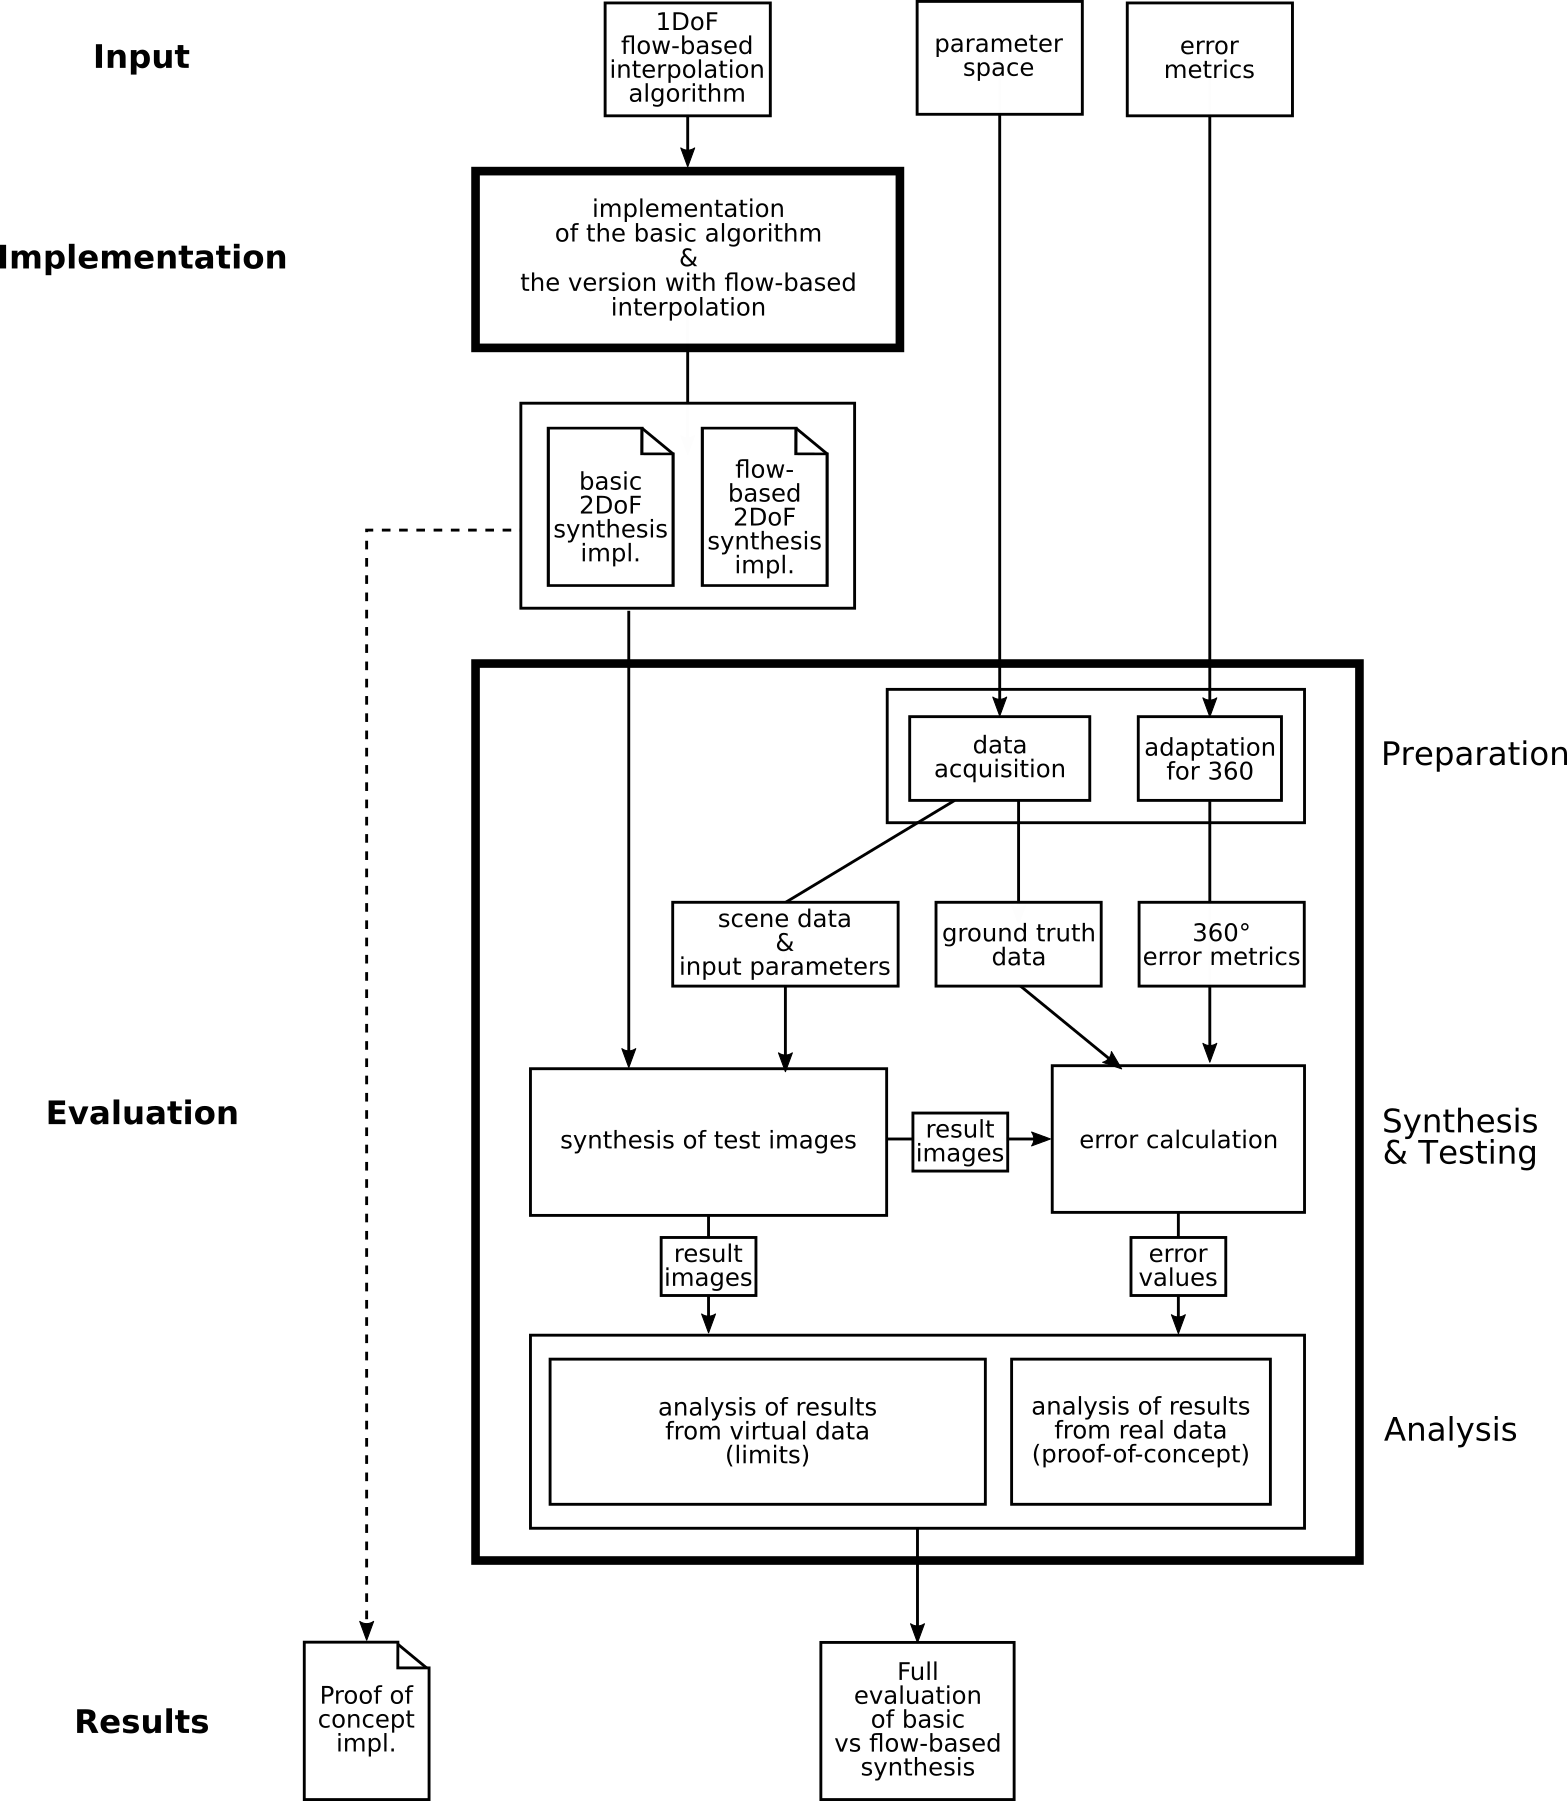
\includegraphics[width=0.9\textwidth]{01/methodology.png}
		\caption{Methodical approach}
		\label{fig:methodology}
\end{figure}


\section*{Scope}
As the number of possible different environments is infinite, as well as the positions at which images can be captured, it is necessary to limit the parameter space for testing and evaluation. First of all, only indoor scenes are examined. The scenes are assumed to be static, meaning the objects within the scene do not change their positions. To reduce the complexity of the implementation, as well as the number of necessary input images to be captured, only 2-DoF synthesis is considered. Specifically, all captured and synthesized viewpoints are located on a plane at approximate eye-level parallel to the ground. 

The parameters that will be examined in detail are:
\begin{description}
  \item[Difference between the scene geometry and the proxy geometry] The proxy geometry used in this thesis is a sphere of the approximate size of the scene. Scenes of different basic shapes, containing different objects, are tested in order to gauge the effect of the difference between the proxy geometry and the scene.
  \item[Density of captured viewpoints] The density of the captured viewpoints is an important aspect, as it is directly related to the effort required to capture a scene (the higher the necessary density, the more images need to be captured). In order to assess the effect of different densities on the accuracy of the results, different densities of captured viewpoints are tested.
    %For the evaluation in this thesis, the viewpoints used for synthesis (the ``captured viewpoints'') are arranged on a regular grid. The effect of different densities on the accuracy of the results is explored, specifically, grids of between 3m and 30cm distance are used.
  \item[Position of synthesized points relative to captured points] A synthesized viewpoint can theoretically be located anywhere within the boundaries of the scene, as long as it is at the defined eye-level. The relative position of the synthesized point to the captured points is likely to have an effect on the accuracy of the result and will be examined in more detail by synthesizing a dense grid of viewpoints within a scene.
    %This means that it can be very close to a captured viewpoint, or further away. Furthermore, it may make a difference whether the synthesized viewpoint is directly on a line between captured viewpoints. A dense grid of viewpoints is synthesized to test the effect of the relative positioning.
\end{description}

These parameters will not be examined exhaustively, as this is impossible, given the infinite possibilities of scene shapes and object placements, alone. Instead, for each parameter to be examined, a scenario is designed that tests this parameter in a reasonable context.

%Since the implementation is a basic proof-of-concept, a user study does not make much sense, since the results are expected to have some distinct artefacts. Instead, two mathematical error metrics are used to compare the 

%2-DoF synthesis without geometry in indoor environments
%variable
%quantified:
%  the location of synthesized points relative to the captured points
%  density of captured viewpoints
%
%not quantified
%  effect of objects within the scene
%  scene - model difference
%  the location of synthesized points within the scene (near walls, objects, etc)
%
%  evaluation:
%    mathematical error metrics to compare result to ground truth: mean absolute error and ssim
%
%basic proof of concept implementation \ar not perfect, real-time
%not an exhaustive evaluation of all possible parameters \& combinations
%not a comparison to other implementations (missing benchmark data and implementation of other methods is outside of scope)
%
%will be evaluating following scenarios:
%Effect of Viewpoint Density
%Viewpoint Density and Choice of Viewpoints to be Synthesized
%Position of Synthesized Viewpoints Relative to Captured Viewpoints
%Effect of Different Scenes


\section*{Contributions}
The contributions of this thesis are:
\begin{itemize}
  \item An algorithm for pixel-based 2-DoF synthesis algorithm with flow-based interpolation (``synthesis with flow-based blending'')
  \item A basic proof-of-concept implementation of this algorithm
  \item An evaluation of the results of this algorithm, including a comparison with the results of the algorithm with regular blending
\end{itemize}

The results show that in the majority of cases where the basic method with regular blending produces significant artefacts, the synthesis using flow-based blending does improve the the accuracy of the results. 

%The results of this thesis can be the basis of various future work. Since the implementation is a first attempt at combining the two methods, the problems and limitations discovered in the evaluation can be used to improve future versions. Alternative proxy geometries could be examined, potentially based on sparse scene geometry, which would improve the basic results and could lead to a distinct improvement of the flow-based results. Furthermore, parallelization and optimization could be used in order to achieve real-time framerates. 


\section*{Outline}
The structure of this thesis follows the order presented in the methodical approach: 
First, the underlying concepts of 360\degree images and optical flow are presented (Section~\ref{sec:fundamentals}), along with related work in the field of image-based synthesis (Section~\ref{sec:related_work}). Next, the ``interpolation step'' is presented, including the approach to the pixel-based 2-DoF synthesis algorithm with regular blending and flow-based blending (Section~\ref{sec:approach}) along with the details of the implementation (Section~\ref{sec:impl_details}).
For the ``evaluation step'', first the evaluation parameters and methodology are presented (Section~\ref{sec:params} and Section~\ref{sec:eval_methodology}), followed by the evaluation of the virtual scenes (Section~\ref{sec:limit_eval}) and the real scene (Section~\ref{sec:pof_eval}). Based on the insights gained in these evaluations, the limitations of the evaluation are discussed (Section~\ref{sec:limitations}).
Finally, possibilities for future work are presented, along the conclusion of the thesis (Section~\ref{chap:conclusion}).


    \chapter{Background and Related Work}

%\section{Terminology \ar Glossary?}
%
%\paragraph{Planar image}
%\paragraph{360\degree image} vs panorama
%\paragraph{Interpolation vs Synthesis} In the context of this thesis, the two terms are very similar. Interpolation is used as a type of synthesis where two images are weighted by a certain amount and added together \ldots ?
%\paragraph{Viewpoint, capture, camera} input viewpoint, output viewpoint
%Capture/Viewpoint is the term used here to signify the location and image data of a 360\degree photograph taken at a certain position in the scene
%capture is more for when the images are actually recorded
%viewpoint is more for during processing
%\paragraph{UV coordinates}
%image-based rendering vs pixel-based rendering

%\section{Fundamentals of 360\degree Images}
\section{Fundamentals}
Before diving in to image-based rendering techniques in general and the pixel-based synthesis presented in this thesis, it is important to understand some basic concepts and methods used. Since 360\degree images are used throughout, it is important to understand how such images are created and how the data can be visualized on a planar surface. Furthermore, the concept of optical flow is introduced, as it is utilized in the pixel-based synthesis.

\subsubsection{360\degree Images}\label{subsec:fundamentals_360}
Capturing an image with a 360\degree camera can be regarded mathematically as a series of projections. The sensors of a 360\degree camera can be simplified as a unit sphere covered in light receptors, where the number of light receptors corresponds to the resolution of the camera. This means that the complete surroundings are projected onto this sphere by way of incoming light rays (see Figure~\ref{fig:lightrays}). The limited number of sensors acts as a discretizer and captures a specific color value for each resolution point (pixel). At this point, the data is in \emph{world coordinates}, meaning that each pixel value corresponds to a point on the surface of the unit sphere. 
\missingfigure{incoming light rays on unit sphere, maybe with uv indices \label{fig:lightrays}}

As the majority of viewing devices is planar (e.g. computer or smartphone screens), the image data needs to be projected to a flat surface in order to be viewed on a flat screen. This problem is well-known in cartography, and several different types of projections exist, which transform the data from world coordinates to \emph{image coordinates}. No data loss \ar conversions between projections possible.

\subsubsection{Projections for Planar Viewing \label{subsec:projections} \cite{hdrbook}}
The most common projections for 360\degree images are the \emph{cube map}, the \emph{ideal mirrored sphere}, the \emph{angular map},  and the \emph{equirectangular} representaion, also known as \emph{latitude-longitude} (\emph{latlong}) \cite{hdrbook}.

\paragraph{Cube Map}
The cube map is a mapping that splits the data into six separate square views, one in each direction (top, front, left, right, back, bottom). This is the equivalent of capturing the surroundings with six different cameras with a field of view of 90\degree each, and then stitching the resulting images into a shape that can be ``folded'' into a cube (see Figure~\ref{fig:cubemap-intro}), which also gives this mapping its name.

Due to the projection of a spherical surface to a plane, there is some distortion towards the edges of each face. However, this distortion is comparable to the distortion at the edges of a regular, planar image, which is a significant advantage compared to other mappings. The disadvantage is that each face is projected separately, which leads to directional discontinuities at the many seams. This type of mapping is often used to simulate complex environments in 3D scenes (e.g. for game or animation graphics), as it is easy to use and reduces render time significantly compared to a 3D model of the same environment.
\cite{hdrbook}

\paragraph{Ideal Mirrored Sphere}
The ideal mirrored sphere is a mapping to a circle within a square. It represents how the surroundings would be reflected by a perfect mirrored sphere, given the size of the sphere was considerably smaller than the distance to the surroundings. This mapping, like all the mappings presented here, shows the complete surroundings, albeit very distorted toward the edges. Figure~\ref{fig:sphere-intro}b shows where each direction is mapped and the extent of the distortion. It is clear that the farther away from the ``front'' area, the more distorted the mirrored sphere mapping is. The ideal mirrored sphere mapping can be used for calculating average illumination color for high dynamic range calculations, however, the type of distortion at the edges can cause problems with sampling, which is why the angular map mapping tends to be preferred.
\cite{hdrbook}

\paragraph{Angular Map}
At first sight, the angular map seems very similar to the ideal mirrored sphere. It also maps to a circle within a square, however it samples the input in such a way that the back of the image is allotted more space and is less distorted than the mirrored sphere (see Figure~\ref{fig:angular-intro}). This mapping is also used for high dynamic range calculations.

\paragraph{Equirectangular}
The equirectangular, or latitude-longitude mapping is a common type of mapping in cartography. The data is mapped to a rectangular image space, in which the width is twice the height. The azimuth (around the circumference) of the world coordinates is mapped to the map's horizontal coordinate and the elevation to the vertical coordinate. The main problem of this representation is well known in cartography: The distortion increases significantly towards the poles, as can be seen in Figure~\ref{fig:latlong-intro}. Otherwise, this mapping is convenient as it has very few seams. It is used as a storage format for 360\degree images.

\paragraph*{}
All of these projections are static, showing the entirety of the 360\degree image at once. It is also possible to view 360\degree images interactively. In this case the field of view tends to be limited, so only a certain part of the image needs to be projected: the part of the image the viewer is ``facing'' virtually. Once the viewing direction has been determined, the projection can be calculated such that the center of the image has minimal distortion. Theoretically, any of the above projections could be used for this. 

\begin{figure}
\centering
    \begin{subfigure}[t]{0.5\textwidth}            
            \centering
            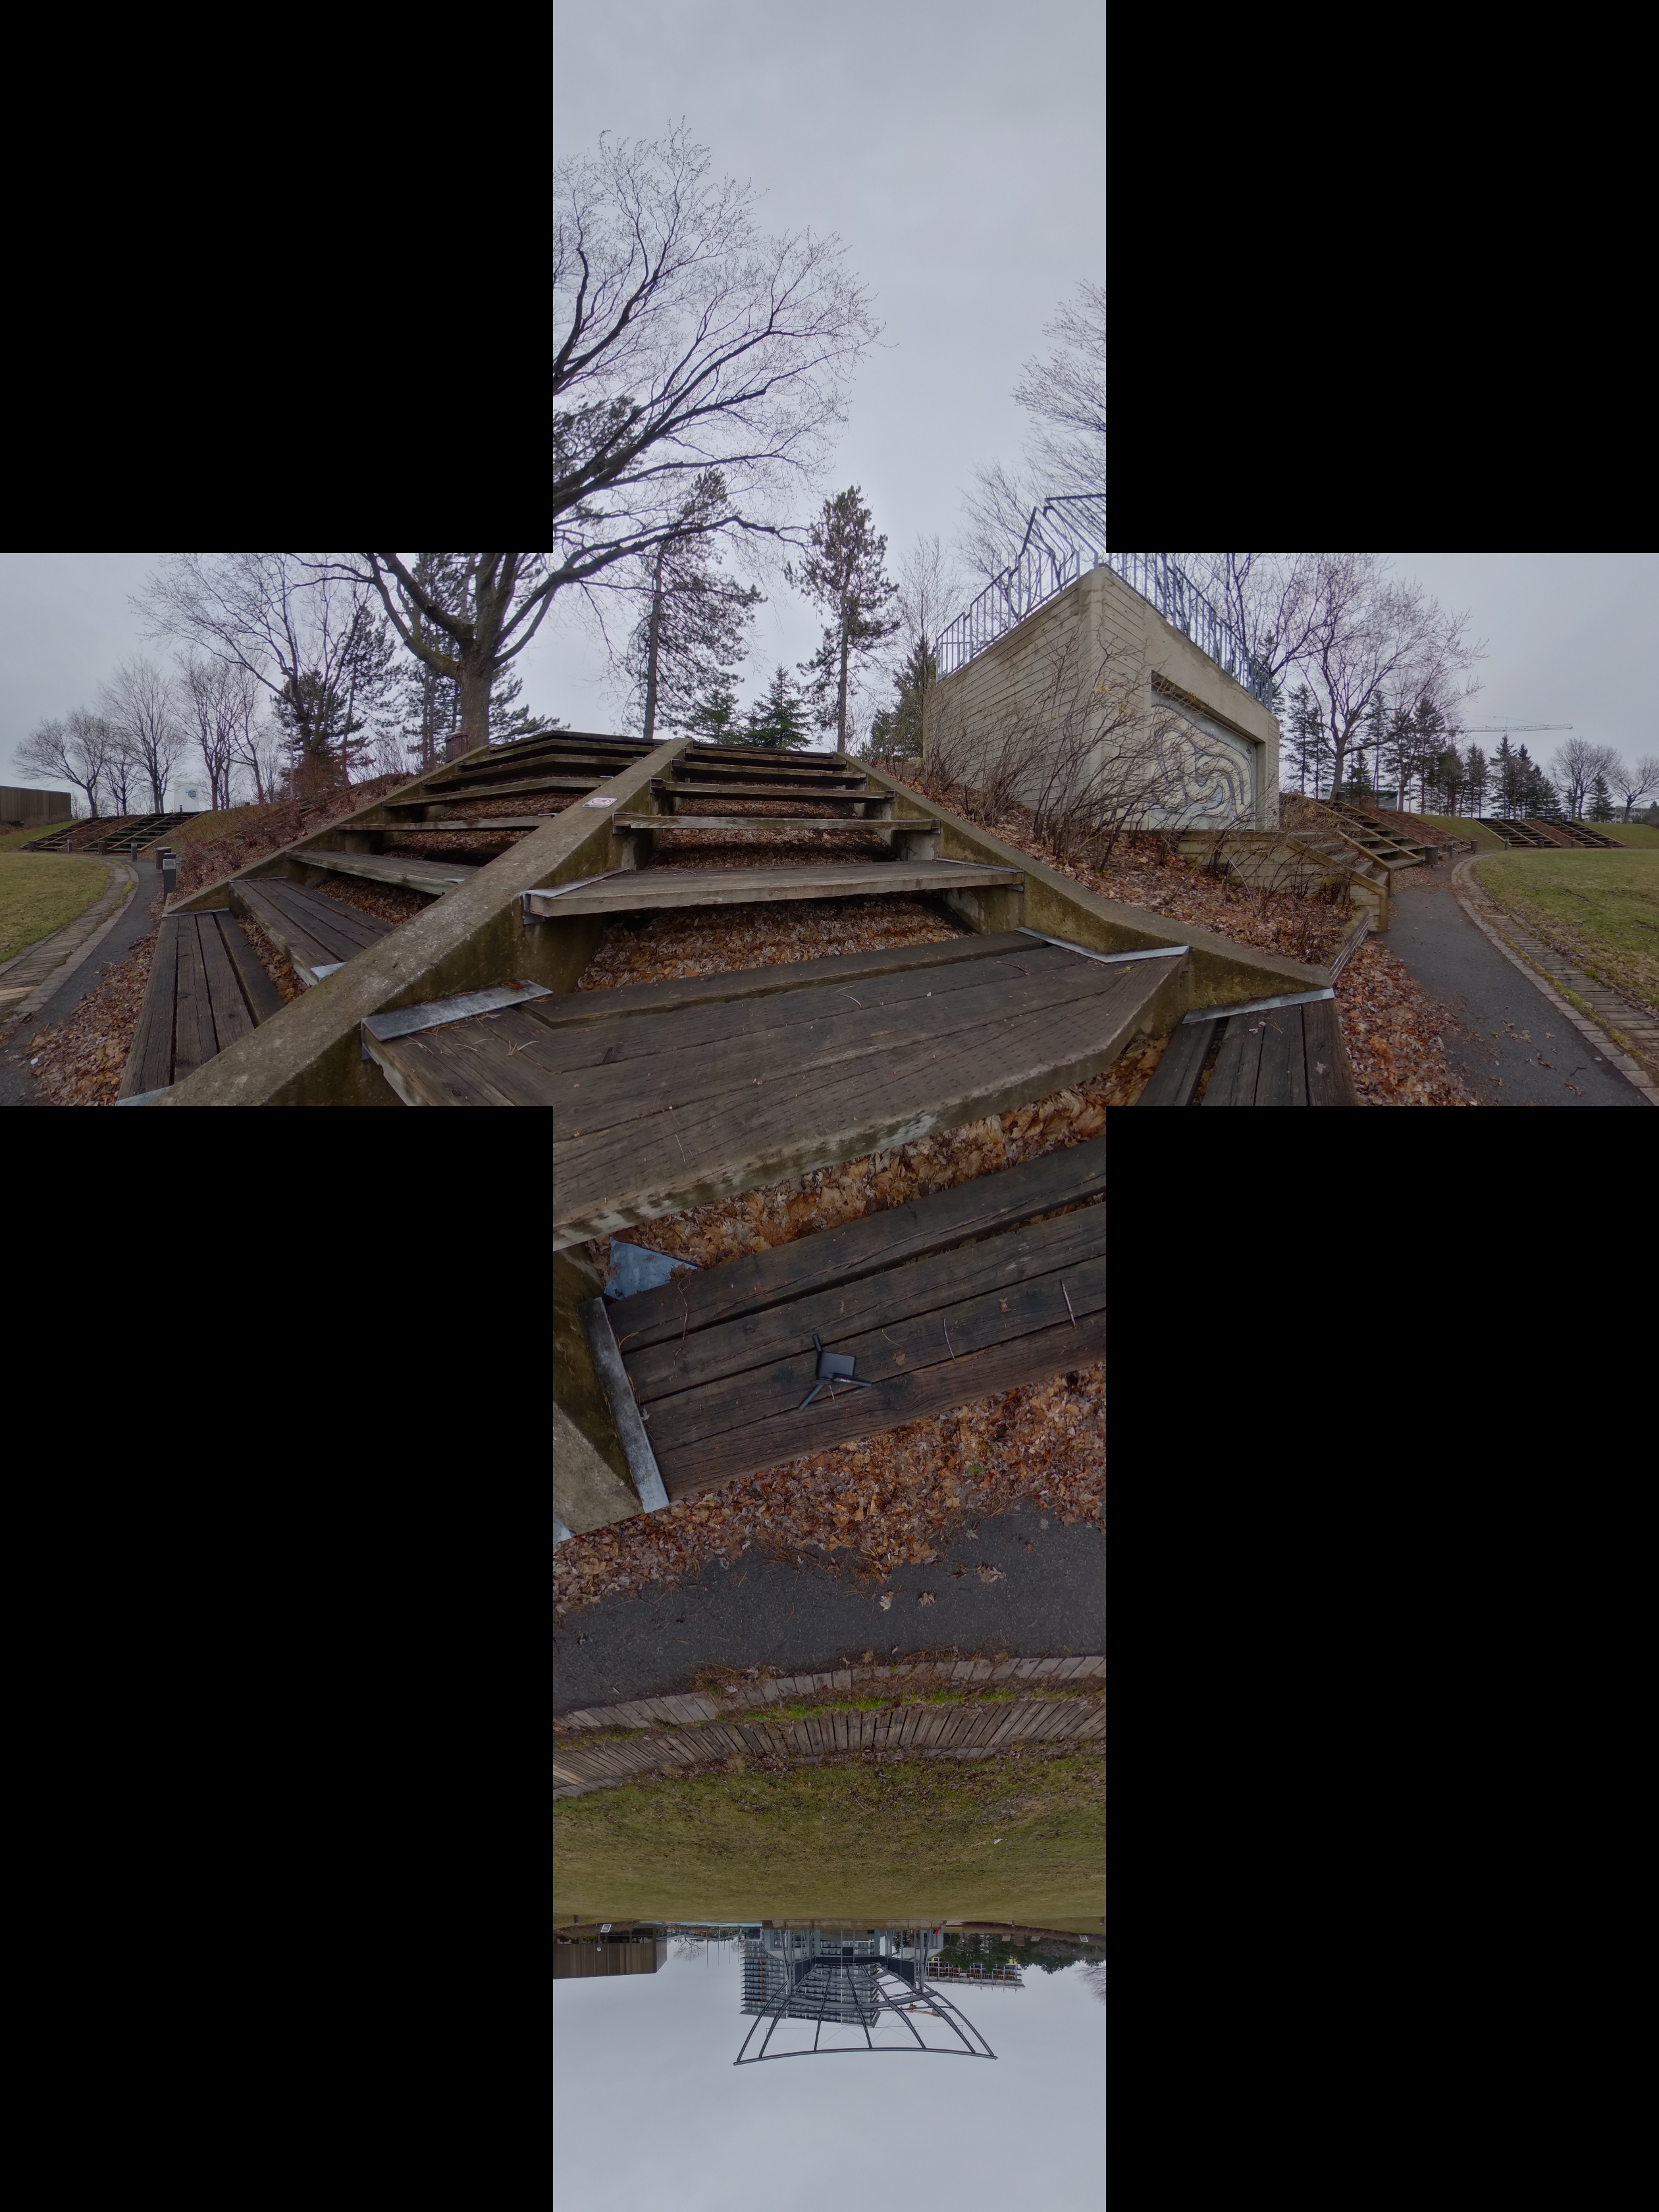
\includegraphics[width=0.5\textwidth]{02/mapping_cube_photo.jpg}
            \caption{360\degree image as a cube map}
    \end{subfigure}%
     %add desired spacing between images, e. g. ~, \quad, \qquad etc.
      %(or a blank line to force the subfigure onto a new line)
    \begin{subfigure}[t]{0.5\textwidth}
            \centering
            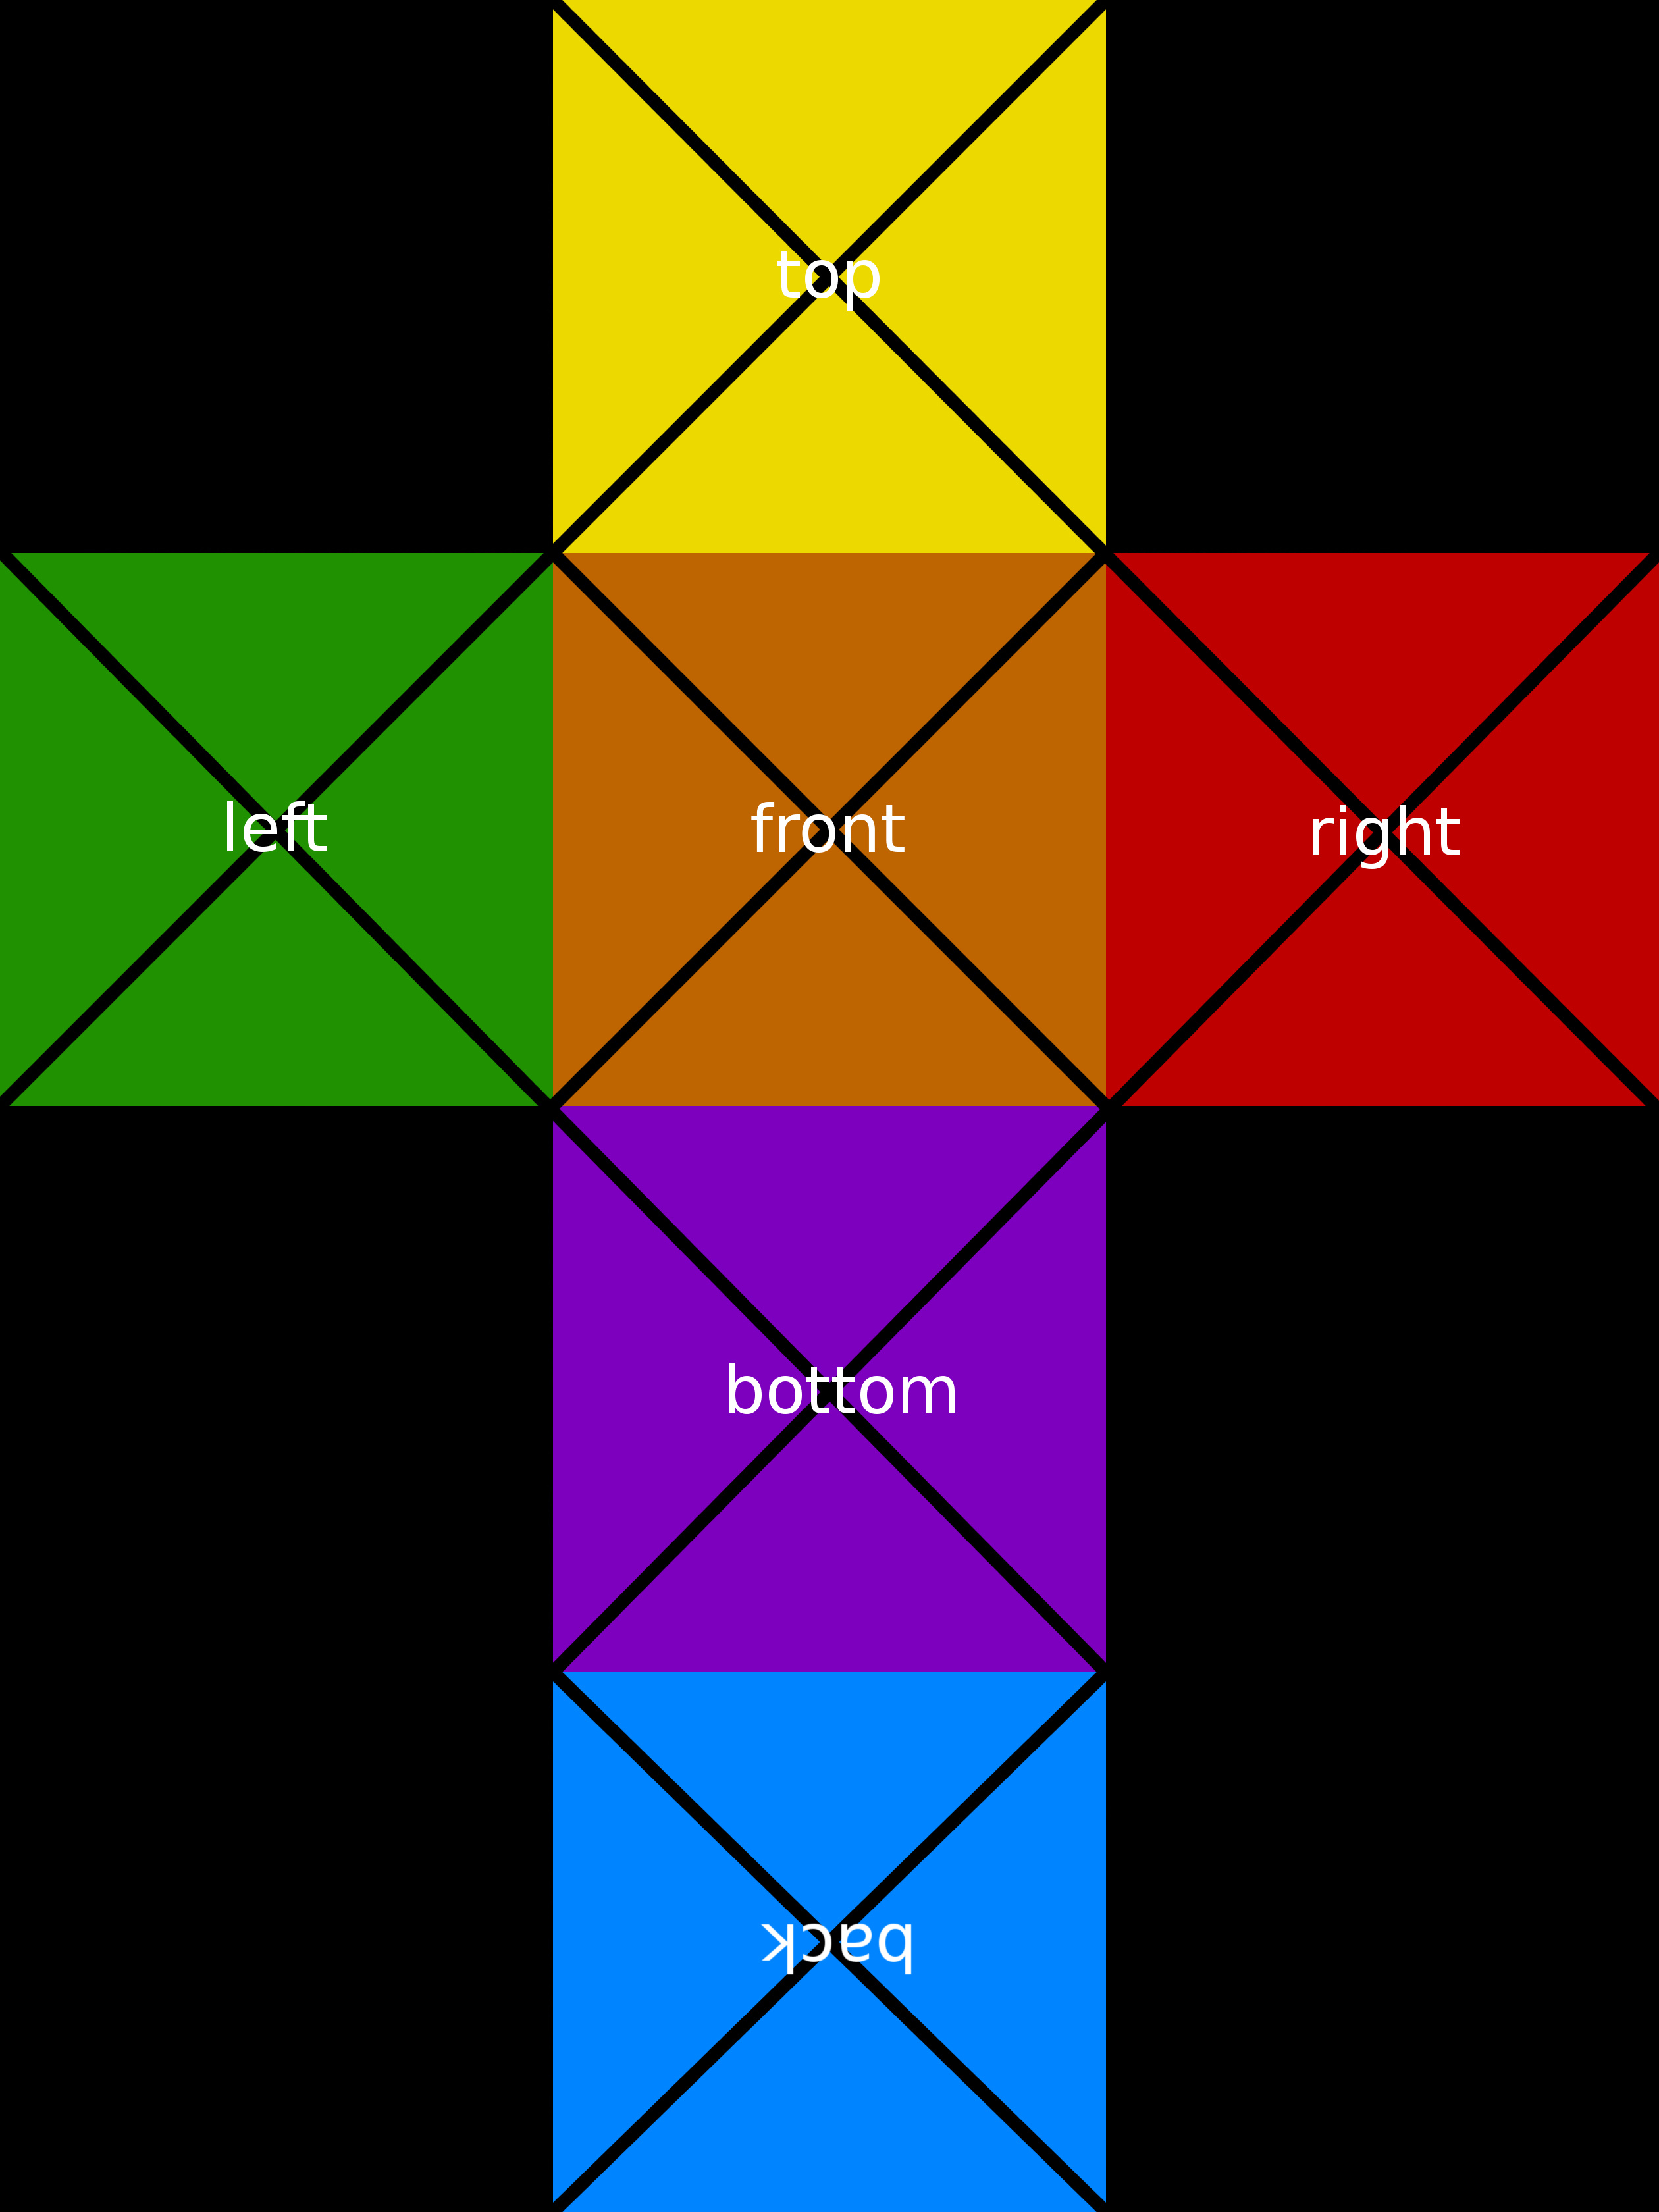
\includegraphics[width=0.5\textwidth]{02/mapping_cube.jpg}
            \caption{Visualization for comparison to other mappings \protect\footnotemark}
    \end{subfigure}
    \caption[Cube map mapping]{The cube map mapping}\label{fig:cubemap-intro}

    \quad
    \begin{subfigure}[t]{0.5\textwidth}
            \centering
            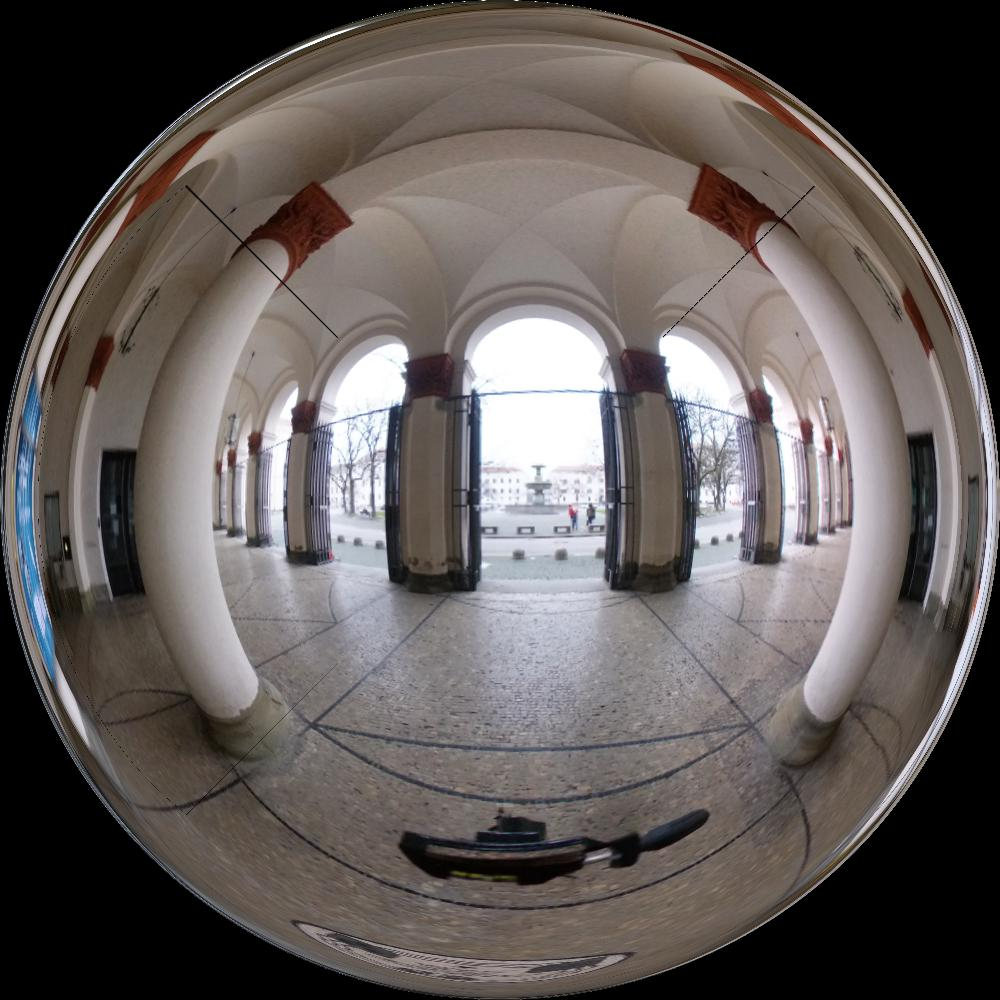
\includegraphics[width=0.5\textwidth]{02/mapping_sphere_photo.jpg}
            \caption{360\degree image as a mirrored sphere mapping}
    \end{subfigure}%
     %add desired spacing between images, e. g. ~, \quad, \qquad etc.
      %(or a blank line to force the subfigure onto a new line)
    \begin{subfigure}[t]{0.5\textwidth}
            \centering
            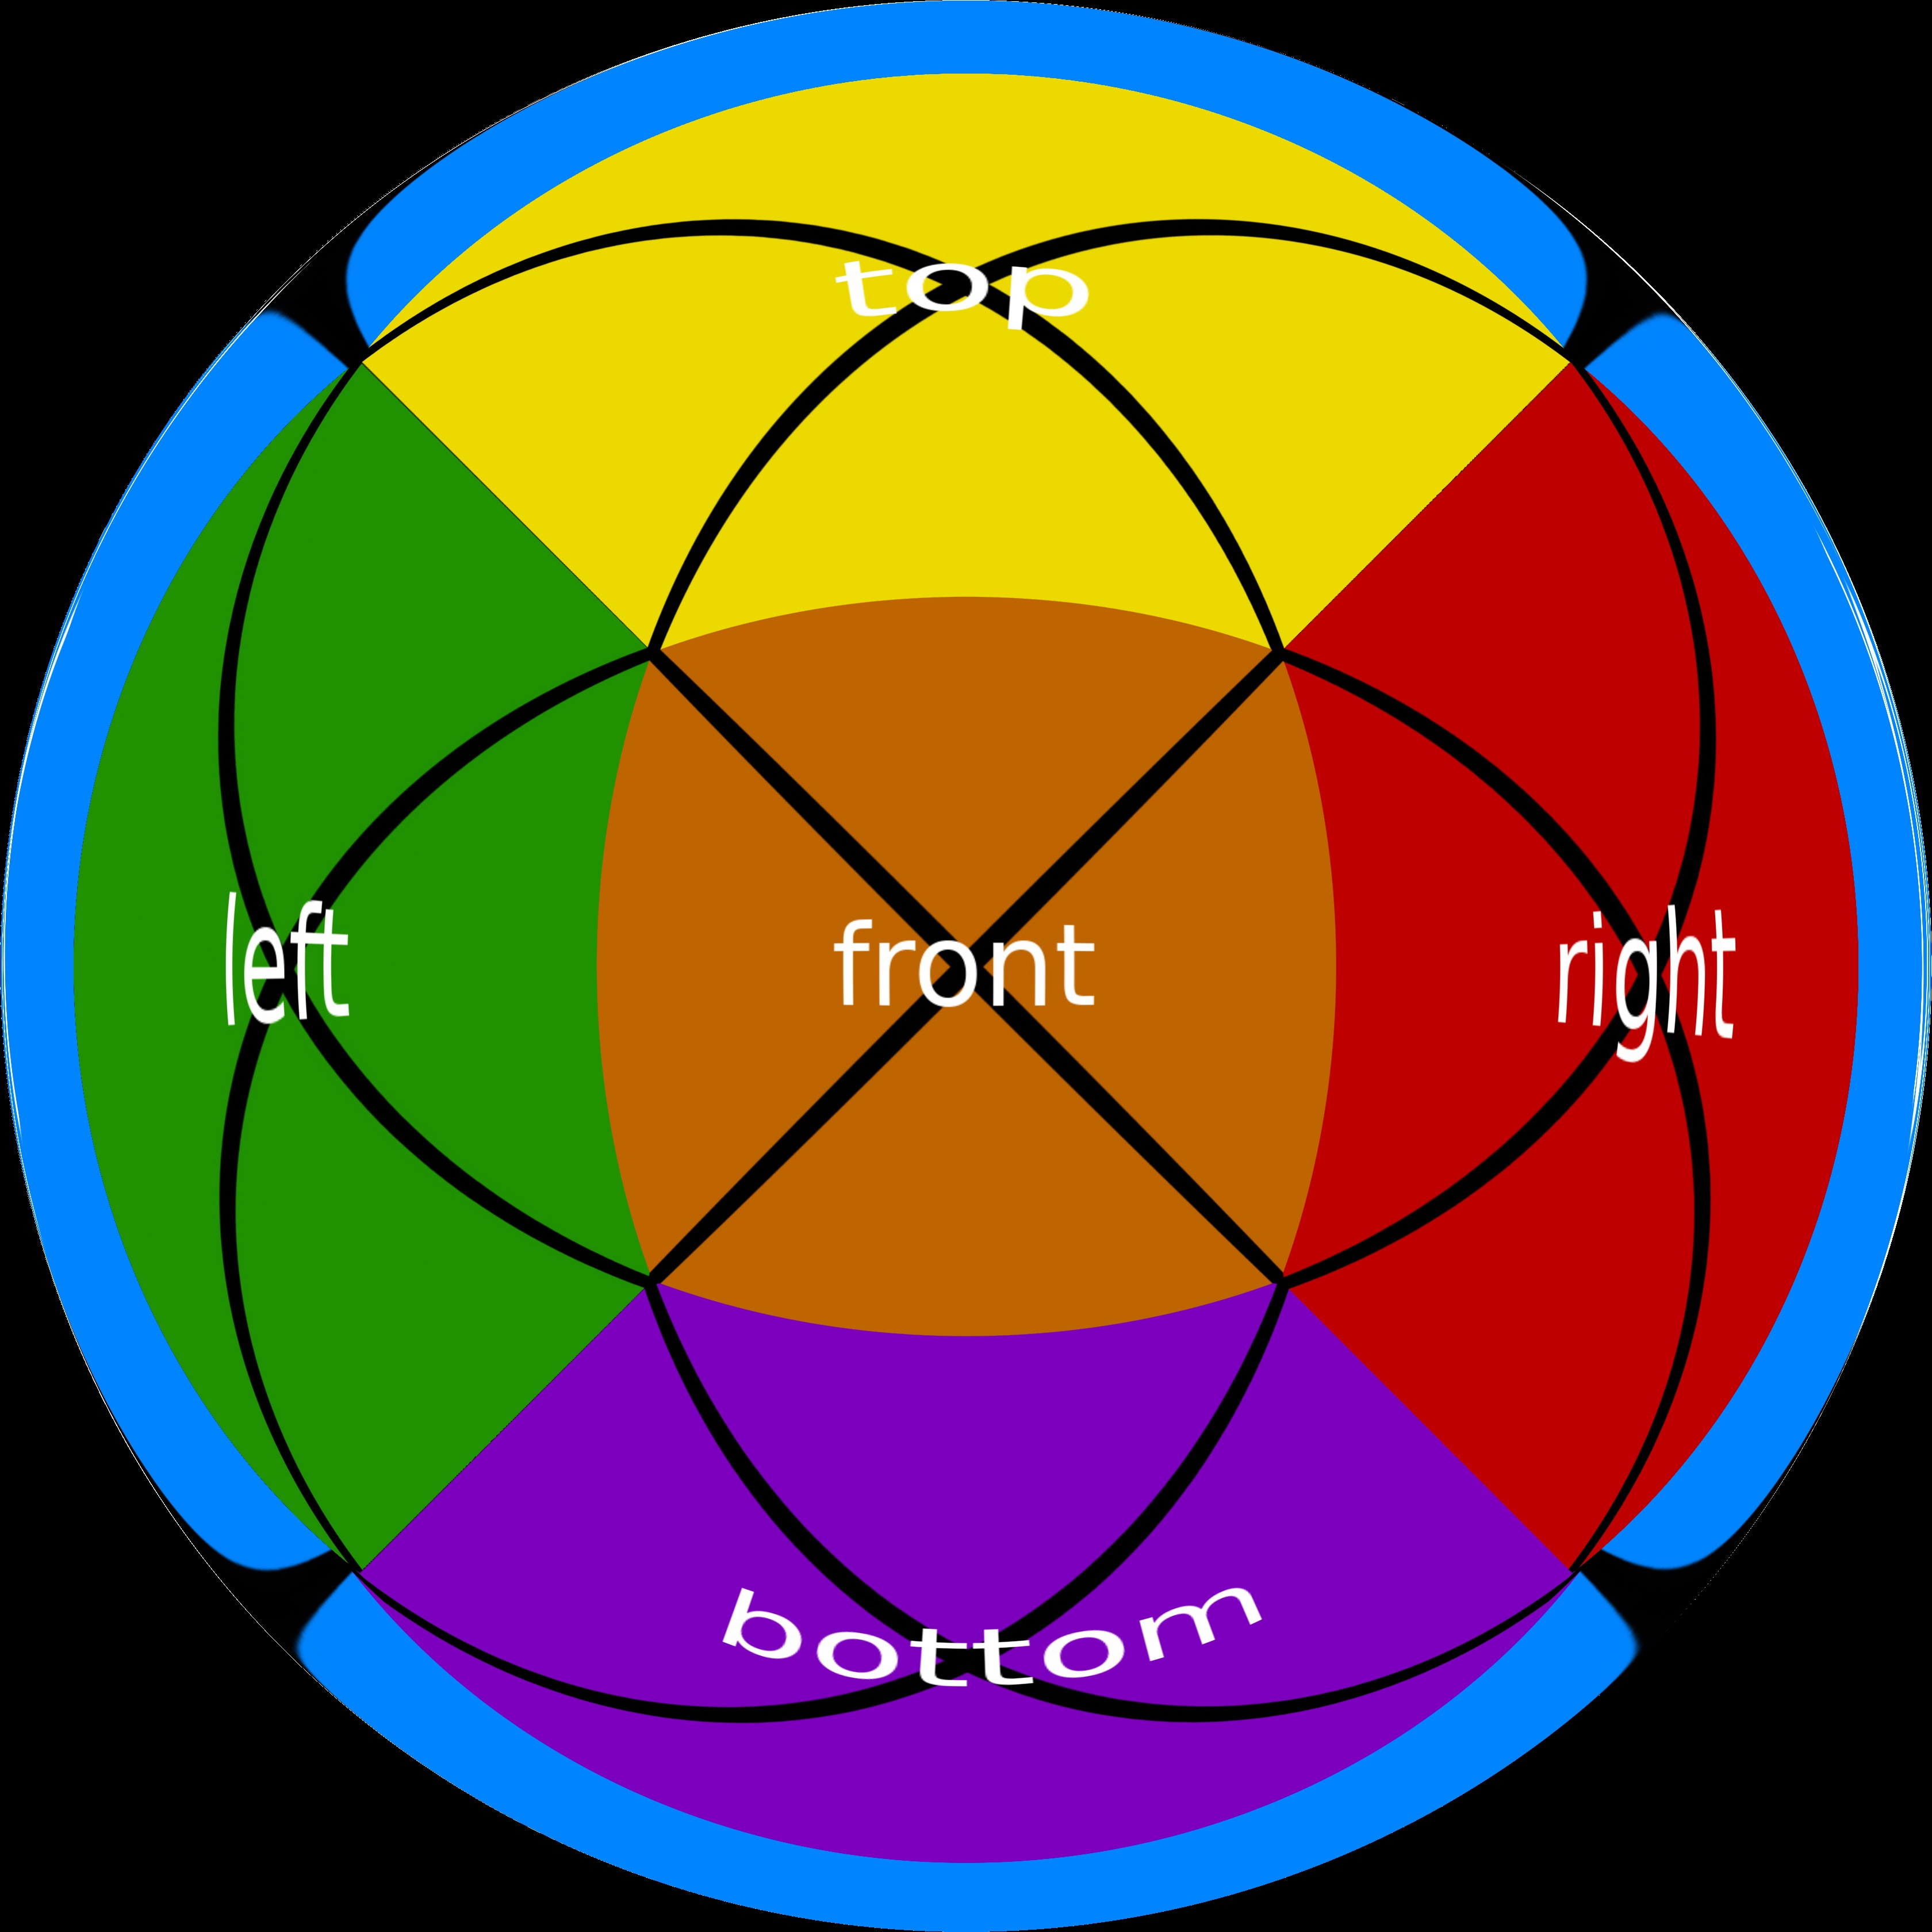
\includegraphics[width=0.5\textwidth]{02/mapping_sphere.jpg}
            \caption{Visualization for comparison to other mappings}
    \end{subfigure}
    \caption[Mirrored sphere mapping]{The mirrored sphere mapping}\label{fig:sphere-intro}

    \quad
    \begin{subfigure}[t]{0.5\textwidth}            
            \centering
            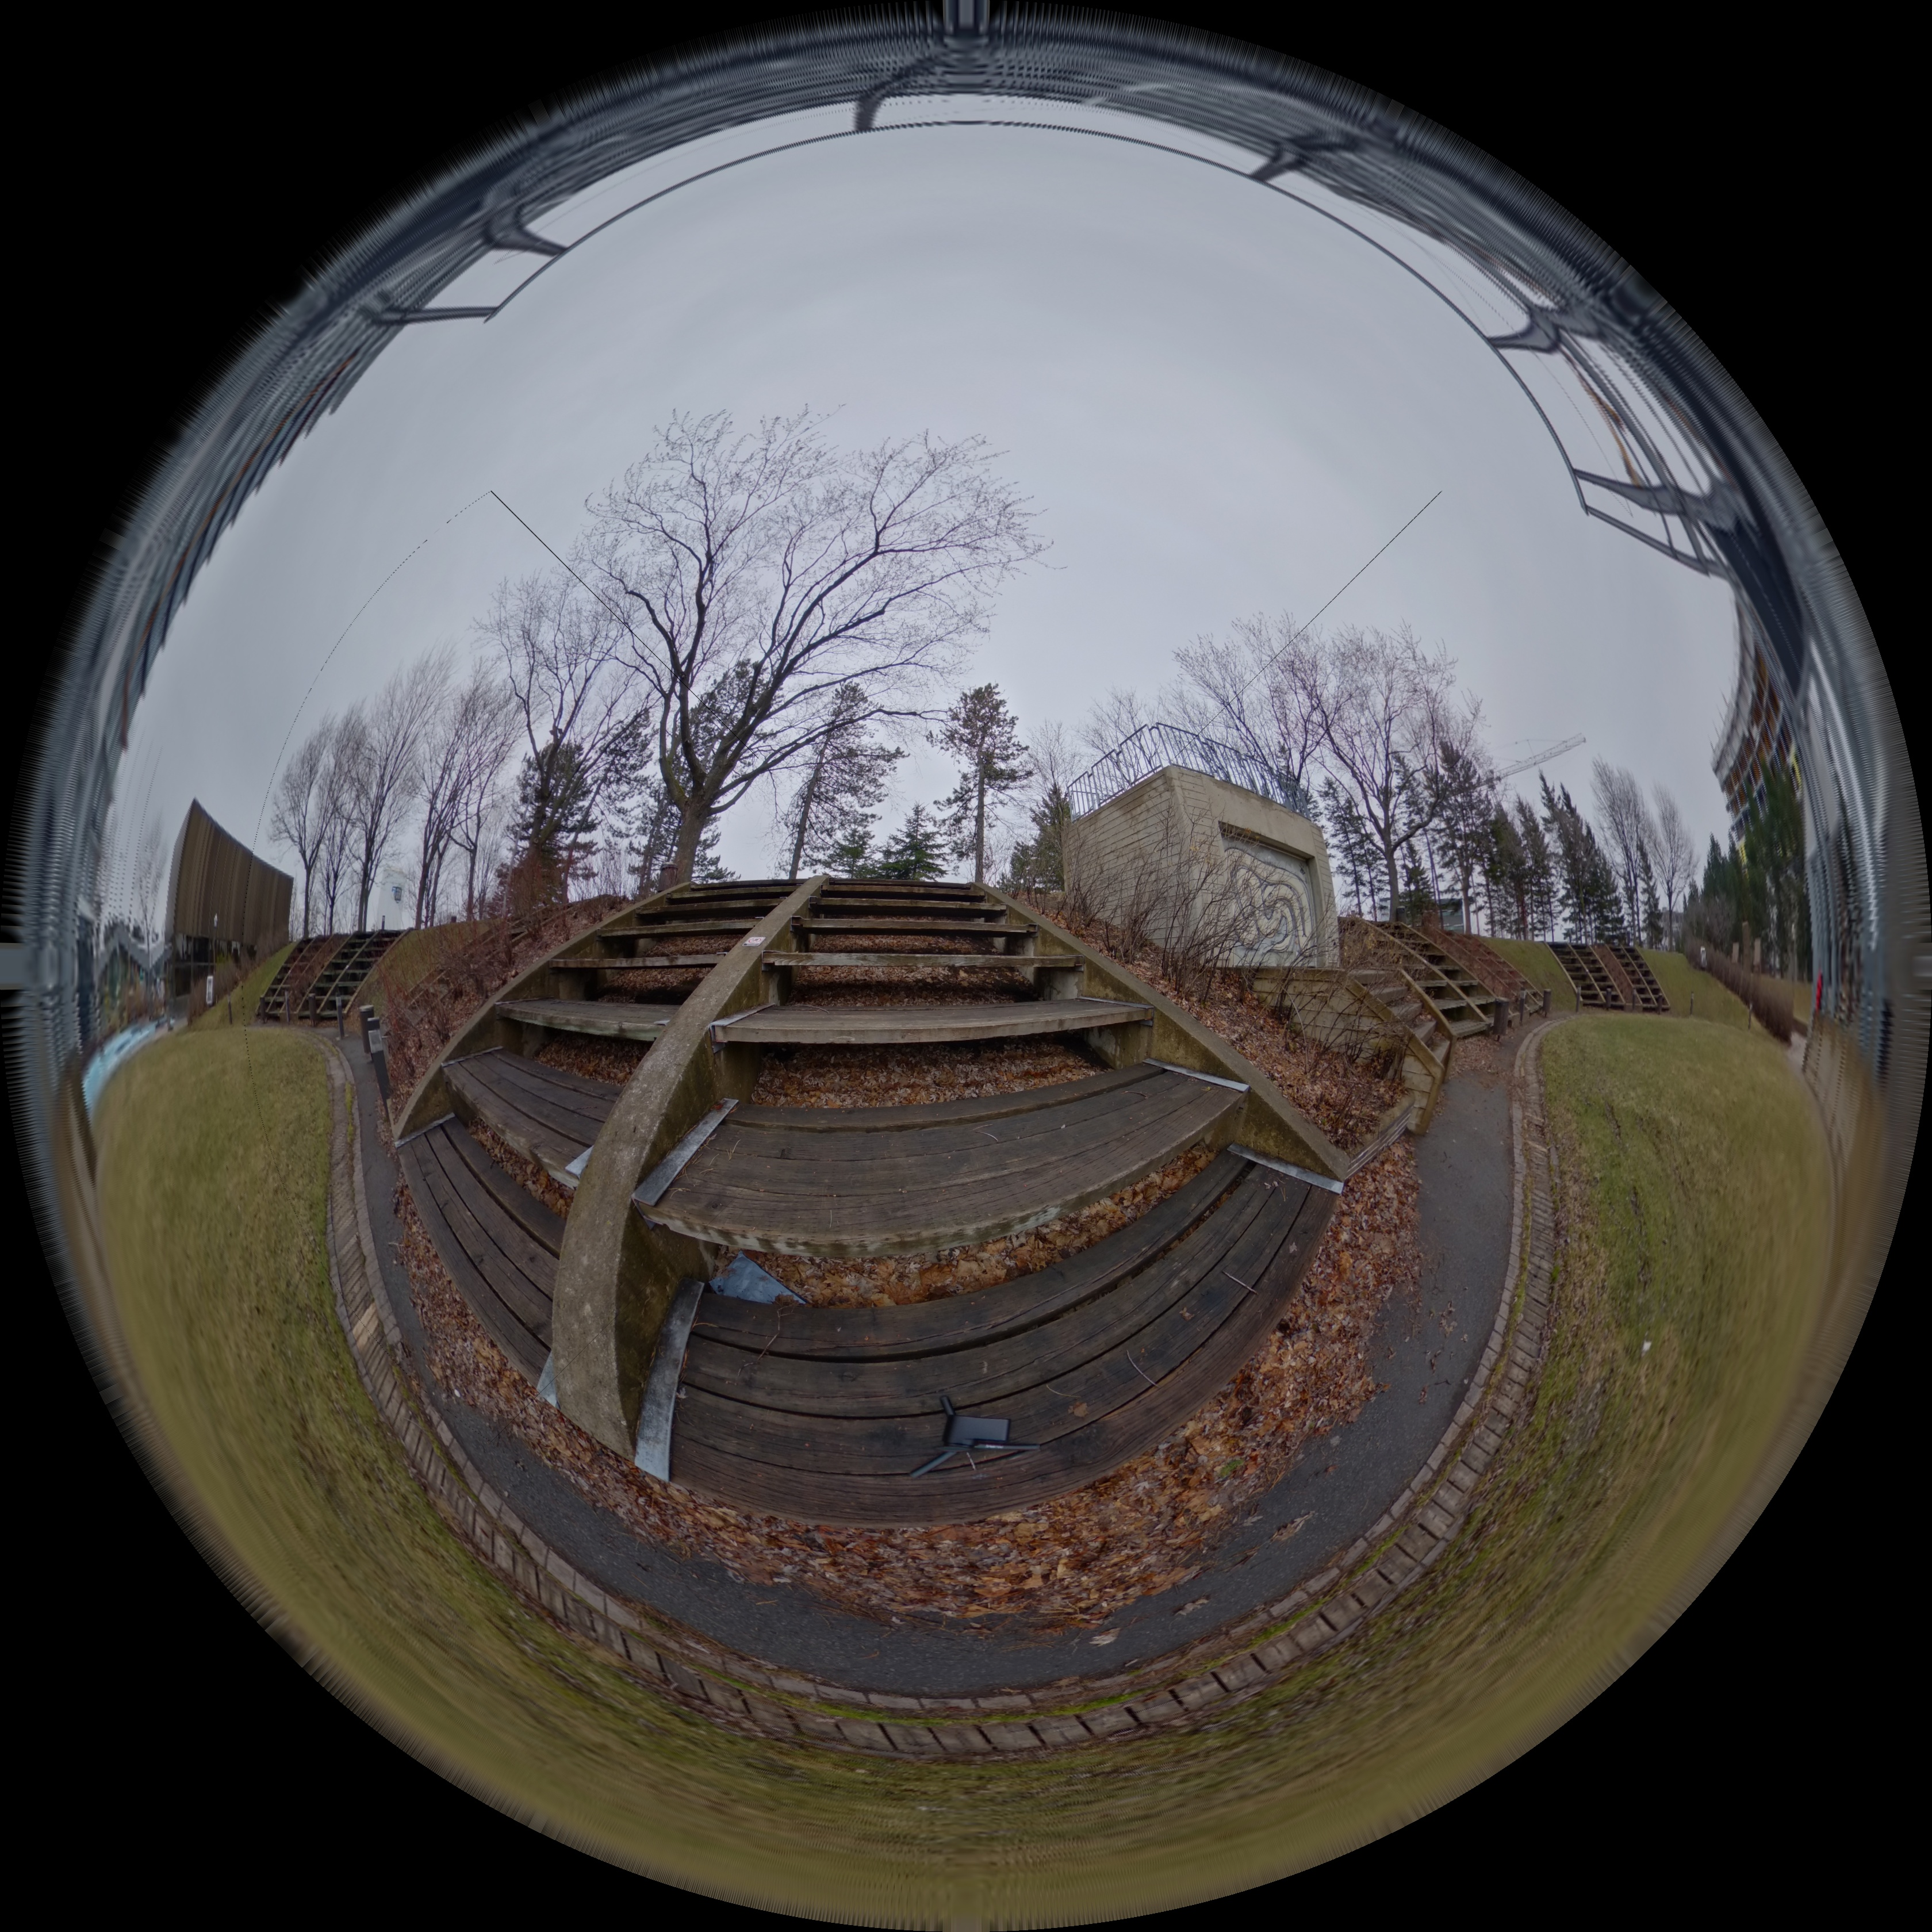
\includegraphics[width=0.5\textwidth]{02/mapping_angular_photo.jpg}
            \caption{360\degree image as an angular mapping}
    \end{subfigure}%
     %add desired spacing between images, e. g. ~, \quad, \qquad etc.
      %(or a blank line to force the subfigure onto a new line)
    \begin{subfigure}[t]{0.5\textwidth}
            \centering
            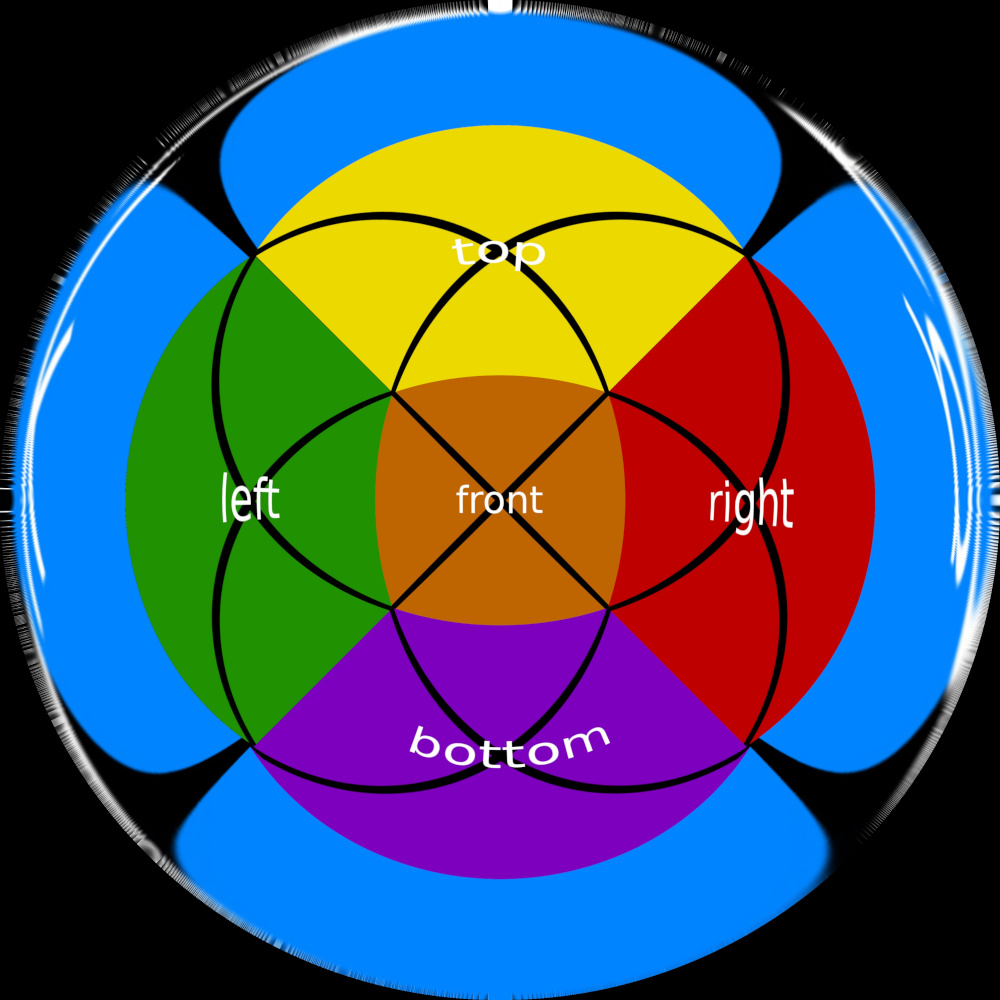
\includegraphics[width=0.5\textwidth]{02/mapping_angular.jpg}
            \caption{Visualization for comparison to other mappings}
    \end{subfigure}
    \caption[Angular mapping]{The angular mapping}\label{fig:angular-intro}

    \quad
    \begin{subfigure}[t]{0.5\textwidth} 
            \centering
            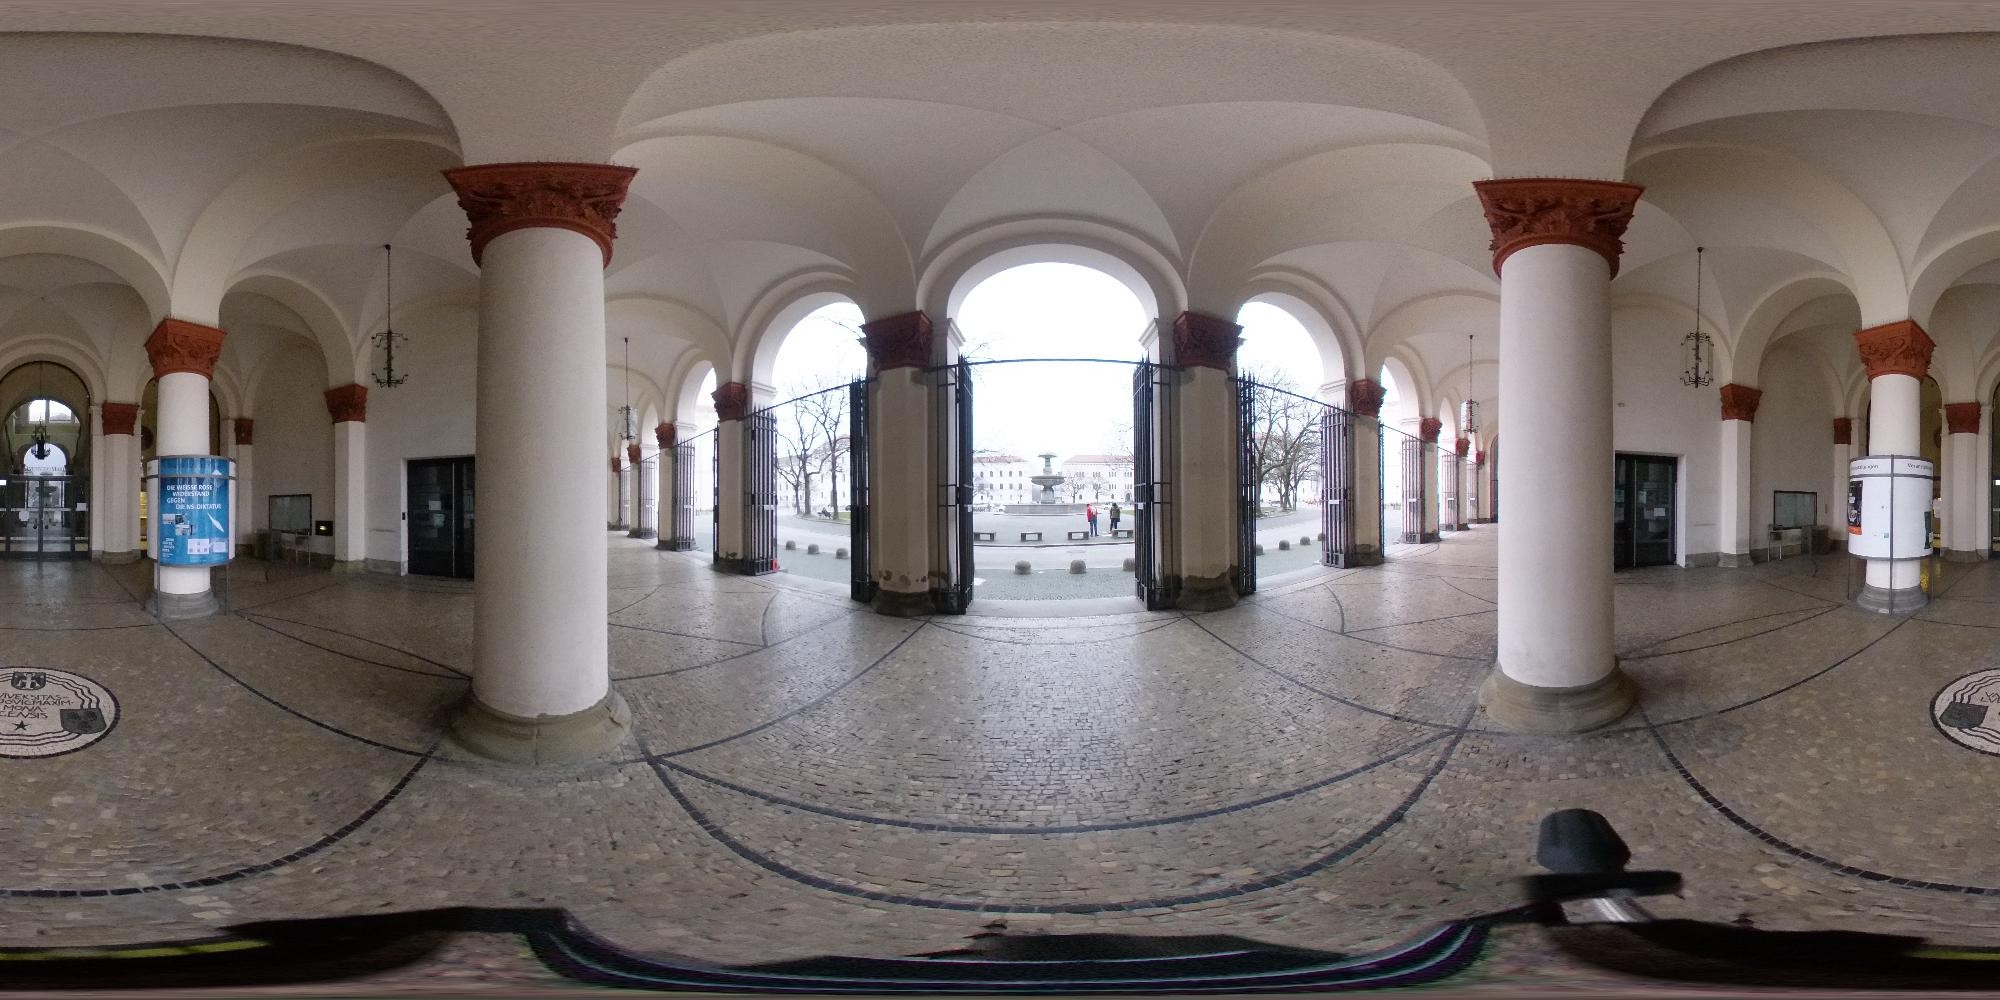
\includegraphics[width=0.9\textwidth]{02/mapping_latlong_photo.jpg}
            \caption{360\degree image as a latlong mapping}
    \end{subfigure}%
     %add desired spacing between images, e. g. ~, \quad, \qquad etc.
      %(or a blank line to force the subfigure onto a new line)
    \begin{subfigure}[t]{0.5\textwidth}
            \centering
            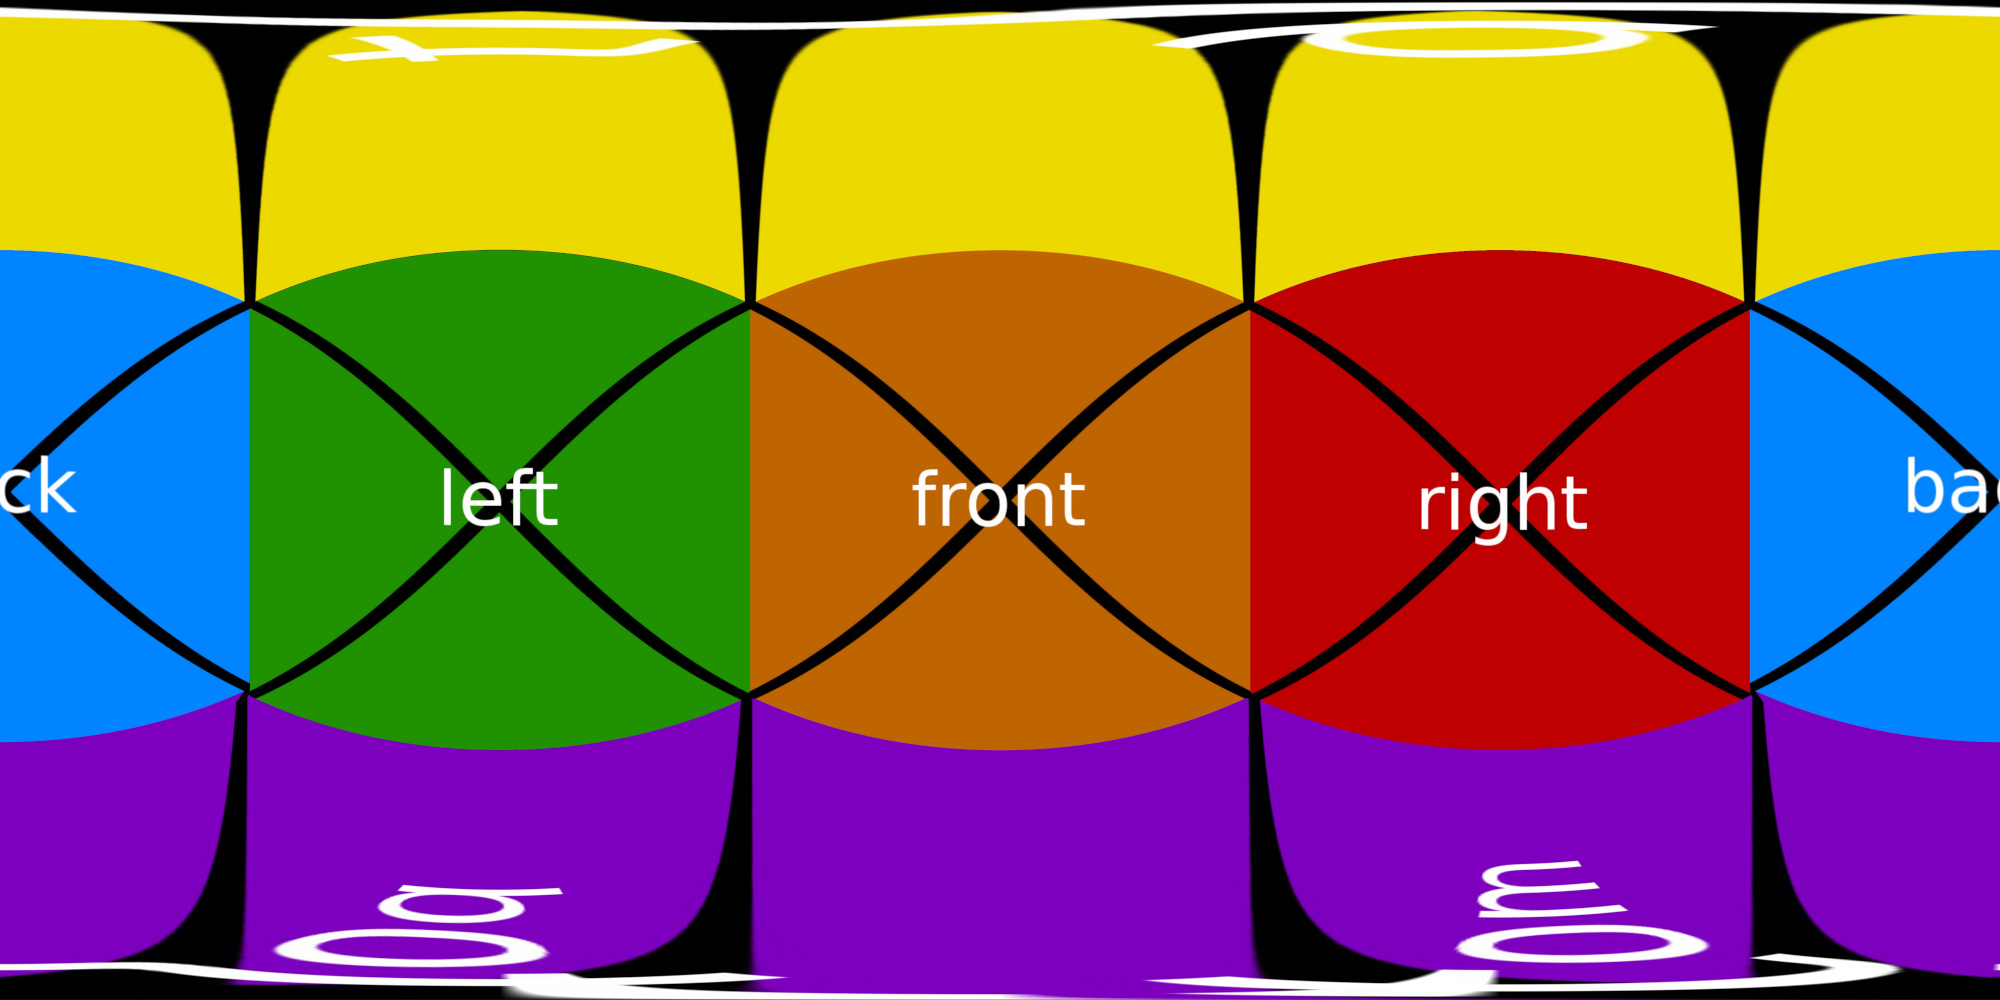
\includegraphics[width=0.9\textwidth]{02/mapping_latlong.jpg}
            \caption{Visualization for comparison to other mappings}
    \end{subfigure}
    \caption[Latlong mapping]{The latlong mapping}\label{fig:latlong-intro}
  \end{figure}
  \footnotetext{Figure~\ref{fig:cubemap-intro}b does not correctly represent the distortion in cube maps. It was chosen as a baseline because cube maps have relatively small distortion compared to other mappings and it visualizes clearly which parts of the image are mapped where.}


\subsubsection{Optical Flow}
Optical flow describes the displacement of specific points between two images. It is generally used on consecutive frames of video sequences, for example for semantic segmentation, structure-from-motion, data compression or other applications where information about movement between images is required. To illustrate, Figure~\ref{fig:of_example_bike} shows two consecutive frames of a video sequence. On a high level, an optical flow algorithm should recognize that the pixels representing the bicyclist are moving towards the bottom left of the image, and the pixels representing the background are moving to the right (because the camera is panning slightly to the left).

\todo{investigate why there is vertical space between the paragraphs}
There are two types of optical flow: Sparse optical flow and dense optical flow. Sparse optical flow algorithms calculate the motion of several select points that can be either chosen manually, or by some kind of automatic selection (e.g. based on features). This type of optical flow can be used to track only specific objects in a scene (e.g. the direction and relative velocity of a certain car in traffic).

Dense optical flow algorithms compute the motion of \emph{each pixel} between two images, which yields a more exact result than sparse optical flow. This can be used for more general object tracking (e.g. direction and relative velocity of complete surroundings in traffic), to estimate 3D geometry (in structure-from-motion algorithms), or to identify static sections of the image for video compression. Dense optical flow can also be used for image synthesis, such as in Richardt et. al's Megastereo \cite{megastereo} described in section~\ref{subsec:megastereo}, which is also the basis of the flow-based interpolation presented in this thesis.

There are a number of optical flow algorithms, ranging from methods using parametrization, or regularization \cite{of-survey}, to methods relying on Deep Learning \cite{of-deep}. Although these algorithms differ greatly in approach, they have in common the type of result, which is a vector field. For dense optical flow, this vector field contains a vector for each pixel, describing the displacement of this pixel between the input images. Sparse optical flow only contains a vector for each pre-chosen point, not for every pixel.

Figure~\ref{fig:of_vis} shows two different visualizations of the vector field calculated by the dense optical flow algorithm by Farneb\"ack \cite{farneback} between the frames in Figure~\ref{fig:of_example_bike}. Visualization \emph{a} is a color-based visualization: the hue encodes the vector direction, the saturation encodes the vector length for each pixel. Using this visualization, it is possible to roughly distinguish two separately moving areas of the image, which could be used for semantic segmentation. Visualization \emph{b} shows the pixel displacements with vectors: the origin of the vector is shown by a point and the direction and length of the vector are represented by a line.

These visualizations can help in understanding if and how well an optical flow algorithm is working. Although there are a large number of different algorithms, most of them still struggle with common issues such as occlusions, too-large displacements and intensity changes \cite{of-survey}. Occlusions are problematic, since the displacements between two images may reveal or cover image areas that, as a result, have no correspondence in the previous image. This problem is exacerbated when displacements are very large (e.g. due to fast-moving objects). Large displacements are also problematic by and of themselves, as most algorithms are not designed to handle them. How these limitations affect the use of optical flow for image synthesis will be explored in Section~\ref{evaluation-1D}.

\begin{figure}
\centering
    \begin{subfigure}[t]{0.5\textwidth}            
            \centering
            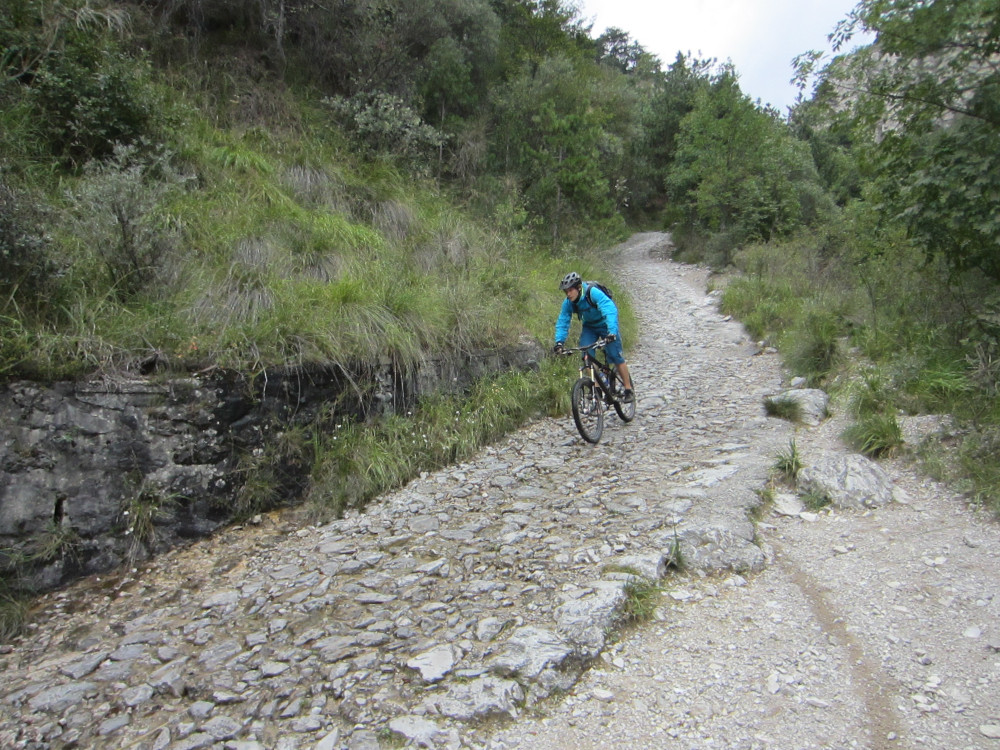
\includegraphics[width=0.9\textwidth]{02/of_example1.jpg}
            \caption{Frame 1}
    \end{subfigure}%
     %add desired spacing between images, e. g. ~, \quad, \qquad etc.
      %(or a blank line to force the subfigure onto a new line)
    \begin{subfigure}[t]{0.5\textwidth}
            \centering
            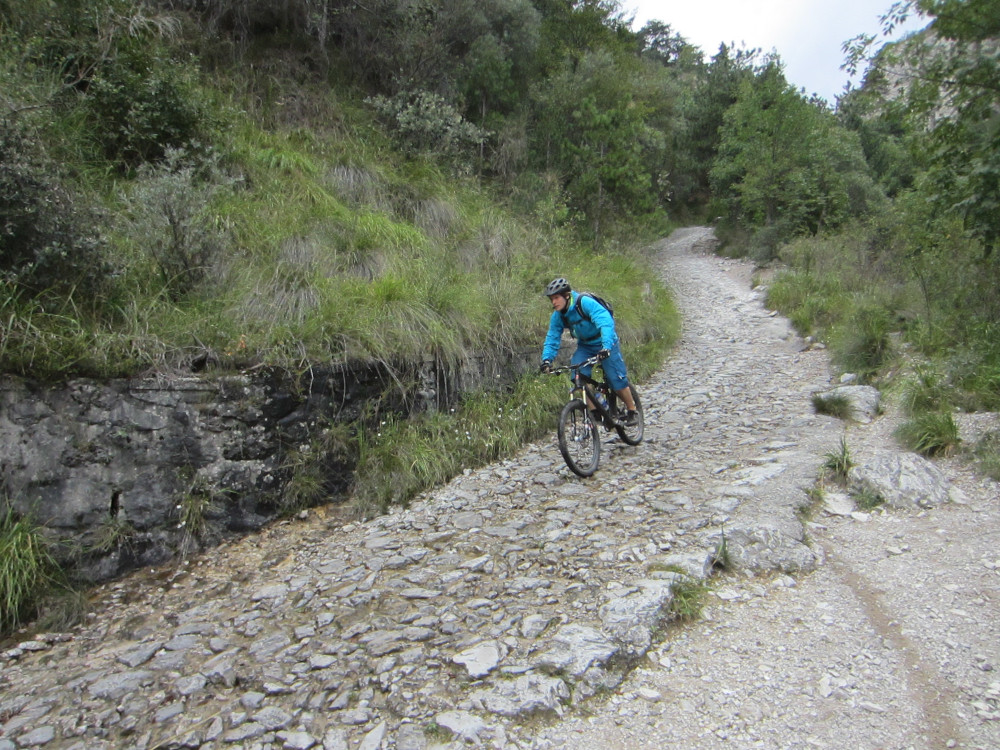
\includegraphics[width=0.9\textwidth]{02/of_example2.jpg}
            \caption{Frame 2}
    \end{subfigure}
    \caption[Optical flow example]{Example frames that optical flow is calculated on}\label{fig:of_example_bike}

    \quad
    \begin{subfigure}[t]{0.5\textwidth}            
            \centering
            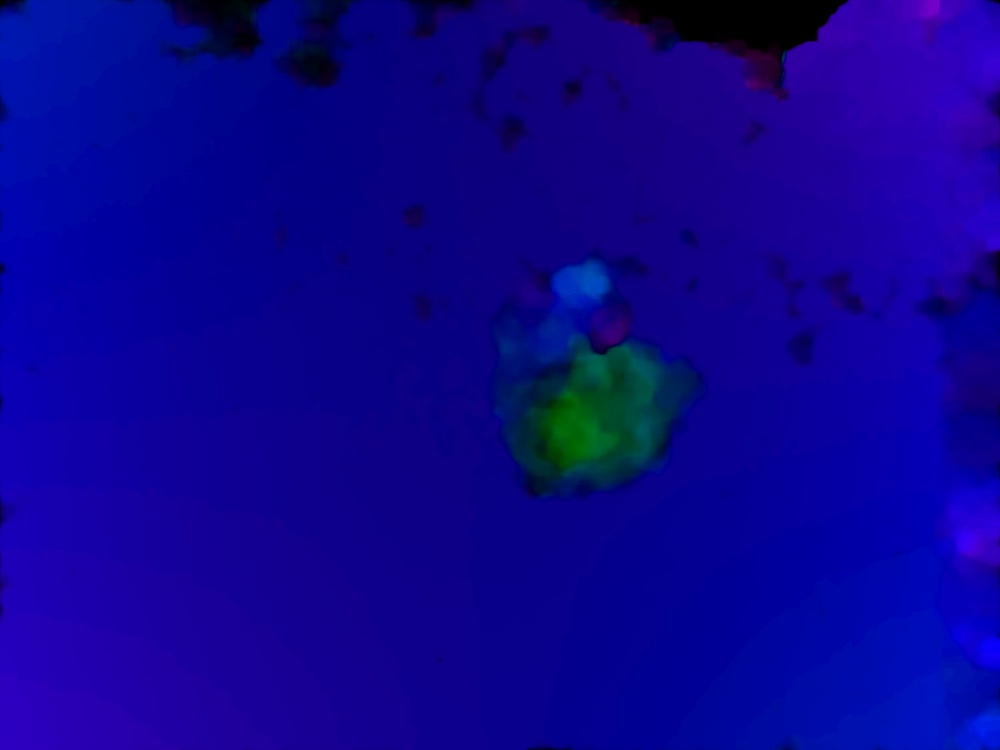
\includegraphics[width=0.9\textwidth]{02/of_vis1.jpg}
            \caption{Visualization of optical flow with color: the hue encodes the vector direction, the saturation encodes the vector length for each pixel.}
    \end{subfigure}%
     %add desired spacing between images, e. g. ~, \quad, \qquad etc.
      %(or a blank line to force the subfigure onto a new line)
    \begin{subfigure}[t]{0.5\textwidth}
            \centering
            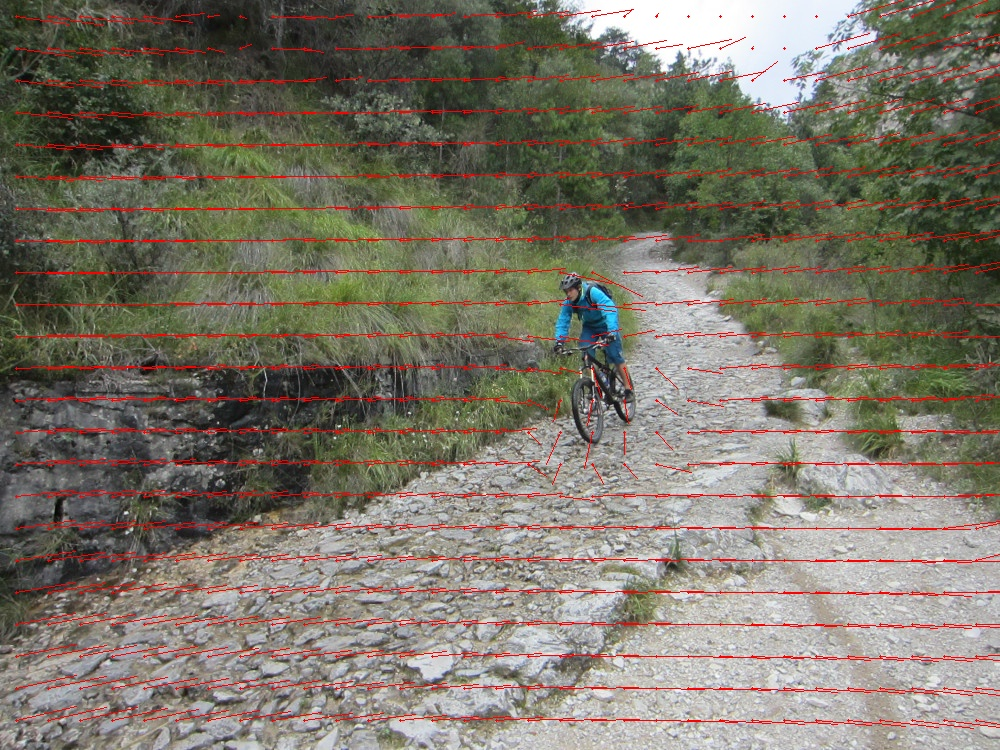
\includegraphics[width=0.9\textwidth]{02/of_vis2.jpg}
            \caption{Visualization of optical flow with vectors: the origin of the vector is shown by a small point (only a limited number of vectors are shown)}
    \end{subfigure}
    \caption[Optical flow visualizations]{Optical flow visualizations}\label{fig:of_vis}
\end{figure}

\subsubsection{Spherical Coordinate System}
too trivial?

\subsubsection{UV Coordinates for Spherical Geometry}
\begin{itemize}
  \item what are uv coordinates
  \item how can they be used for 360\degree images (mapping different projections)
\end{itemize}

\section{Related Work}
\begin{comment}
  
Image-based Rendering (IBR) and viewpoint interpolation started gaining interest with the advent of virtual walkthroughs, for example for Apple's QuickTime\textsuperscript{\textregistered} VR, in order to save render time by generating views from images instead of using complex 3D scenes including textures, lights and complex geometric models \cite{quicktime}.

Chen et. al., in their survey on image-based rendering \cite{survey2004} use the terms \emph{source description} and \emph{appearance description} to compare these basic rendering techniques: ``Traditional'' rendering techniques use \emph{source description}, i.e. the scene is described by the objects within it, their positions and properties. On the other hand, IBR techniques try to achieve the same goal through \emph{appearance description}. Vision itself has little to do with 3D geometries, it is the processing of a dense set of light rays by the brain which are captured through the eye. This process can also be synthesized by a capture device like a camera. So, instead of trying to describe the scene through the objects it contains, IBR rendering techniques try to model the \emph{light rays} that reach the viewer. 

A theoretical model for \emph{appearance description} was developed by Adelson et. al. \cite{Adelson91}: the \emph{plenoptic function} (Equation~\ref{eq:plenoptic}). The plenoptic function is a 7D function that describes the observable light at every point in space $V_x$, $V_y$, $V_z$, from every direction $\theta$, $\varphi$, at every wavelength $\lambda$, at every possible point in time $t$.

\begin{equation}
  \label{eq:plenoptic}
  P = P(\theta, \varphi, \lambda, t, V_x, V_y, V_z)
\end{equation}

In practice, it is unfeasible, if not impossible, to cover all dimensions of this function, as this would require a capture device at every location, at every point in time, capturing light rays coming from every direction. However, by making assumptions, IBR techniques try to reconstruct simplified versions of the plenoptic function. Depending on which assumptions are made and how the surroundings are sampled, varying requirements are met and different results are achieved.

Chen et. al. summarize these different types of assumptions in their survey \cite{survey2004} and categorize different techniques by their use of these assumptions. The first 

Shum et. al. \cite{survey2000} break different image-based rendering approaches down by categorizing how much geometry is used.  

Many of these approaches however, do use some geometry information in order to recalculate image points. The scene geometry is hereby either meticulously recorded at the time of the image capture, as with Kanade et. al's 3D Dome \cite{geometry97}, or inferred from the image data alone, 

The approach presented in this thesis is \emph{pixel-based}, i.e. using no geometry information, so the following section will first outline research aiming to synthesize viewpoints with the use of little to no geometry. Since the majority of pixel-based rendering research uses planar images, the second part will focus on research using 360\degree images, including approaches using geometry.

\begin{itemize}
  \item type of warping: uv mapping, warping based on triangulation and homography
  \item image representation: cube, planar, sphere
  \item constraints? color / angle / \ldots
  \item geometry? sparse, dense, none
  \item correspondences needed? sparse, dense, none
  \item type of input: planar, 360, 180 pano
  \item type of output: planar, 360, 180 pano
\end{itemize}

\subsection{Image Synthesis without 3D Geometry for Planar Images}

\end{comment}
\subsubsection{Megastereo \label{subsec:megastereo}}
\begin{comment}
correspondences needed: dense, geometry: none, constraints: angle?, image rep: planar, type of warping: none, because planar
Richardt et. al. \cite{megastereo} use a combination of image stitching and their own optical flow-based blending algorithm in order to create high resolution stereo panoramas from a set of planar images captured on a radius. The goal is to synthesize stereoscopic viewpoints (an image for the left and right eye, each) from the captured monoscopic images. After transforming the images so that they all have scene-independent orientation and minimal distortion, strips of the captured images are extracted for each ``eye'' based on the best matching image ray (Figure~\ref{fig:megastereo-figure}a and b). In cases where there is no perfect ray correspondence, the ray with the smallest deviation angle can be chosen, however, this can lead to artefacts as illustrated in Figure~\ref{fig:megastereo-figure}c. In order to mitigate these artefacts, Richardt et. al. introduce a blending algorithm based on optical flow: 

In order to blend two images, they take the two closest viewpoints $I_K$ and $I_L$ and interpolate $\widetilde{I_M}$ using the optical flow vectors $F_{k\rightarrow l}$ and $F_{l\rightarrow k}$.  The corresponding strip is then taken from this new viewpoint which contains the matching ray (Figure~\ref{fig:megastereo-figure}d).

\begin{figure}[]
\centering
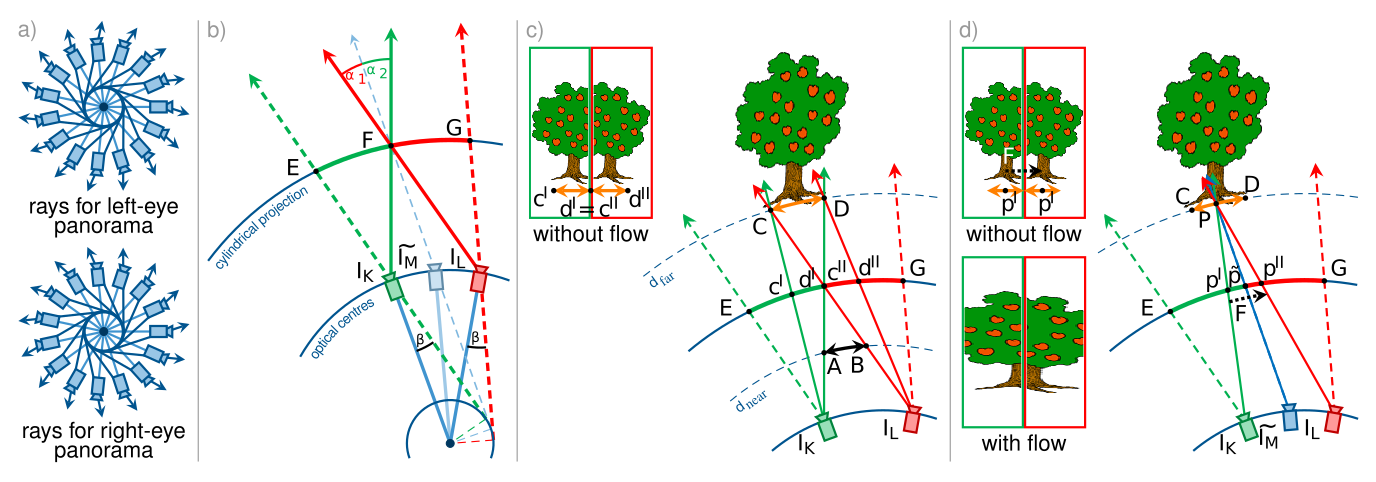
\includegraphics[width=1\textwidth]{02/megastereo-figure.png}
\caption[Flow-based blending in Megastereo]{(a) Illustration of rays required for creating a stereoscopic panorama and (b) deviation angle $\beta$. (c) Duplication and truncation artefacts caused by the aliasing. (d) Flow-based upsampling to synthesize required rays. \emph{From \cite{megastereo}}}
\label{fig:megastereo-figure}
\end{figure}

For Megastereo, there is no need to blend the complete images, instead, they restrict their calculations to the strips/pixels they need. For simplicity's sake, the process is described for a full image:
The interpolated image $\widetilde{I_M}$ at point $\alpha$ between the images $I_K$ and $I_L$ is calculated by shifting $I_K$ by $\alpha \cdot F_{k\rightarrow l}$ and by shifting $I_L$ by $(1 - \alpha) \cdot F_{l\rightarrow k}$. The two shifted images are then blended linearly, using $\alpha$ as the weight.

\begin{itemize}
  \item other approaches, such as light field approaches or neural network approaches
\end{itemize}

\subsection{Image Synthesis for 360\degree Images}

\subsubsection{6-DOF VR Videos with a Single 360-Camera}
correspondences needed: none, geometry: dense, constraints: none, image rep: cube, type of warping: triangulation
Huang et. al. \cite{6dof} propose a method to expand regular 360\degree video data into stereoscopic video data viewable with six degrees of freedom. Their approach is based on reconstructing the 3D scene and the camera path.

This reconstruction is achieved by adapting well-established structure-from-motion (SfM) algorithms for 360\degree data. Since SfM algorithms are designed for planar images with a limited field of view (FoV), the six separate faces of the cube map representation are used as input for the SfM algorithm. SfM algorithms work by tracking points across a series of images (e.g. frames), so for cube mappings, potential points moving across seams need to be accounted for. This is done by extending the field of view of each face so that regions around seams are represented on both sides of the seam. After the points are correctly tracked, the extended cube map is reduced back to its original format.

Then, the sparse scene geometry and camera path are calculated by incrementation and interpolation. The sparse geometry is then refined to a dense reconstruction of the scene using depth maps and Delaunay Triangulation. Finally, new viewpoints are synthesized by warping the current frame. Their warping algorithm projects the dense 3D points to a unit sphere control mesh with icosahedral tesselation\footnote{Icosahedral tesselation of a sphere subdivides the surface of a sphere into triangles. Other terms for this type of sphere are Icosphere or Geodesic Polyhedron} for both the captured viewpoint and the desired viewpoint. Then the vertex motion between each pair of triangles is calculated and the image warped according to these motion vectors (see Figure~\ref{6dof-figure}). 

\begin{figure}[]
\centering
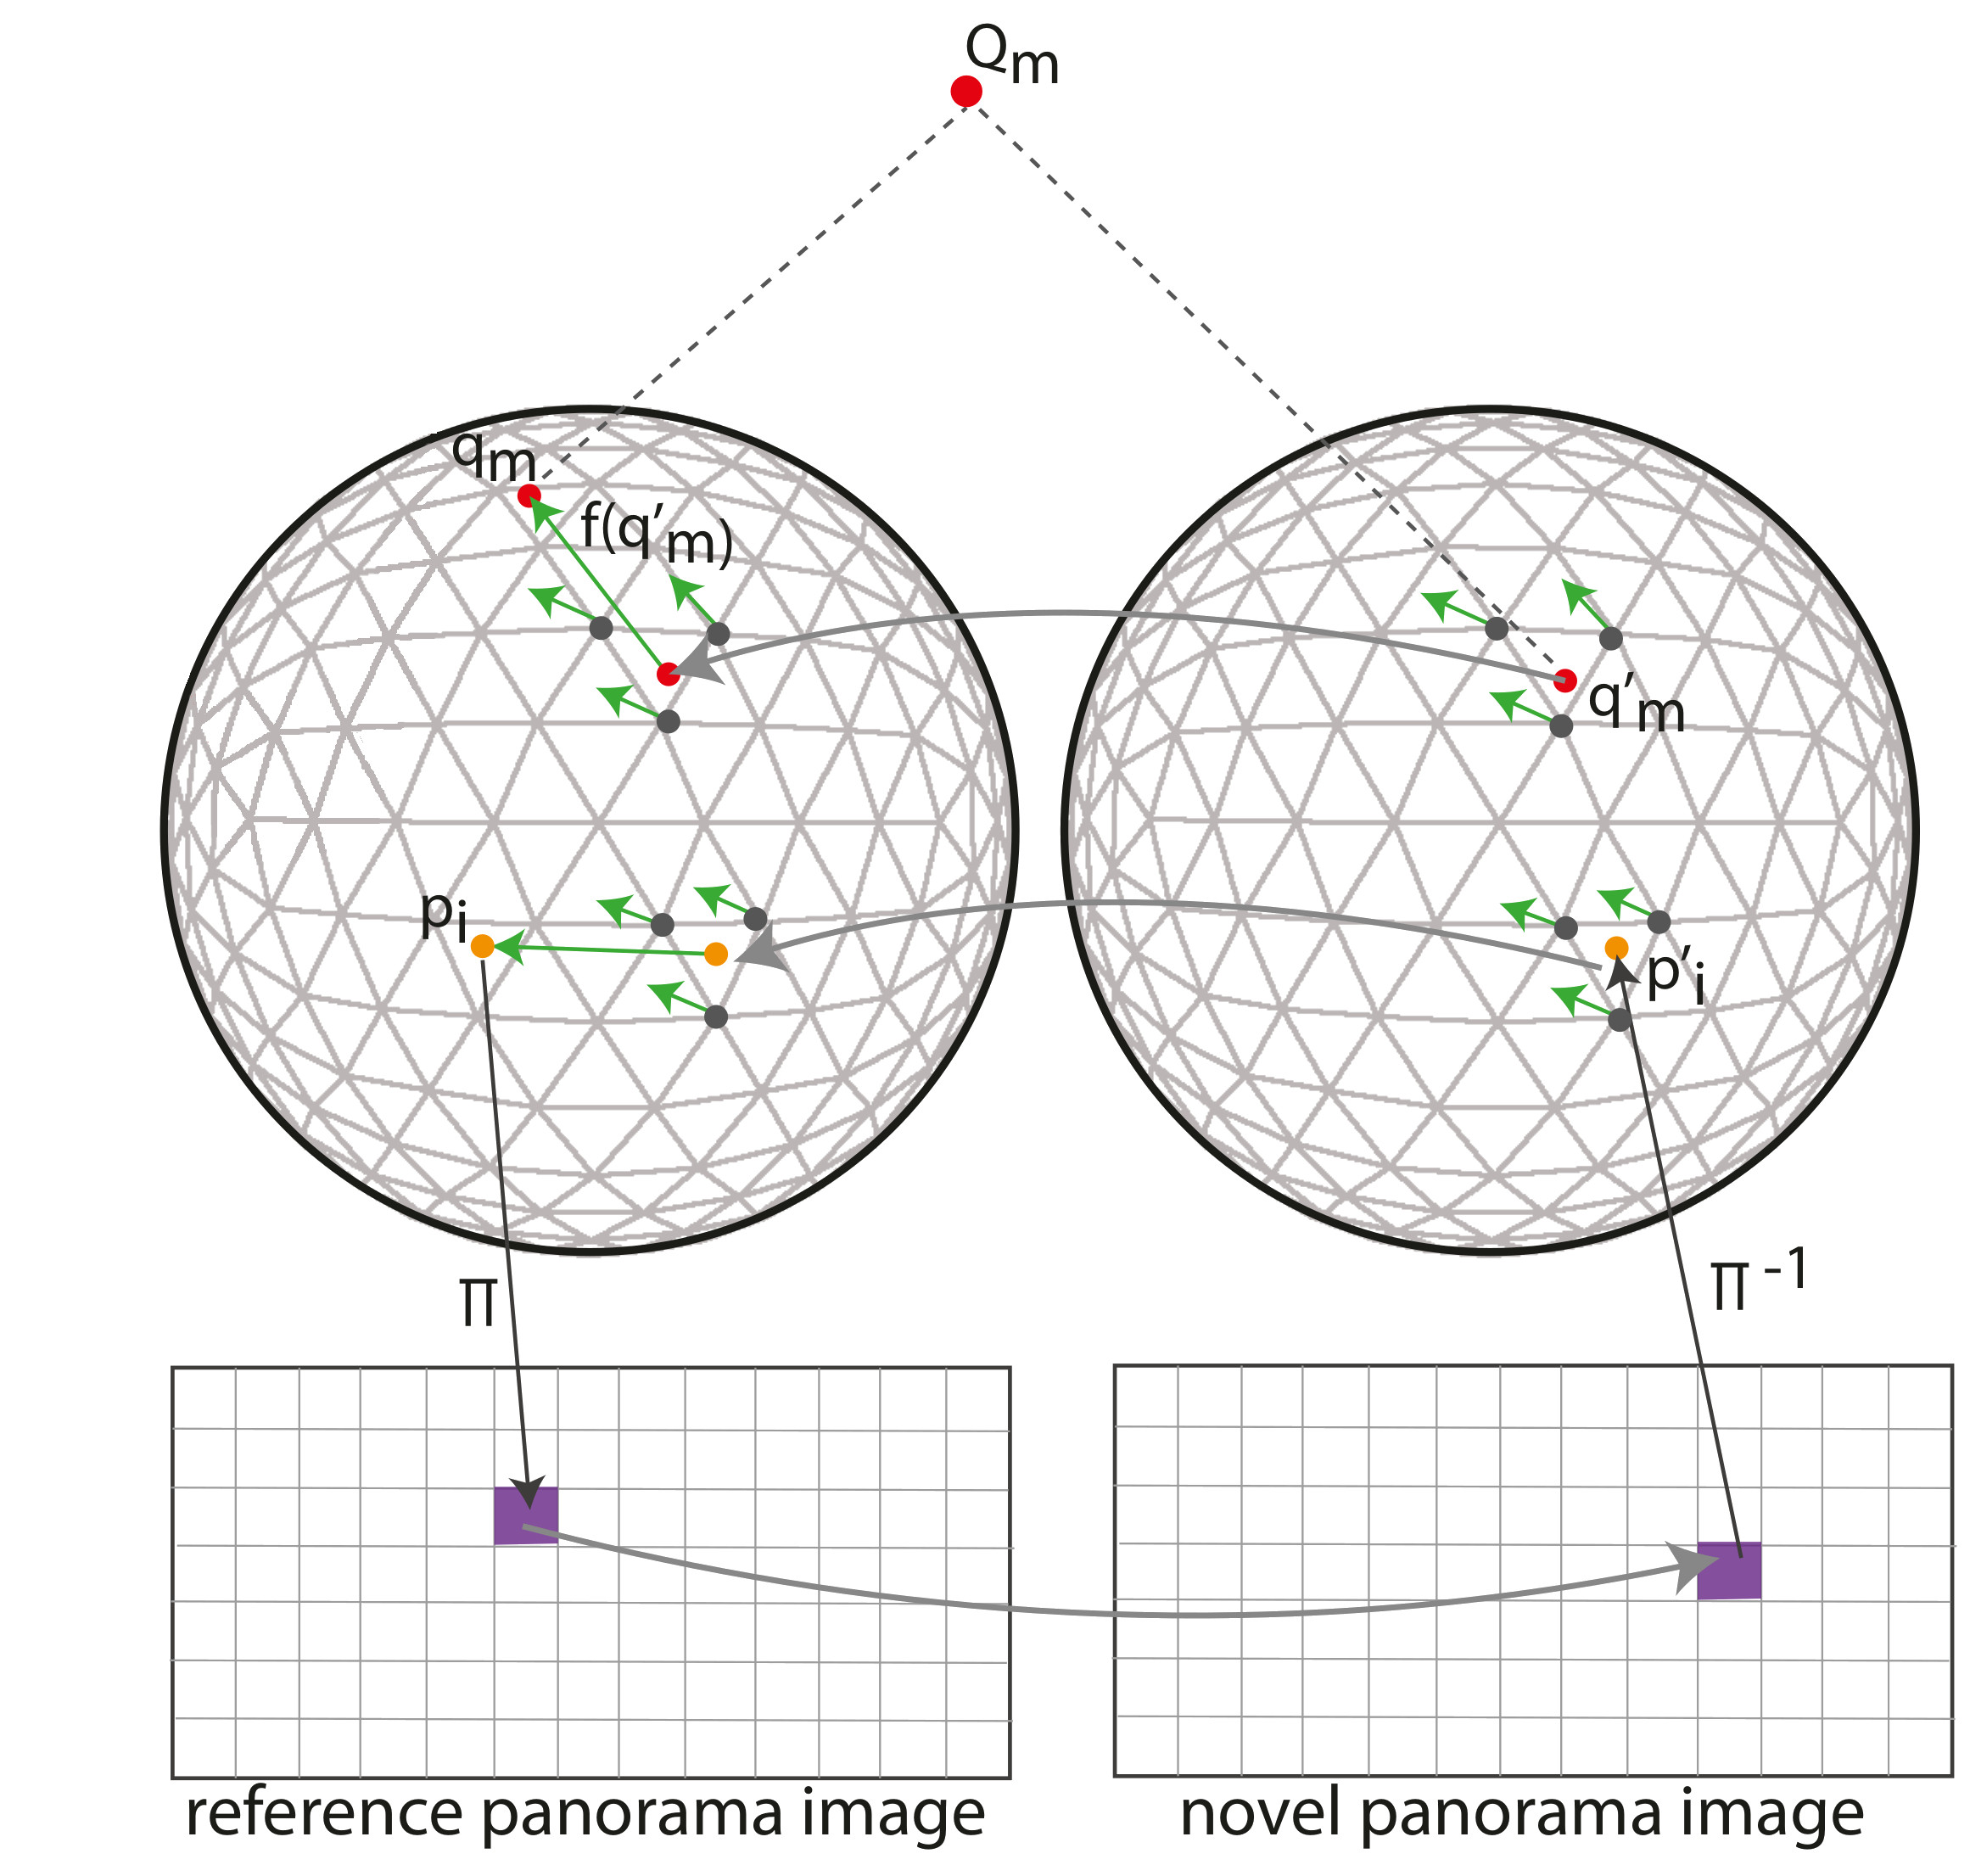
\includegraphics[width=0.6\textwidth]{02/6dof-figure.jpg}
\caption[Image warping from Huang et. al.]{The warping field is computed by finding the movement between the projections of each 3D scene point in the reference and the synthesized frame. Then the warping field is used to map each pixel of the synthesized image to its corresponding pixel in the reference to look up its color information. \emph{Adapted from \cite{6dof}}}
\label{fig:6dof-figure}
\end{figure}

\subsubsection{Panorama Image Interpolation for Real-time Walkthrough}
correspondences needed: sparse, geometry: none, constraints: none, image rep: ?, type of warping: triangulation
Kawai et. al. \cite{walkthrough} approach the problem of interpolating between images without using 3D geometry. Their basic setup is to capture four 360\degree images at each corner of a rectangular area and use their algorithm to interpolate within this area.

First, they manually select corresponding feature points in all four images, which they map to a sphere and triangulate. They create their synthesized mesh with bilinear interpolation, in which the triangulated meshes are deformed by using the Slerp (Spherical Linear Interpolation) function. To calculate the actual image, they use a combination of ray tracing and barycentric coordinates to get the uv coordinates of the synthesized image. Finally, the new image can be rendered by using the uv coordinates for texture mapping.

\subsubsection{On the Use of Ray-tracing for Viewpoint Interpolation in Panoramic Imagery}
correspondences needed: none, geometry: none/dense, constraints: color-constraint, image rep: cube, type of warping: pixel blending
Shi et. al. \cite{raytracing} examine how ray tracing can be used to calculate arbitrary new viewpoints based on knowledge of relative positions between the viewpoints which are stored as cube maps. For every pixel in the target image, a ray is cast into the scene. At the point where the ray intersects with the scene, the rays from the reference images that also intersect with the scene at the same position, are calculated, yielding the corresponding point in the reference images.

Shi et. al. introduce a color consistency constraint, which determines whether the pixel values of the reference images are similar. In areas where N reference images result in different colors, the pixel with the largest deviation is eliminated and the synthesized pixel is based on N - 1 reference pixels.

In order to calculate an intersection with the scene, they propose two different methods: A brute-force depth search which searches along the ray until the pixel values are similar enough to fulfill their color constraint requirements, or a guided depth search using sparse 3D reconstruction.

\subsubsection{Cube2Video: Navigate between Cubic Panoramas in Real-Time}
angular error metric
\end{comment}

    %\chapter{Proof of Concept Design and Implementation}
%\chapter{Pixel-based Synthesis of 360\degree Viewpoints}
\chapter{Pixel-based Synthesis of 360\degree Viewpoints with 2DoF}\label{chap:implementation}

%\ldots The different appraches to image-based rendering presented in the previous chapter use different assumptions and simplifications of the plenoptic function in order to facilitate its reconstruction. Most of these approaches are based on planar images, which already significantly reduces the complexity of the data to be processed. The approach presented here, on the other hand, works on 360\degree images, which increases data processing and storage. As a result, other assumptions and simplifications are made, the most prominent being the exemption of scene geometry, and the limitation to two degrees of freedom (2DoF). Limiting movement to 2DoF means that the location of possible synthesized points is restricted to a plane. 
\todo{lead into approach by outlining the method in comparison to related work}

This chapter presents the assumptions and simplifications made for the pixel-based synthesis of 360\degree viewpoints, the basic approach and an improvement to the basic approach based on flow-based blending from Richardt et al.'s Megastereo \cite{megastereo}, and the implementation details of the method.

\section{Approach} \label{sec:approach}
\todo{missing: intro to section}
%\begin{itemize}
%  \item most other approaches rely on either geometry or correspondences
%  \item usually some form of triangulation
%  \item use of sphere for ray tracing, then use texture lookup to find the pixel values
%  \item combination of reprojection ie warping with angle constraint and flow-based blending
%  \item first part relies on radius/scale, but no geometry, second part relies on image correspondences
%  \item ``view-dependent texture maps'' \ar environment map / viewpoint is chosen based on some kind of proximity to the synthesized view
%  \item pixel-based, in that each pixel is calculated separately, there are not image-area based constraints
%\end{itemize}

\subsection{Assumptions}
In order to simplify the process of synthesis, some assumptions are made based on the scene and the viewpoints in the scene:

\begin{itemize}
  \item the scene is static
  \item all images are captured on a plane parallel to the floor (viewpoint plane)
  \item all synthesized viewpoints are located inside the scene boundaries and are also located on the viewpoint plane
  \item the positions and orientations of the captures are known
  \item the scale (max radius) of the scene is known
\end{itemize}

Furthermore, for the moment, it is assumed that the optical flow algorithm used in the flow-based blending calculates a decent result between any pair of viewoints.

\subsection{Basic 2DoF Synthesis} \label{subsec:basic-synthesis}
With these assumptions and using a basic model geometry with approximately the same scale as the captured scene, it is already possible to synthesize new viewpoints with varying accuracy, depending on the scene. The process presented here for basic 2DoF synthesis is a combination of texture lookup through raytracing, and mosaicking by using a constraint based on the ray deviation angle.

\subsubsection{Raytracing-based Texture Lookup}
The first step is to map the texture (i.e. pixel values) of an existing viewpoint to a new viewpoint according to its position in the scene. Theoretically, any 360\degree viewpoint can be mapped to any other, since each 360\degree image captures each point in the scene. This is only theoretically the case, since image resolution and occlusions in the scene will conceal some areas for some viewpoints whereas they are visible for others. However, at this point, this will be ignored and it will be assumed that each viewpoint image contains all the points of the scene albeit at different image coordinates and different sampling rates\footnote{By design, areas closer to the camera are captured with a higher sampling rate per point than areas farther away.}. 

Additionally, 3D geometry of the scene is needed for raytracing. However, since the approach in this thesis does not capture or infer any real geometry, a model geometry is used that has approximately the same scale as the scene that was captured. The model geometry is a sphere, as this is a simple, very general geometry to represent a variety of different scenes. The radius of the sphere is chosen so that the sphere contains all possible points in the scene, for which the scale of the scene needs to be known. Under these assumptions, it is possible to map the image at one viewpoint to a new position by combining raytracing and texture lookup.

% This is visualized in Figure~\ref{fig:reflected_rays} a: Each point P of the scene reflects light rays in all directions. These light rays are captured at different viewpoints and are discretized into pixels in the image taken at that viewpoint. As a result, the pixels representing point P are present in the images captured at each viewpoint. This means that when synthesizing a new viewpoint S, the pixels representing point P can theoretically be retrieved from any of the images at the captured viewpoints (Figure~\ref{fig:reflected_rays} b).
%\begin{figure}[]
%\centering
%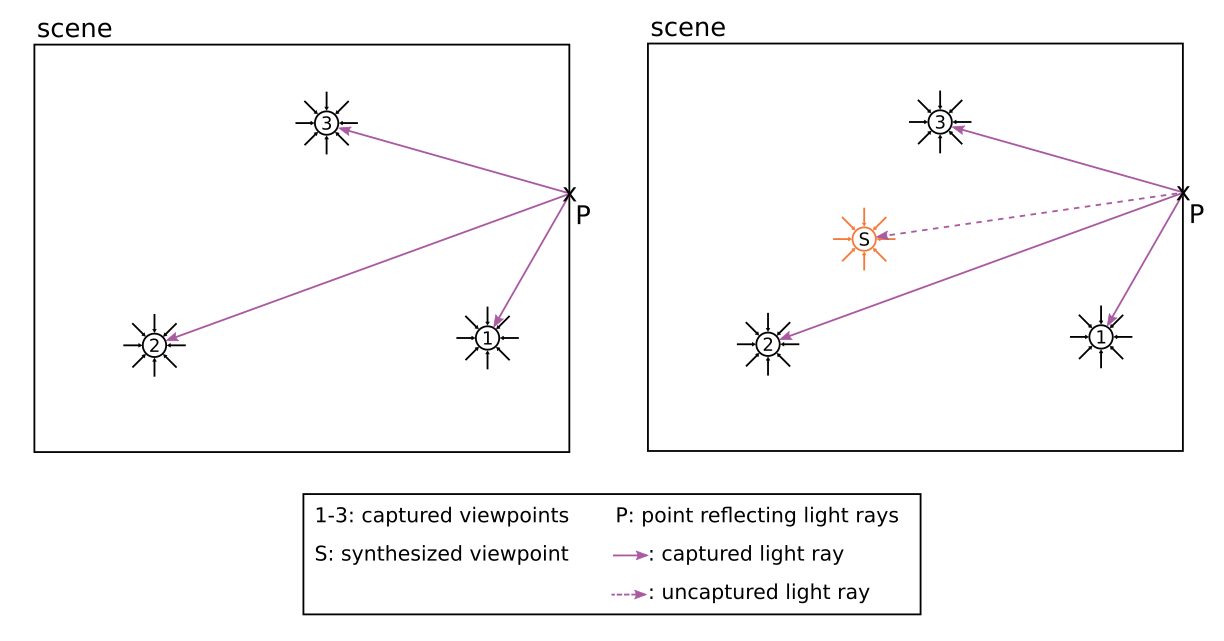
\includegraphics[width=1\textwidth]{03/incoming_lightrays.png}
%\caption[Light rays reflected from a point in the scene]{The reflected light rays from each point in the scene are captured by each 360\degree viewpoint}
%\label{fig:reflected_rays}
%\end{figure}

In order to do this, several steps of raytracing are necessary, which are visualized in Figure~\ref{fig:raytracing}. Figure~\ref{fig:raytracing}a shows how a camera at a specific viewpoint captures the light rays reflected from the objects in the scene. The captured pixel values are visualized on a circle around the center of projection of the camera (for simplicity's sake, only one row of pixels is shown). Once the viewoints have been captured (there is only one viewpoint in this example), a new viewpoint is ready to be synthesized. The model geometry is visualized as a circle\footnote{In this example, the model sphere does not surround the complete scene (the corners of the scene are outside of the circle). This is only for visualization purposes, normally the sphere would contain the complete scene, including the corners.} in Figure~\ref{fig:raytracing}b, with the new viewpoint to be synthesized represented by a dotted circle around a center of projection. For each pixel of the synthesized image, a ray is projected into the scene (Figure~\ref{fig:raytracing}c) and its intersection with the scene is calculated. Then, the ray from the center of projection of the captured viewpoint to the scene intersection is calculated, which, when normalized, is equivalent to a unit direction vector of the unit sphere. Using the unit direction and the image mapping function, the pixel value at that position is retrieved (Figure~\ref{fig:raytracing}e) and copied back to the new viewpoint (Figure~\ref{fig:raytracing}f). This way, the pixel values (i.e. texture) of a captured viewpoint are mapped to the new viewpoint (Figure~\ref{fig:raytracing}g). Figure~\ref{fig:raytracing}h compares the mapped values to the actual scene. It is immediately visible that most points have the value they would have, had the viewpoint been captured instead of synthesized (ground truth value), whereas some are incorrect. This is due to the disparity between the model and the real scene.

\begin{figure}
\centering
    \hfill
    \begin{subfigure}[t]{0.3\textwidth}            
            \centering
            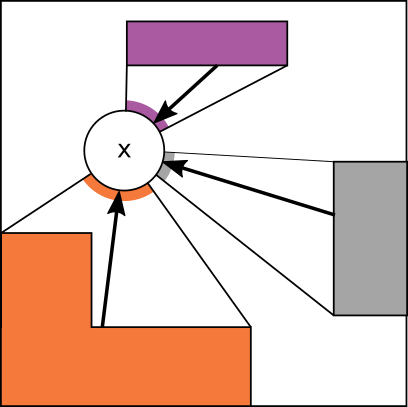
\includegraphics[width=0.9\textwidth]{03/raytracing01.png}
            \caption{The real scene viewed from above: The camera captures light rays reflecting from objects}
    \end{subfigure}%
    \hfill
     %add desired spacing between images, e. g. ~, \quad, \qquad etc.
      %(or a blank line to force the subfigure onto a new line)
    \begin{subfigure}[t]{0.3\textwidth}
            \centering
            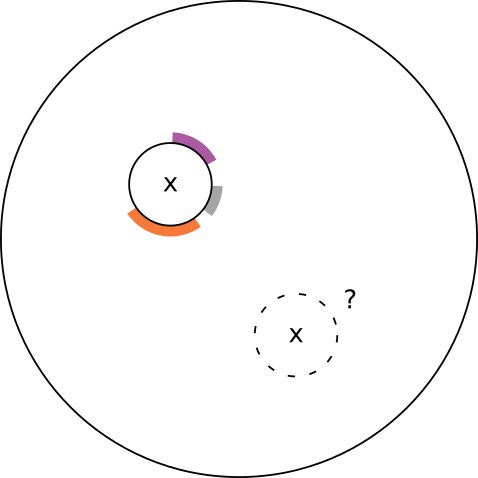
\includegraphics[width=0.9\textwidth]{03/raytracing02.png}
            \caption{A new viewpoint to be synthesized using the model geometry (sphere)}
    \end{subfigure}
    \hfill
    \hfill

    \hfill
    \begin{subfigure}[t]{0.3\textwidth}            
            \centering
            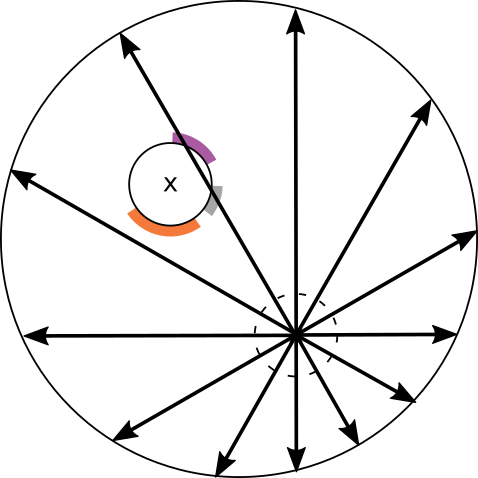
\includegraphics[width=0.9\textwidth]{03/raytracing03.png}
            \caption{A ray for each pixel in the synthesized viewpoint is traced to its intersection with the model}
    \end{subfigure}%
    \hfill
    \begin{subfigure}[t]{0.3\textwidth}
            \centering
            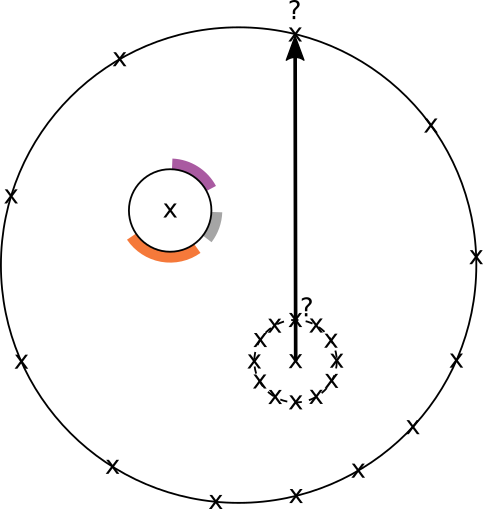
\includegraphics[width=0.9\textwidth]{03/raytracing04.png}
            \caption{For each ray, a texture lookup is performed}
    \end{subfigure}
    \hfill
    \begin{subfigure}[t]{0.3\textwidth}
            \centering
            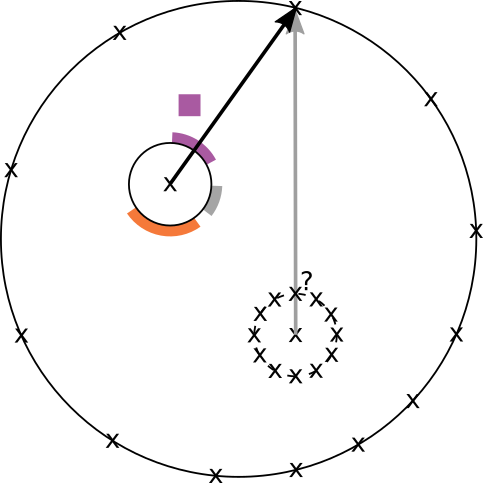
\includegraphics[width=0.9\textwidth]{03/raytracing05.png}
            \caption{From the ray-model intersection, a second ray is traced to the center of projection of the captured viewpoint and the pixel value is looked up}
    \end{subfigure}
    \hfill

    \hfill
    \begin{subfigure}[t]{0.3\textwidth}            
            \centering
            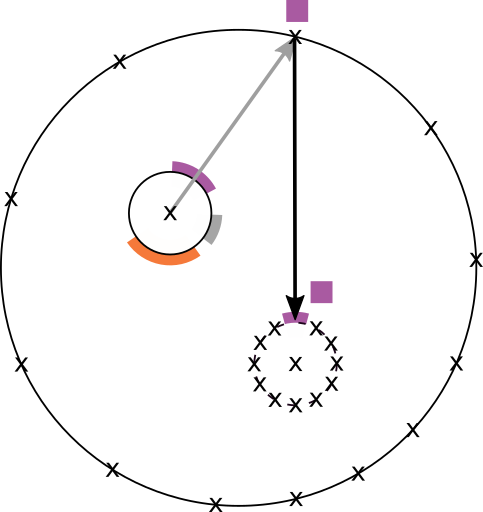
\includegraphics[width=0.9\textwidth]{03/raytracing06.png}
            \caption{The pixel value is copied back to the new viewpoint}
    \end{subfigure}%
    \hfill
    \begin{subfigure}[t]{0.3\textwidth}
            \centering
            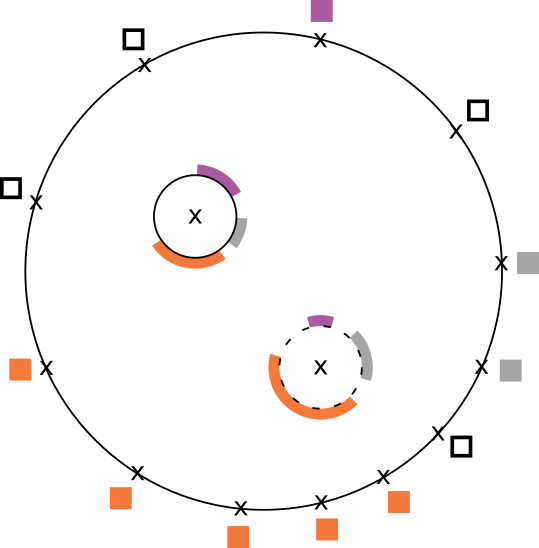
\includegraphics[width=0.9\textwidth]{03/raytracing07.png}
            \caption{This process is repeated for all pixels}
    \end{subfigure}
    \hfill
    \begin{subfigure}[t]{0.3\textwidth}
            \centering
            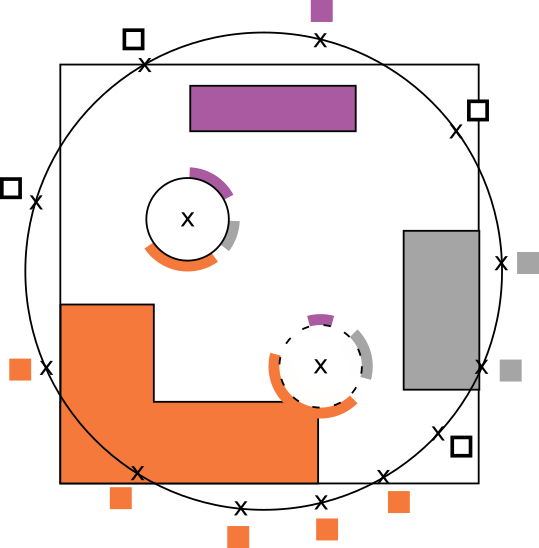
\includegraphics[width=0.9\textwidth]{03/raytracing08.png}
            \caption{The resulting texture mapping from the captured viewpoint to the model geometry in comparison with the original scene}
    \end{subfigure}
    \hfill
    \caption[Texture lookup through raytracing]{Process of texture lookup through raytracing}\label{fig:raytracing}
\end{figure}

%The basic idea of the 2/3DoF algorithm is to find the image areas from the set of existing viewpoints that are the ``most fitting'' for the synthesized viewpoint and transform these areas to approximate where they would be in the synthesized image. This means that a metric is necessary that measures how ``fitting'' a specific pixel of a viewpoint image is. Also, a reprojection needs to be found that transforms the ``fitting'' image areas to the appropriate image coordinates for the synthesized viewpoint.
%\missingfigure{point correspondences and reprojection intro}


\subsubsection{Deviation-angle-based Mosaicking}
The example in Figure~\ref{fig:raytracing} contains only one captured viewpoint, so the choice of which viewpoint to use for texture lookup is trivial. In cases where several viewpoints are available, a choice must be made as to which viewpoint should be used. In the case where the real scene has the same geometry as the model sphere, this is practically irrelevant, since the raytracing is always accurate. However, this is unrealistic, since the number of spherical rooms containing no objects is negligible. As a result, as soon as the real scene differs from the model sphere, some viewpoints yield better results than others. Figure~\ref{fig:dev_angle}a shows how a discrepancy between the real scene and the model sphere can lead to inaccurate results.

When comparing rays from different viewpoints, two metrics can be examined: the euclidean distance of the captured viewpoint from the synthesized viewpoint, and the deviation angle between the rays. Figure~\ref{fig:dev_angle}b visualizes the two metrics and in the example, the $vp2$ with the smaller deviation angle is a better match. In fact, assuming that there is no obscuring element in the air such as fog, and disregarding diffusion and scattering over distance, the same light ray is captured by any viewpoint located on the ray in question. This means the closer the deviation angle is to zero, the more accurate the result will be, no matter the distance of the viewpoints with the best result being a deviation angle of zero (Figure~\ref{fig:dev_angle}c). However, sampling rates and resolution also have an effect on the sampled point, so the euclidean distance cannot be completely ignored.

Instead of combining these metrics in a function that might have to be weighted differently depending on the scene size, the distribution viewpoints, and more, the choice of which viewpoints to use is divided into two different steps: The choice of input viewpoints from all captured viewpoints for the synthesis of a specific point, and the choice of which of the input viewpoints to use for each ray of the synthesized point. 

The pre-selection of input viewpoints from all captured viewpoints is based on the assumption that the closer the captured viewpoints are to the synthesized viewpoint, the more accurate the sampling of the surroundings will be (i.e. the relative size of the objects). As a result, all viewpoints further than a certain distance are discarded from the input. \label{misc:input_selection}

After selecting the most appropriate captured viewpoints, the synthesized image is created by comparing the deviation angles of these viewpoints for each ray (i.e. pixel). The two closest viewpoints are then blended together on a per-pixel basis, so that there are no abrupt edges between mosaic areas. The blending function is presented in more detail in Section~\ref{sec:impl_details}.
%depending on the number and relative location of the captured viewpoints, using a per-pixel, deviation-angle-based constraint leads to a synthesized image made up of patches from different viewpoints (i.e. mosaic). 

\begin{figure}
\centering
    \hfill
    \begin{subfigure}[t]{0.3\textwidth}            
            \centering
            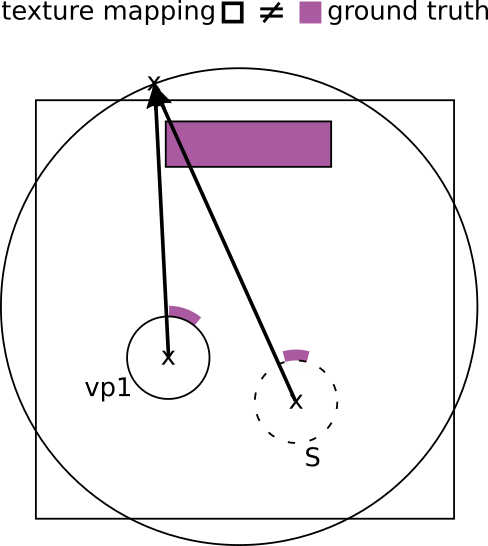
\includegraphics[width=0.9\textwidth]{03/dev_angles01.png}
            \caption{Differences in the real scene from the model can lead to inaccurate texture mappings}
    \end{subfigure}%
    \hfill
    \begin{subfigure}[t]{0.3\textwidth}
            \centering
            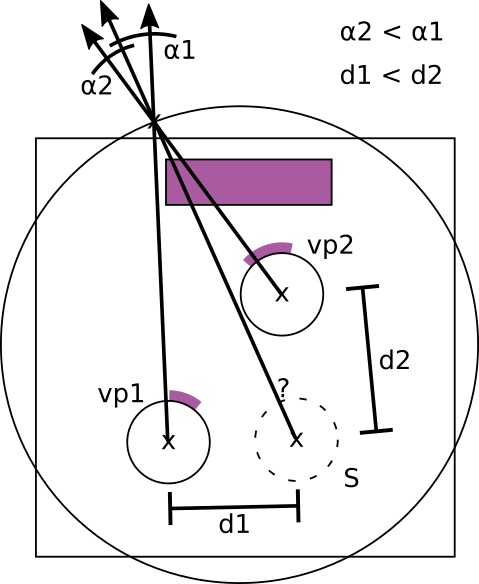
\includegraphics[width=0.9\textwidth]{03/dev_angles02.png}
            \caption{The deviation angle $\alpha$ of the rays can be compared, as well as the euclidean distance d}
    \end{subfigure}
    \hfill
    \begin{subfigure}[t]{0.3\textwidth}
            \centering
            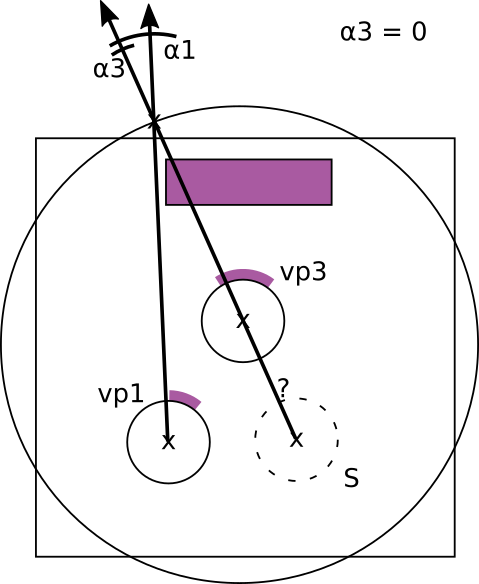
\includegraphics[width=0.9\textwidth]{03/dev_angles03.png}
            \caption{The optimal case (disregarding sample resolution) is when the deviation angle is 0, as for viewpoint 3 in this example}
    \end{subfigure}
    \hfill
    \caption[Choosing the appropriate viewpoint for texture lookup]{Choosing the appropriate viewpoint to improve the result} \label{fig:dev_angle}
\end{figure}
%In order to find the ``most fitting'' image area from all of the viewpoint images, there first needs to be a metric that measures how ``fitting'' an image area is. 

%One example is the euclidean distance of the viewpoint locations in space. This would mean that for each pixel, the corresponding pixel of the \emph{nearest viewpoint} would be used. This is the simplest approach, and would simply return the nearest neighbor. 

\subsection{2DoF Synthesis using Flow-based Blending}
Using basic 2DoF Synthesis works fairly well as long as the real scene geometry corresponds roughly to the model sphere. The basic shape of many rooms can be approximated by a sphere, however the objects within these rooms can diverge greatly from the model geometry. In these cases, ghosting and doubling artefacts become visible, such as areas appearing twice, not at all, or two areas overlapping inconsistently. This problem is exacerbated when the synthesized viewpoint is very close to an object, as is visualized in Figure~\ref{fig:flow-based-mot}: In this example the synthesized viewpoint is very close to a detailed object whose geometry diverges significantly from the model sphere. The values of the points captured by the two viewpoints $vp1$ and $vp2$ differ (orange and purple), and neither of them is the desired ground truth value (gray) (Figure~\ref{fig:flow-based-mot}a). In order to improve the result, an adapted variation of the flow-based blending method from Richardt et al.'s al.'s Megastereo \cite{megastereo} is introduced. This method allows interpolation between two 360\degree viewpoints using optical flow. Figure~\ref{fig:flow-based-mot}b shows how the interpolation can be used to achieve a more accurate result: A new viewpoint $vp$1-2 is interpolated between $vp1$ and $vp2$ such that the interpolated viewpoint is located on the ray in question\footnote{Positioning the interpolated viewpoint directly on the ray is only possible for rays that are on the 2D plane containing all the viewpoints. All other cases must be approximated.} This new viewpoint is then used for the texture lookup to create the synthesized image with the goal of improving the accuracy of the mapped point.

\begin{figure}
\centering
    \hfill
    \begin{subfigure}[t]{0.4\textwidth}            
            \centering
            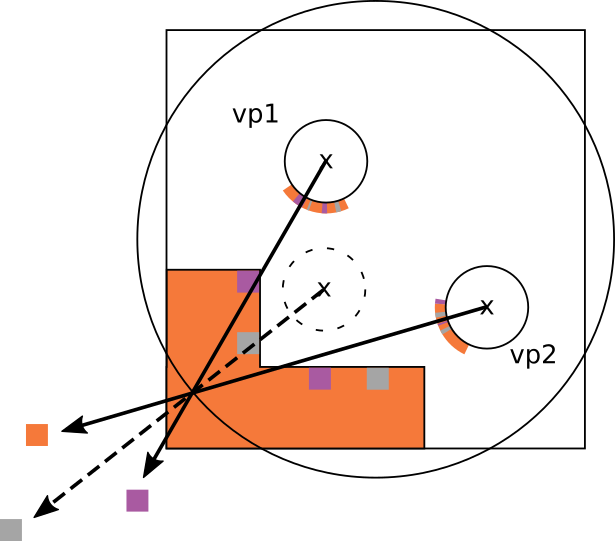
\includegraphics[width=0.9\textwidth]{03/flow-based01.png}
            \caption{Detailed areas where real geometry is very different from the model are problematic for basic 2DoF Synthesis}
    \end{subfigure}%
    \hfill
     %add desired spacing between images, e. g. ~, \quad, \qquad etc.
      %(or a blank line to force the subfigure onto a new line)
    \begin{subfigure}[t]{0.4\textwidth}
            \centering
            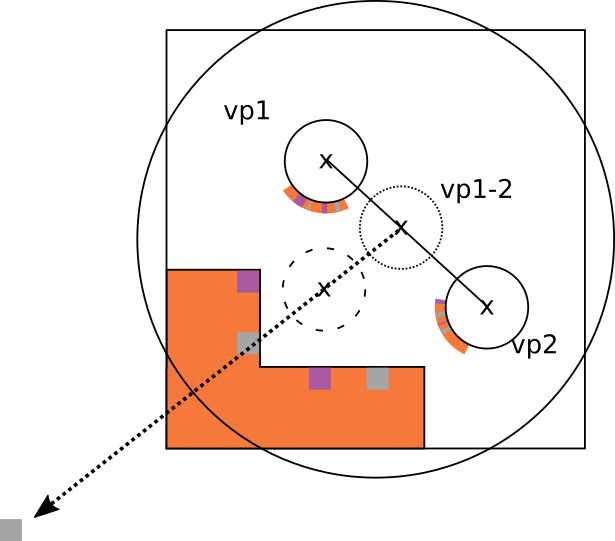
\includegraphics[width=0.9\textwidth]{03/flow-based02.png}
            \caption{Interpolating between input viewpoints using optical flow may improve results}
    \end{subfigure}
    \hfill
    \hfill
  \caption[Flow-based blending to improve accuracy in close, detailed areas]{Introducing flow-based blending to improve accuracy} \label{fig:flow-based-mot}
\end{figure}

%A solution to a similar problem has already been published by Richardt et al. in ``Megastereo'' \cite{megastereo} which introduces an approach using optical flow in order to reduce ghosting artefacts in planar images. The following section shows how the problem of 1D interpolation for 360\degree images can be reduced to the problem solved in Megastereo.

\subsubsection{Adapting Flow-based Blending in Megastereo for 1DoF Interpolation of 360\degree Images}
Megastereo \cite{megastereo} aims to generate high-resolution stereo panoramas by combining images captured on a circle. Their approach is to combine corresponding strips of the captured images and to create a view for each eye (see Section \ref{subsec:megastereo}). In order to mitigate artefacts such as ghosting, they use ``flow-based blending'' to combine two images A and B. This consists of using the optical flow vectors $F_{A\rightarrow B}$ and their inverse $F_{B\rightarrow A}$. To get the interpolated image at position $\delta$ between image A and B, first, image A is shifted by $\delta \cdot F_{A\to B}$ and image B is shifted by $(1 - \delta) \cdot F_{A\to B}$, yielding $I_A$ and $I_B$, respectively. Then, $I_A$ is multiplied by $(1-\delta)$ and $I_B$ by $\delta$ and these pixel values are added together to give the resulting interpolation. This is described by the following function, in which each pixel at position x of the synthesized image S is defined by: 

\begin{align}
S(x) &= (1-\delta ) \cdot A( x + \delta \cdot F_{A\to B}(x)) \nonumber\\
     &\qquad {} + \delta \cdot B( x + (1-\delta) \cdot F_{B\to A}(x)) \label{eq:flow_blending}
   \end{align}

%\subsubsection{Reducing 360\degree Interpolation to Planar Interpolation}
The flow-based blending in Megastereo operates on planar images. In order to use it for 360\degree synthesis, it is necessary to adapt the method for 360\degree images.

A 360\degree image can be projected in several ways, as described in Section \ref{subsec:fundamentals_360}. The output of these projections is a planar image, meaning that it would be possible to apply flow-based blending directly. However, optical flow algorithms are generally designed to handle planar images without seams or distortions and would most likely produce unexpected results if used naively on planar projections of 360\degree images. As a result, the 360\degree images must first be projected and adapted in such a way that optical flow can be calculated accurately on them.

%Most projections distort the image in some areas, which would result in distorted optical flow values, e.g. the areas towards the poles in the equirectangular projection. Furthermore, in order to make planar viewing possible, the 360\degree image must be ``unfolded'' along some seam. When calculating optical flow, points that move across the seam will not be tracked, even though they do not move out of the image space, as would happen in a regular image.

Of the projections presented in Section~\ref{subsec:fundamentals_360}, only the cube map representation is applicable. Spherical representations are impractical, as aligning seams is not feasible and the distortion towards the edges is extreme. The equirectangular representation has only four seams to handle, but also distorts the image greatly around the poles. The cube map representation contains a number of seams but does not distort the image more than a planar image would be. 
The challenge presented by the many seams of the cube map is to be able to track points that move across the seams created by the six faces. Figure~\ref{fig:flow_seams} shows an example of different points moving across seams, illustrating why calculating optical flow on each face separately would not be enough. Figure~\ref{fig:flow_seams} also shows the linear discontinuities at the seams (e.g. at the upper edge of the carpet): since each cube face was captured by a different virtual camera, angles are not consistent across seams. As a result it is not possible to use the cube map as it is, since the optical flow assumes linear movement\footnote{Optical flow uses vectors to describe movement, which are inherently linear}.

\begin{figure}
\centering
    \hfill
    \begin{subfigure}[t]{0.5\textwidth}            
            \centering
            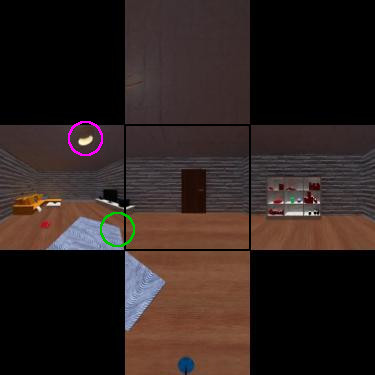
\includegraphics[width=0.9\textwidth]{03/flow_seams01.jpg}
            \caption{Viewpoint A in cube map representation (90\degree FoV per face)}
    \end{subfigure}%
    \hfill
     %add desired spacing between images, e. g. ~, \quad, \qquad etc.
      %(or a blank line to force the subfigure onto a new line)
    \begin{subfigure}[t]{0.5\textwidth}
            \centering
            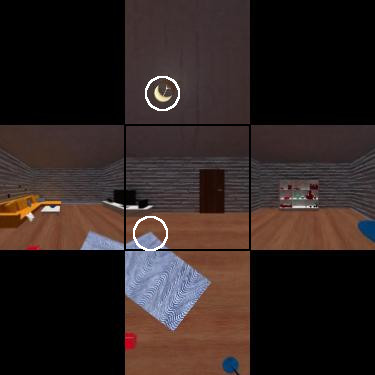
\includegraphics[width=0.9\textwidth]{03/flow_seams02.jpg}
            \caption{Viewpoint B in cube map representation (90\degree FoV per face)}
    \end{subfigure}
    \hfill
    \hfill
  \caption[Points traversing seams in the cube map]{Points in the scene moving across seam edges need to be tracked by optical flow (the back face of the cube map was omitted for simplicity's sake)} \label{fig:flow_seams}
\end{figure}

To solve this problem, an \emph{extended} cube map is introduced, which was also used by Huang et al.\ \cite{6dof} and Kolhatkar et al.\ \cite{360flowblending} to adapt 360\degree images for structure-from-motion algorithms. Instead of projecting a field of view of 90\degree for each camera, which covers exactly 360\degree of the image, the extended cube map uses a larger field of view for each camera (in this case, 150\degree). As a result, some areas of the scene are represented several times: the areas of the image that are near a seam are represented on each face that is adjacent to the seam. This way, when calculating optical flow on each face separately, points that move across where the seam would be in a regular cube map remain on the face with the corresponding projection. Figure~\ref{fig:flow_seams_ext} shows the front, top, and left faces of the extended cube map representation of the cube map shown in Figure~\ref{fig:flow_seams}. In the extended cube map, the tracked points do not traverse a seam on any of the faces, meaning optical flow can be calculated on the entire original face.

\begin{figure}
\centering
    \hfill
    \begin{subfigure}[t]{0.5\textwidth}            
            \centering
            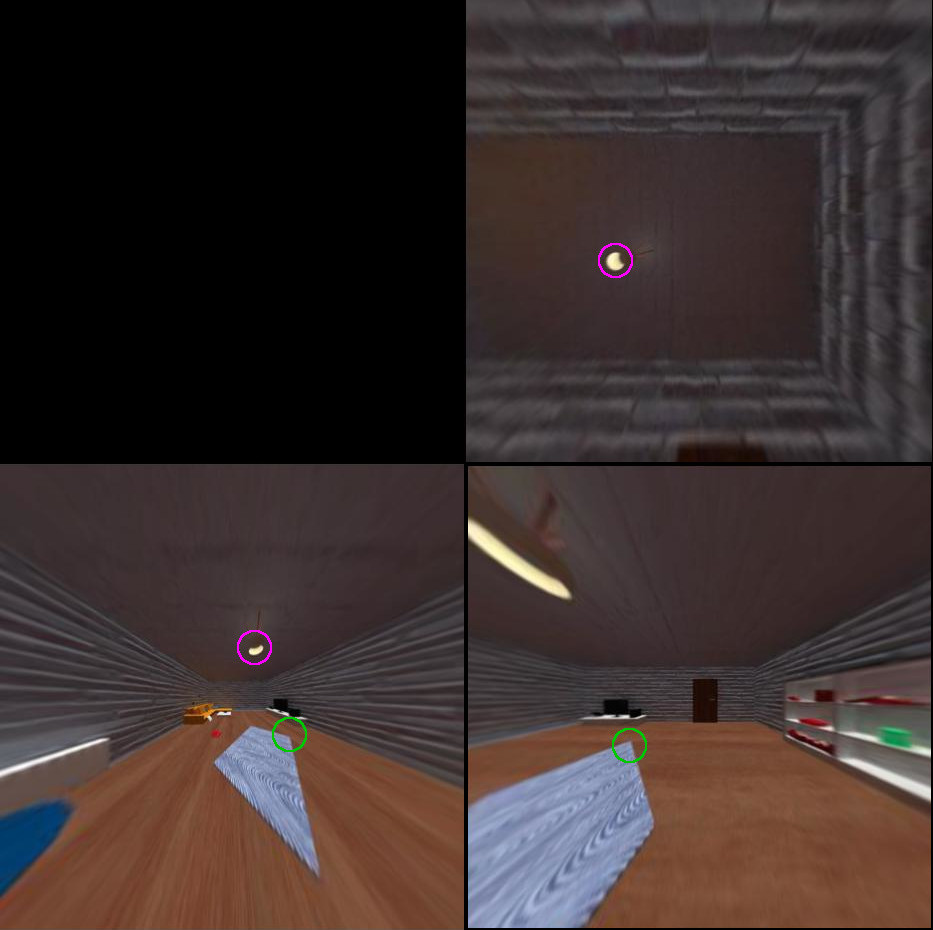
\includegraphics[width=0.9\textwidth]{03/flow_seams_ext16.jpg}
            \caption{Viewpoint A in extended cube map representation (150\degree FoV per face)}
    \end{subfigure}%
    \hfill
     %add desired spacing between images, e. g. ~, \quad, \qquad etc.
      %(or a blank line to force the subfigure onto a new line)
    \begin{subfigure}[t]{0.5\textwidth}
            \centering
            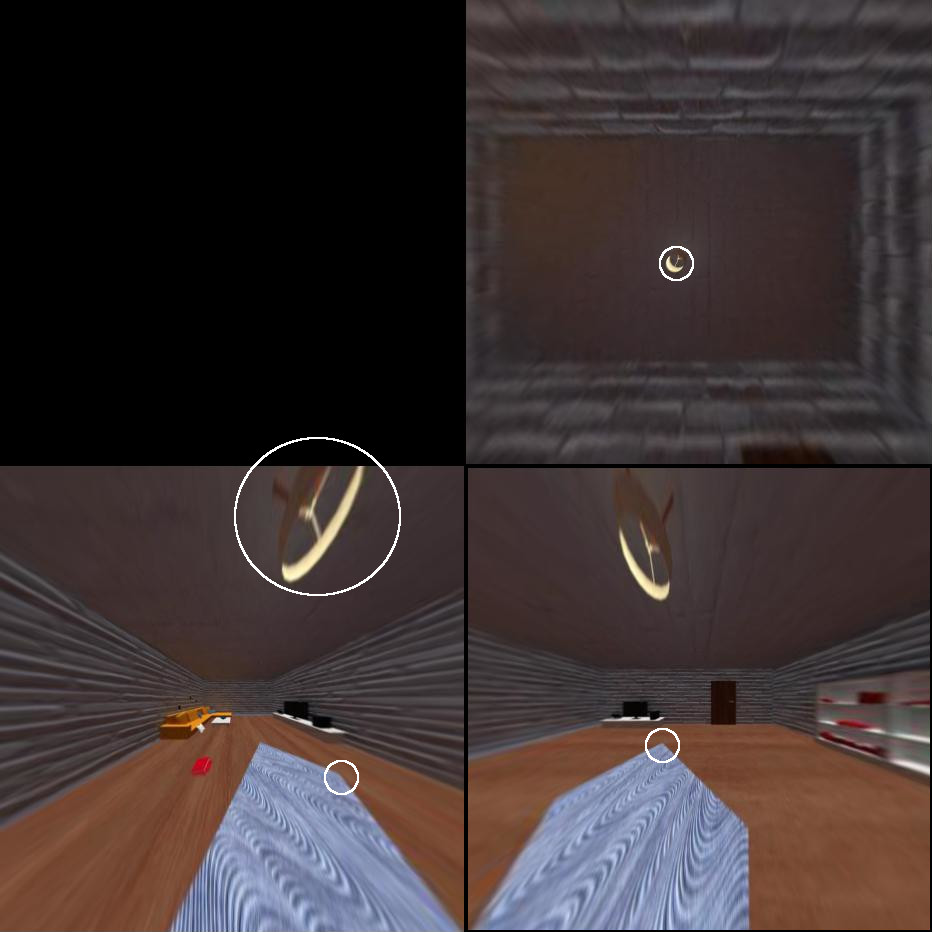
\includegraphics[width=0.9\textwidth]{03/flow_seams_ext15.jpg}
            \caption{Viewpoint B in extended cube map representation (150\degree FoV per face)}
    \end{subfigure}
    \hfill
    \hfill
  \caption[Tracking points across seams in the extended cube map]{Points that traversed a seam in the regular cube map can be tracked across the original seams in the extended cube map} \label{fig:flow_seams_ext}
\end{figure}

Nonetheless, this method is still limited by the field of view used by the virtual cameras. If the maximum displacement is larger than the face extension, the extended cube map will not be sufficient, as the points can also traverse the extended seams. Also, the larger the field of view, the more the image will be distorted towards the edges of a face, which may lead to distorted optical flow results. Both problems are visible in Figure~\ref{fig:flow_seams_ext}: The lamp in the left face has such a large displacement between a and b that it is partly cut off in b. On top of being cut off, it is also greatly distorted, which will result in distorted optical flow values for that area.

In general, this means that displacement between two images is limited. However, the displacement that is trackable by optical flow algorithms is also limited. The effect of these limitations will be explored in Chapter~\ref{chap:evaluation}.

Despite these limitations, using the extended cube map makes it possible to calculate optical flow on each face separately, meaning that Megastereo's flow-based blending method can be applied to two 360\degree viewpoints A and B: First, the extended cube map projections $A_{ext}$ and $B_{ext}$ are created from the image data. From this point, each set of faces $A_{ext}^{i}$ and $B_{ext}^{i}, i \in [top, left, front, right, bottom, back]$ is handled separately. Optical flow $F_{A\to B}^i$ and inverse optical flow $F_{B\to A}^i$ are calculated for $A_{ext}^{i}$ and $B_{ext}^{i}$. Then, the shifted image is calculated using Equation~\ref{eq:flow_blending}. Finally, for each face, the extended parts of the extended cube map are clipped so that each face once again has a field of view of 90$^{\circ}$, resulting in the blended 360\degree image at position $\delta$ between viewpoints A and B. Since the flow-based blending method is applied to two complete images instead of image strips like in Megastereo, it is equivalent to interpolation with one degree of freedom (i.e. on a line) between viewpoints A and B. This interpolated viewpoint can then be used for texture lookup just like a captured viewpoint.

\subsubsection{2DoF Synthesis with Flow-based Blending} \label{subsec:2dof_flow-based}
Adapting Megastereo's flow-based blending for 1DoF interpolation of 360\degree images allows the creation of a new viewpoint between A and B that is closer to the actual ray (Figure~\ref{fig:flow-based-mot}b). In order to leverage this to improve the basic 2DoF synthesis, the 1DoF interpolation needs to be integrated in the 2DoF synthesis algorithm. For each pixel of the synthesized image, a set of input viewoints A and B needs to be chosen for use in the 1DoF interpolation. Then, based on the positions of A and B, and the ray in question, an interpolation distance $\delta$ must be calculated that defines the position of the 1DoF interpolation between A and B.

For these steps, an approximation needs to be made due to the 2DoF restriction: Figure~\ref{fig:flow_simplification-mot}a and b show the ideal case, where the target point $T$ is on the same horizontal plane as the captured points and the synthesized point (the viewpoint plane). In this case there are a number of different positions directly on the ray that are also on the plane. Depending on the input viewpoints, the most convenient can be chosen and an interpolated viewpoint calculated at that position. However, this is only the case for all target points \emph{on this plane}. All other target points in the scene lie either above or below the viewpoint plane, for example in Figure~\ref{fig:flow_simplification-mot}c, where T is above the plane. In these cases, the only intersection of the ray and the viewpoint plane is at the synthesized viewpoint. Finding the set of viewpoints A and B that allow the closest 1DoF interpolation to this point is not trivial, as it would require comparing the minimum distance of the point to all vectors between all the possible sets of viewpoints. In order to simplify this problem, all the rays that are not on the viewpoint plane are approximated.

To approximate a ray pointing at target point T at the spherical coordinates $(r, \theta, \varphi)$, the elevation $\theta$ is reduced to 0, assigning the spherical coordinates to $(r, 0, \varphi)$, which is equivalent to moving T to the viewpoint plane by the shortest path. This will yield less accurate results as the actual ray moves towards the poles, since the deviation angle between the actual ray and the approximated ray increases towards the poles. However, this approximation is computationally and mathematically much simpler and should yield acceptable results.

\begin{figure}
\centering
    \hfill
    \begin{subfigure}[t]{0.3\textwidth}
            \centering
            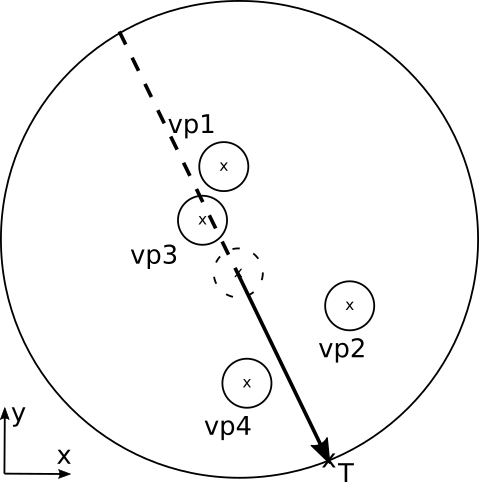
\includegraphics[width=0.9\textwidth]{03/flow_simplification01.png}
            \caption{Scene view from above: The target point T is on the viewpoint plane}
    \end{subfigure}%
    \hfill
    \begin{subfigure}[t]{0.3\textwidth}
            \centering
            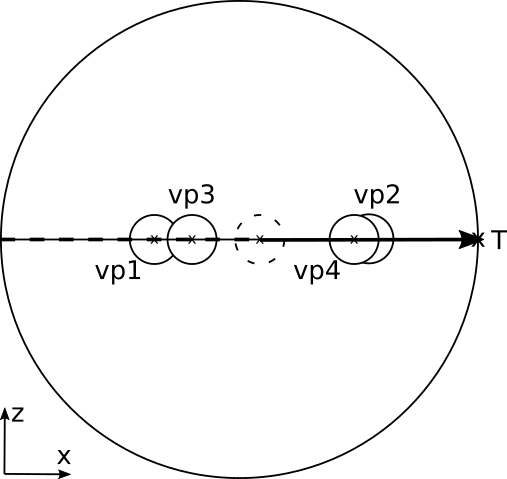
\includegraphics[width=0.95\textwidth]{03/flow_simplification02.png}
            \caption{Scene view from the side: The target point T is on the viewpoint plane}
    \end{subfigure}
    \hfill
    \begin{subfigure}[t]{0.3\textwidth}
            \centering
            
\includegraphics[width=0.9\textwidth]{03/flow_simplification03.png}
            \caption{Scene view from the side: The target point T can also be above (or below) the viewpoint plane}
    \end{subfigure}%
    \hfill
    \hfill
  \caption{Example of different target points in the scene} \label{fig:flow_simplification-mot}
\end{figure}

With this approximation, the viewpoints A and B used for 1DoF interpolation can be chosen. As in basic 2DoF synthesis, the metric for choosing A and B is the deviation angle. The actual rays, not the approximated rays, are used for the calculation and comparison of the deviation angles, since there is no need to use the approximated rays at this point. However, for the choice of A and B, an additional constraint is included: The two viewpoints chosen must be on either side of the approximated ray, so that there is an intersection between the vector connecting the viewpoints A and B and the approximated ray (see Figure~\ref{fig:flow_vpchoice}).

\begin{figure}
\centering
    \hfill
    \begin{subfigure}[t]{0.3\textwidth}
            \centering
            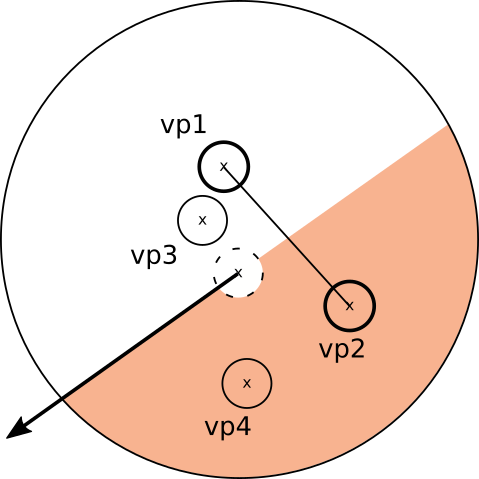
\includegraphics[width=0.9\textwidth]{03/flow-vpchoice01.png}
            \caption{A: vp1, B: vp2}
    \end{subfigure}%
    \hfill
    \begin{subfigure}[t]{0.3\textwidth}
            \centering
            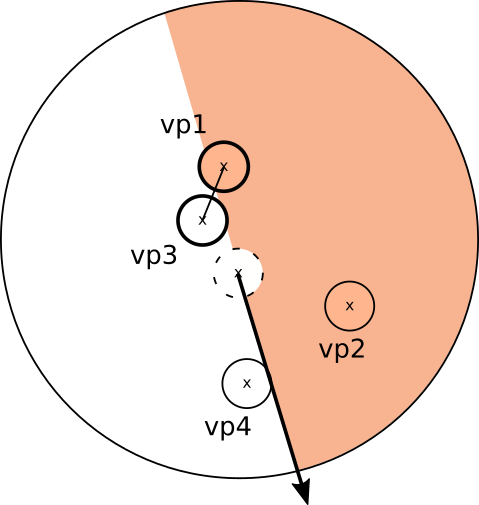
\includegraphics[width=0.9\textwidth]{03/flow-vpchoice02.png}
            \caption{A: vp1, B: vp3}
    \end{subfigure}
    \hfill
    \begin{subfigure}[t]{0.3\textwidth}
            \centering
            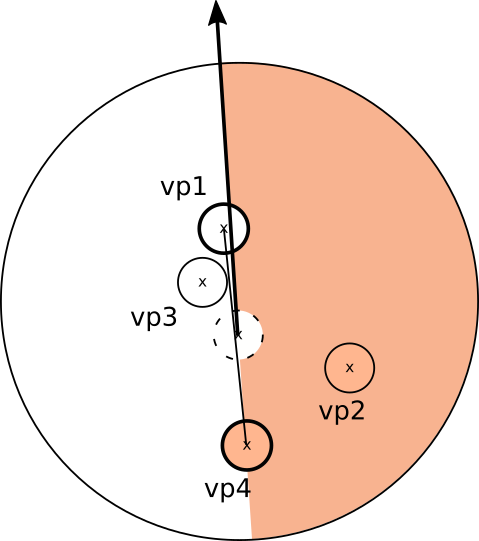
\includegraphics[width=0.9\textwidth]{03/flow-vpchoice03.png}
            \caption{A: vp1, B: vp4}
    \end{subfigure}%
    \hfill
    \hfill
  \caption[Examples of the choice of viewpoints A and B for 1DoF interpolation]{Examples of the choice of viewpoints A and B for 1DoF interpolation based on deviation angle and position on either side of the ray. The two sides of the ray are color coded in white and orange.} \label{fig:flow_vpchoice}
\end{figure}

Once the viewpoints A and B are chosen for each target point T, the interpolation distance $\delta \in [0,1]$ is calculated, which is the the point on the vector $\overrightarrow{AB}$ that intersects the approximated ray. The calculation of $\delta$ is a simple line intersection calculation, explained in Section \ref{sec:impl_details}.

Using the chosen viewpoints A and B, and the calculated interpolation distance $\delta$, a 1DoF interpolation is calculated for each approximated ray. Using this interpolated viewpoint, a texture lookup is then performed for each pixel associated with that ray. This results in a mosaicked image where each image area (vertical strip in equirectangular representation) is an interpolated, reprojected viewpoint. The 1DoF interpolation step should improve some of the artefacts caused by the use of the model sphere instead of the actual scene geometry. Its effectiveness and limitations are explored in Chapter~\ref{chap:evaluation}.

\section{Implementation Details} \label{sec:impl_details}
This section presents the technical and mathematical details on which the basic 2DoF synthesis and the 2DoF synthesis with flow-based blending are based. 
The basic 2DoF synthesis and the 2DoF synthesis with flow-based blending are implemented in Python3 \cite{python}, using the libraries NumPy \cite{numpy}, OpenCV \cite{opencv}, SciPy \cite{scipy}, and scikit-image \cite{skimage}. For the conversion between different 360\degree projections, as well as the calculation of the extended cube map, the library ``skylibs'' \cite{skylibs} is used.

\missingfigure{2DoF process diagram}

\subsection{Preprocessing}
The input data consists of a set of captured viewpoint images in equirectangular representation, a text file containing the metadata (positions and orientations) of these viewpoints, and the approximate scene radius. In order to easily and intuitively access the locations and image data of the captured viewpoints, the data is encapsulated in the CaptureSet class. The CaptureSet class first parses the metadata, then, with this information, rotates all the images so that they have the same orientation, and shifts the viewpoint cloud so that it is centered around the origin (0,0,0). This is done under the assumption that images were captured in a regular distribution throughout the room. The model sphere representing the scene is also centered at the origin. Instead of storing the image data directly in the CaptureSet, the file paths are stored so that the images can be dynamically loaded when needed. The CaptureSet can then be used by the ImgSynthesizer to synthesize a new image either using regular blending or flow-based blending at any given location within the scene\footnote{Given that it is within the convex hull of the captured viewpoints}.

\subsection{Basic 2DoF Synthesis}
For the basic 2DoF Synthesis, the steps described in detail in this section are the selction of input viewpoints, the calculation of the ray-scene intersection and the texture lookup, as well as the deviation angle calculation and blending function introduced in Section~\ref{subsec:basic-synthesis}.

\subsubsection{Selecting Appropriate Input Viewpoints}
Before calculating ray-scene intersections and performing texture lookup, the most appropriate input viewpoints are selected from the complete set of input viewpoints. In reality, resolution does play a role in the resampling, meaning that captured viewpoints that have a large euclidean distance from the synthesized viewpoint will not necessarily yield the ``correct'' value. Since the euclidean distance is not factored in to the weighting function (see~\pageref{misc:input_selection}), the captured viewpoints are filtered before synthesis. All viewpoints outside a certain radius (approx. 1m) are discarded. If the set of viewpoints within the radius is empty, all viewpoints are used, regardless of distance.

\subsubsection{Calculating Ray-sphere Intersection}
The ray-sphere intersection is used in the raytracing-based texture lookup to find the scene points captured by the synthesized viewpoint (see \ref{fig:raytracing}c). This raytracing process is a basic raytracing technique used in computer graphics. The vectors representing the rays of a viewpoint can be easily derived from the unit directions of the 360\degree image (see~Section~\ref{subsec:fundamentals_360}): Each unit direction is a vector on the unit sphere, representing the location of an image value (pixel). These coordinates are in \emph{model space}, meaning that they are centered around zero. Translating them into \emph{world space} moves the rays to their respective location in the scene, where the vectors represent the rays cast into the scene, where they will intersect with the model geometry.

The intersections of these rays with the model sphere can be calculated analytically: The model sphere, which is centered at the origin, can be represented implicitly by Equation~\ref{eq:rsi_spherefull}. The set of points P defined by this equation make up the surface of the sphere (Equation~\ref{eq:rsi_sphereP}). 
The equation describing any point on the ray can be expressed by Equation~\ref{eq:rsi_point}, where $O$ is the origin of the ray, which is the center of projection of the new viewpoint, $t$ is the length of the ray and $D$ is a unit vector describing the direction. 

\begin{align}
  x^2 + y^2 + z^2 - R^2 = 0&\label{eq:rsi_spherefull}\\ 
  P^2 - R^2 = 0&\label{eq:rsi_sphereP}
\end{align} 
\begin{align}
  P = O + tD& \label{eq:rsi_point}
\end{align} 

The point $P$ in Equation~\ref{eq:rsi_sphereP} can be substituted with the equation of the any point on the ray which yields Equation~\ref{eq:rsi_sub}. This equation can be developed into Equation~\ref{eq:rsi_quad}, which is a quadratic function with $a = D^2$, $b = 2OD$, $c = O^2-R^2$ (Equation~\ref{eq:quadf}).

\begin{align}
  |O + tD|^2 - R^2 &= 0  \label{eq:rsi_sub}\\
  D^2 t^2 + 2ODt + O^2 - R^2 &= 0 \label{eq:rsi_quad}
\end{align}

\begin{align}
  a = D^2, b = 2OD, c = O^2-R^2 \nonumber \\
  f(t) = at^2 + bt + c \label{eq:quadf}\\
  t = \frac{-b \pm \sqrt{b^2 - 4ac}}{2a} \label{eq:solvequadf}
\end{align}

This equation can then be solved for t. Since the radius of the sphere is chosen so that it contains the complete scene and no viewpoints are synthesized outside of the scene, the quadratic function will always have two solutions (i.e. two intersections): one for which the vector length $t$ is negative, and one for which the vector length is positive. Since the original ray used for the calculation is unidirectional (i.e. it cannot invert its direction), it needs to be extended by a positive value. The original ray, being a unit ray of length 1, can then be multiplied by the positive $t$, which yields the intersection point. 

The vectors and intersection points are each calculated and stored in latlong representation (i.e. matrix of vectors of the same shape as the latlong image), which means that they can handily be associated with the unit directions, as well as the uv coordinates (and thus, pixel values) using the latlong mapping function. By storing the values in this representation (i.e. 3D matrix), Numpy's vectorization can be used, which greatly facilitates implementation.

\subsubsection{Texture Lookup}
The texture lookup shown in Figure~\ref{fig:raytracing}d-f is performed by resampling using uv coordinates. Given a captured viewpoint at the location V and the ray-scene intersections from the synthesized viewpoint $T_i$, where $i$ denotes which ray is being examined, the rays from the V to the intersections can easily be calculated by $T_i-V$ (see Figure~\ref{fig:impl_texture_lookup}a). These rays are then normalized to have length 1 and returned to model space (see Figure~\ref{fig:impl_texture_lookup}b). The normalized rays in model space are in the same format as the unit directions and can therefore be transformed to image coordinates using the latlong mapping function (see Section~\ref{subsec:fundamentals_360}), implemented in the library Skylibs \cite{skylibs}. These image coordinates (i.e. uv coordinates) can be used to resample the data, which is equivalent to actually performing a ray-by-ray texture lookup, but much faster. The result of the resampling along with the ``new'' rays is shown in Figure~\ref{fig:impl_texture_lookup}c. This resampling based on uv coordinates is also implemented in Skylibs and utilizes Scipy's function \emph{scipy.ndimage.map\_coordinates}.

\begin{figure}
\centering
    \hfill
    \begin{subfigure}[t]{0.3\textwidth}
            \centering
            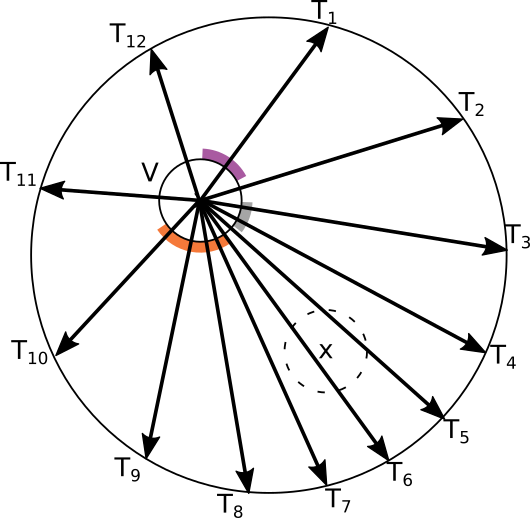
\includegraphics[width=0.9\textwidth]{03/impl_texture_lookup01.png}
            \caption{The rays $T_i-V$ in world space}
    \end{subfigure}%
    \hfill
    \begin{subfigure}[t]{0.3\textwidth}
            \centering
            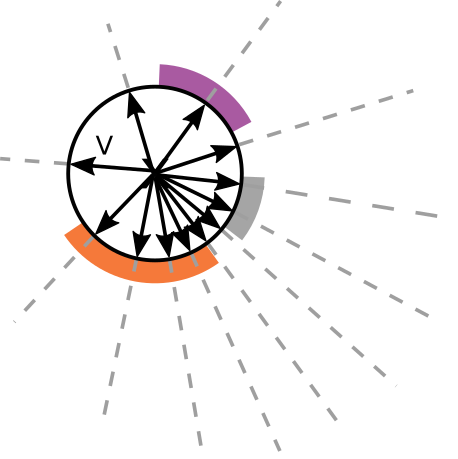
\includegraphics[width=0.9\textwidth]{03/impl_texture_lookup02.png}
            \caption{The normalized rays $T_i-V$ in model space}
    \end{subfigure}
%    \hfill
%    \begin{subfigure}[t]{0.19\textwidth}
%            \centering
%            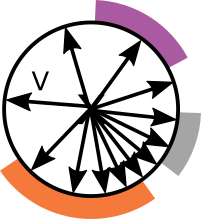
\includegraphics[width=0.9\textwidth]{03/impl_texture_lookup03.png}
%            \caption{}
%    \end{subfigure}%
    \hfill
    \begin{subfigure}[t]{0.3\textwidth}
            \centering
            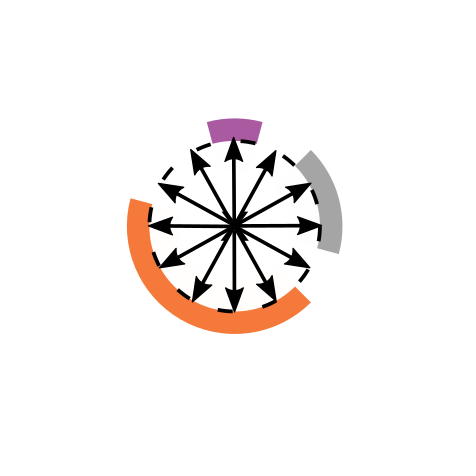
\includegraphics[width=0.9\textwidth]{03/impl_texture_lookup04.png}
            \caption{The result of resampling based on uv coordinates}
    \end{subfigure}%
    \hfill
  \caption{Texture lookup by uv remapping} \label{fig:impl_texture_lookup}
\end{figure}

\subsubsection{Deviation Angle Calculation and Knn Blending}
The deviation angle calculation is a simple angle calculation between vectors. This calculation is performed for each ray of the synthesized point and the corresponding rays of all of the input viewpoints.
Again, the deviation angles per viewpoint are stored in latlong representation (Figure~\ref{fig:dev_angle_storage}a). The deviation angles for all viewpoints are stacked in a three-dimensional matrix, which allows comparison of the deviation angles per pixel/ray of all the viewpoints (Figure~\ref{fig:dev_angle_storage}b). This makes the selection of the best viewpoint per pixel very straightforward, since the id of the k best input viewpoints can easily be extracted and the corresponding pixel value retrieved. With this information, the ``regular'', k-nearest-neighbor (knn) blending is performed.

\begin{figure}
\centering
    \hfill
    \begin{subfigure}[t]{0.4\textwidth}
            \centering
            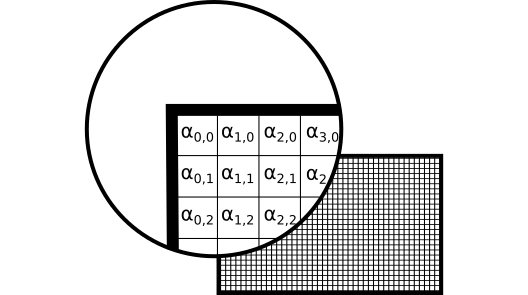
\includegraphics[width=\textwidth]{03/impl_dev_storage01.png}
            \caption{The deviation angles of one input viewpoint in latlong format}
    \end{subfigure}%
    \hfill
    \begin{subfigure}[t]{0.4\textwidth}
            \centering
            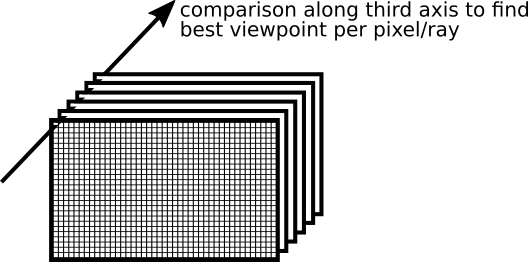
\includegraphics[width=\textwidth]{03/impl_dev_storage02.png}
            \caption{The stacked deviation angles of all input viewpoints}
    \end{subfigure}
    \hfill
  \caption{Visualization of deviation angle storage} \label{fig:dev_angle_storage}
\end{figure}

The regular blending function combines the values of the rays of the k closest deviation angles $\alpha$. The idea behind it is to weight deviation angles of 0 very highly and all larger deviation angles with exponentially low values. This is done with an inverse sigmoid function (Function~\ref{eq:sigmoid}, visualized in Figure~\ref{fig:sigmoid}). The parameters of the function were found by trial and error.

\begin{align}
  w(\alpha) = \frac{1}{(1 + e^{500\cdot(\alpha - 0.017)})} \label{eq:sigmoid}
\end{align}

\begin{figure}
		\centering
		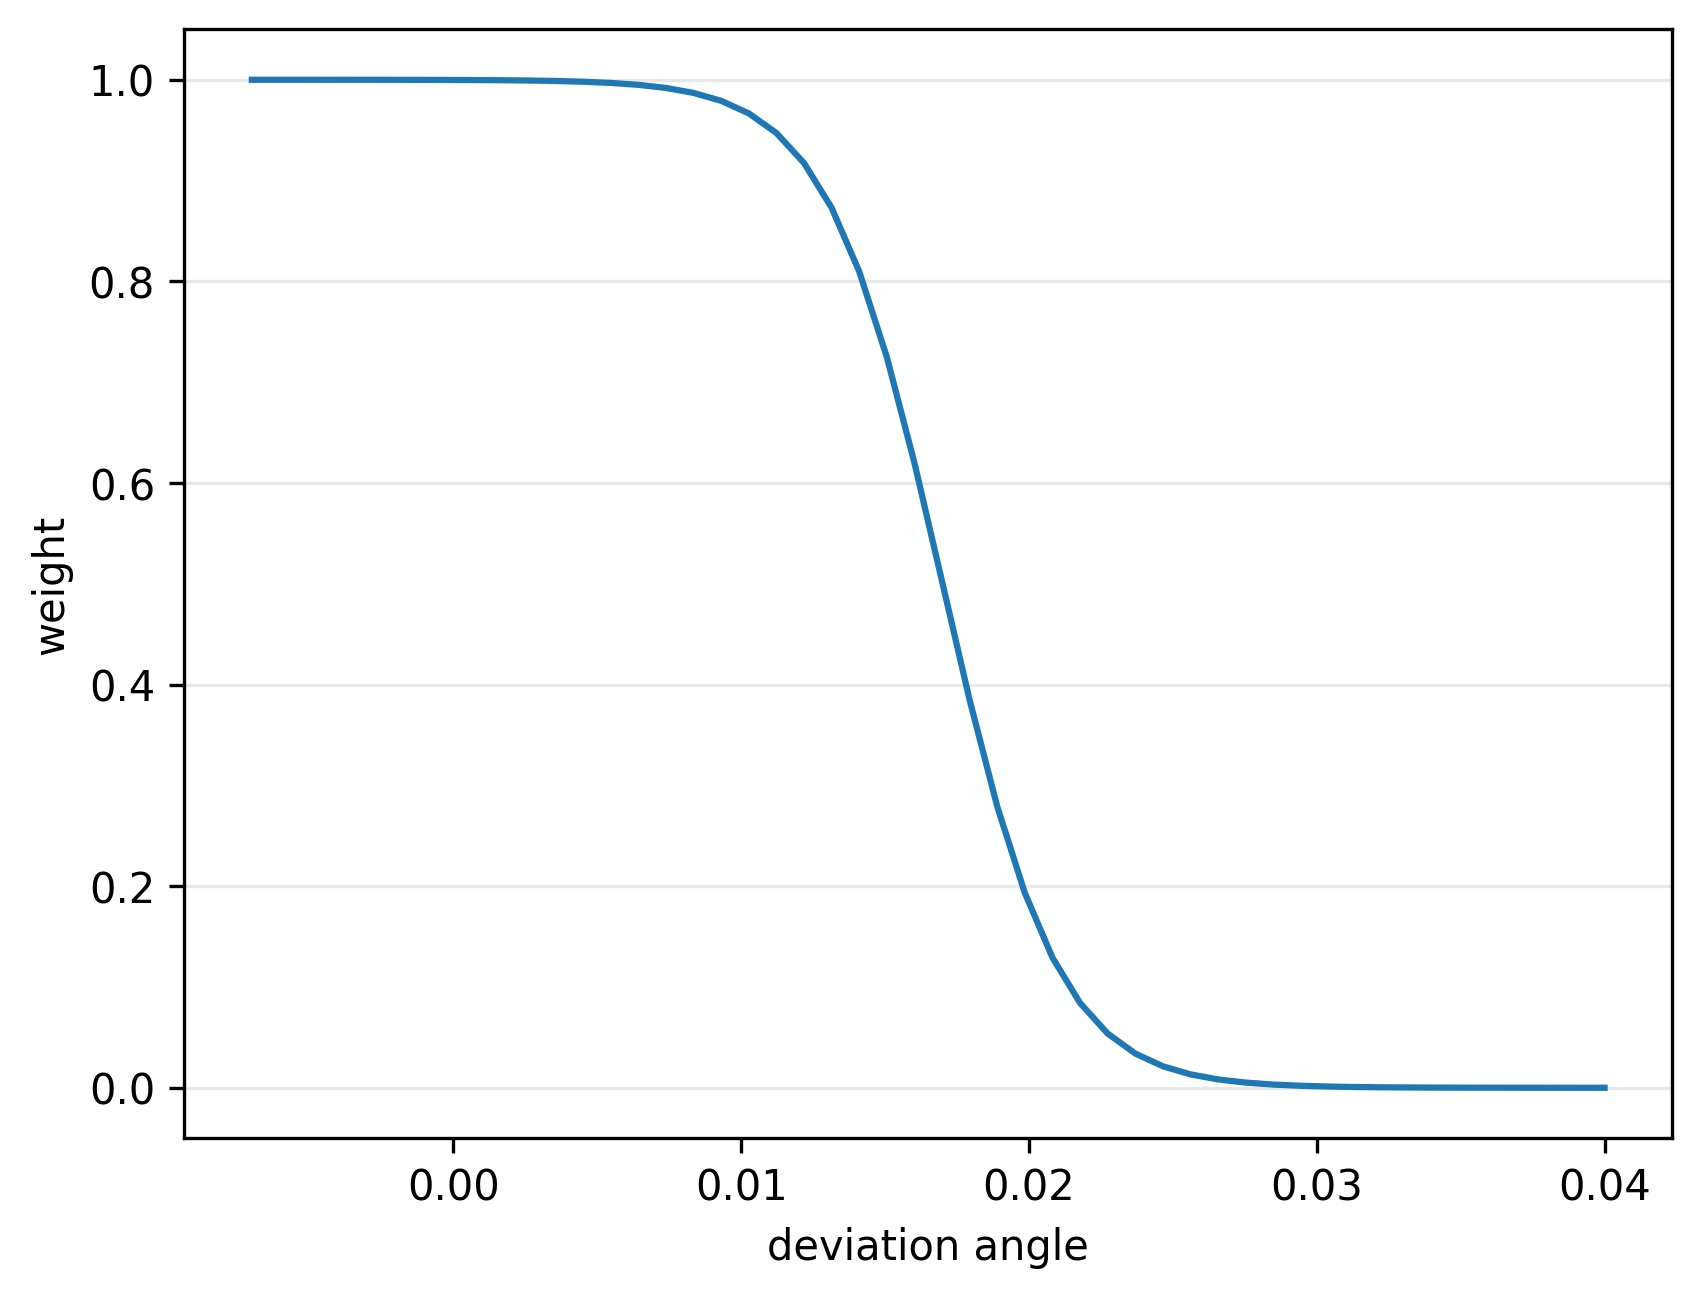
\includegraphics[width=0.5\textwidth]{03/inverse_sigmoid.jpg}
		\caption{The inverse sigmoid function used for weighting}
		\label{fig:sigmoid}
\end{figure}

Then, the per-pixel weights $w$ are normalized so that their sum for each pixel is one, so that the final image is not oversaturated. Finally, the pixel values of the different remapped viewpoints are multiplied by the normalized weights associated with that viewpoint and the weighted latlong images are added up to give the final synthesized image. Blending the two best viewpoints per pixel results in smoother transitions between the mosaicked areas. Figure~\ref{fig:knn} shows the difference between using $k=1$ and $k=2$: It is clearly visible that the border between two mosaicked areas (e.g. on the rug in the center of the room) is very abrupt in Figure~\ref{fig:knn}a, becaulse the two areas do not align perfectly. This border is much smoother in Figure~\ref{fig:knn}b, since the two areas are gradually blended into one another. Using $k>2$ does not have much impact, since most deviation angles where $k>3$ are too large to have an effect.

\begin{figure}
\centering
    \hfill
    \begin{subfigure}[t]{0.5\textwidth}
            \centering
            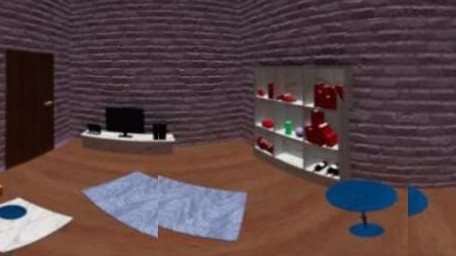
\includegraphics[width=0.9\textwidth]{03/C_max_vps_knn1.jpg}
            \caption{$k=1$}
    \end{subfigure}%
    \hfill
    \begin{subfigure}[t]{0.5\textwidth}
            \centering
            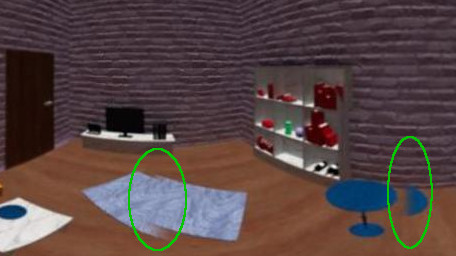
\includegraphics[width=0.9\textwidth]{03/C_max_vps_knn2.jpg}
            \caption{$k=2$}
    \end{subfigure}
    \hfill
  \caption[K-nearest-neighbor blending with different values for k]{K-nearest-neighbor blending with different values for k. The images are clipped from the latlong representation of an image synthesized using regular blending.} \label{fig:knn}
\end{figure}

\subsection{Flow-based Blending}
The 2DoF synthesis with flow-based blending utilizes some steps from the basic 2DoF synthesis, such as the deviation angle calculation and the texture mapping. The details of the input viewpoint selection, the choice of viewpoints A and B for the 1DoF interpolation, the calculation of the interpolation distance $\delta$, as well as the 1DoF intepolation are explained in this section. 

\subsubsection{Selecting Appropriate Input Viewpoints}
The adaptation of optical flow algorithms for 360\degree images, as well as most optical flow algorithms themselves, are limited to a maximumum displacement. This is not considered in the algorithm itself, so it is handled in the input viewpoint selection. The goal of the input selection is to find a minimal convex hull around the point to be synthesized from the set of captured viewpoints. The solution is if there is at least one captured viewpoint in each quadrant around the synthesized viewpoint. If there is no point in one of the quadrants, the points in the quadrants adjacent to the empty quadrant are selected so that they are as close to the empty quadrant as possible. Since the synthesized point is in the convex hull of all the captured points, there must exist a solution for the minimal convex hull. In the worst case, the minimal convex hull is so large that the optical flow algorithm fails.

\subsubsection{Choosing the Viewpoints A and B}
The choice of the input viewpoints A and B for the 1DoF interpolation is important in that two viewpoints need to be chosen that are on either side of the ray in question (see Figure~\ref{fig:flow_vpchoice}), so that the line on which the images can be interpolated actually intersects the approximated ray. Since all the viewpoints are on a plane, the ``side'' a viewpoint is on is defined by whether the deviation angle is between 0 and 180\degree (one side) or between 180 and 360\degree (other side). 
%In order to easily check for the side, a sign is assigned to all deviation angles. Angles $\alpha \in [0,179]$ are assigned a positive sign and angles $\alpha \in [180, 360]$ are subtracted by 360 (to give them the same range) and assigned a negative sign.
To get the best deviation angles on either side, the angles are sorted and the angles closest to 0 and closest to 360 are chosen.

The only problem with this process would arise if there was no viewpoint on the other side of the axis. However, because of the restriction that all synthesized points must be within the convex hull of the captured points, this can never happen. In the worst case scenario, there is only one viewpoint on the other side of the axis with a very large deviation angle. This is acceptable, since this viewpoint is not directly used, instead the 1DoF interpolation creates a new viewpoint with a ideally very small deviation angle.

\subsubsection{Determining the 1DoF Interpolation distance $\delta$}
Given the two viewpoints A and B, it is now possible to calculate the intersection of $\overrightarrow{AB}$ and the approximated ray (elevation $\theta = 0$) between the synthesized point $S$ and the target point $P$ in the scene (Figure~\ref{fig:flow_pos}). The calculation of the intersection between two lines is a simple method based\ldots\todo{either cite or declare as common knowledge} Using these four points A,B,P and S, two infinite lines can be defined (Equation~\ref{eq:lines}). The intersection point at $t * \overrightarrow{AB}$ is given by Equation~\ref{eq:t}.
%Like in basic 2DoF synthesis, having only two input viewpoints A and B trivializes the choice of viewpoints for flow-based blending. For any point in the scene, the ray from the synthesized point is retrieved (same as in basic 2DoF synthesis). However, instead of a texture lookup, the distance factor $\delta \in [0,1]$ of the interpolated viewpoint $vp_{AB}$ is calculated.

\begin{align}
  \overrightarrow{AB} = A + t * (B-A) \quad \overrightarrow{SP} = S + u * (P-S) \label{eq:lines} \\
  t = \frac{(x_A - x_S)(y_S - y_P) - (y_A - y_S)(x_S - x_P)}{(x_A - x_B)(y_S - y_P) - (y_A - y_B)(x_S - x_P)} \label{eq:t}
\end{align}

Since the synthesized viewpoint S is within the convex hull, there is always an intersection t $\in [0,1]$. This value can then directly used as $\delta$. The only case that merits an exception is if the synthesized viewpoint is directly on the border of the convex hull, i.e. directly on the line between two captured viewpoints. In this case, the ray that is parallel to vector $\overrightarrow{AB}$ is equal to the line AB. As a result t is not defined and $\delta$ must be found by dividing the distance $|\overrightarrow{AS}|$ by $|\overrightarrow{AB}|$.

\begin{figure}
\centering
    \hfill
    \begin{subfigure}[t]{0.33\textwidth}            
            \centering
            \includegraphics[width=\textwidth]{03/flow_pos420.jpg}
            \caption{}
    \end{subfigure}%
    \hfill
     %add desired spacing between images, e. g. ~, \quad, \qquad etc.
      %(or a blank line to force the subfigure onto a new line)
    \begin{subfigure}[t]{0.33\textwidth}
            \centering
            \includegraphics[width=\textwidth]{03/flow_pos480.jpg}
            \caption{}
    \end{subfigure}
    \hfill
    \begin{subfigure}[t]{0.33\textwidth}
            \centering
            \includegraphics[width=\textwidth]{03/flow_pos540.jpg}
            \caption{}
    \end{subfigure}
    \hfill
    \caption[Different examples of $\delta$]{Depending on the scene point, a different $\delta$ is calculated based on the intersection of $\overrightarrow{AB}$ and $\overrightarrow{S,target}$} \label{fig:flow_pos}
\end{figure}

\subsubsection{1DoF Interpolation}
Given the two viewpoints A and B and the interpolation distance $\delta$, the interpolated image at $\delta$ between A and B can be calculated. The different steps of the process are extending the cube map, calculating optical flow on the extended cube map, shifting the images by the optical flow, and transforming the shifted, extended cube map back into latlong representation so that it can be remapped used for blending.
\missingfigure{1DoF process diagram}

\paragraph{Extended Cube Map}
The class \emph{ExtendedCubeMap} uses the 360\degree image data and the virtual camera provided by skylibs \cite{skylibs} to ``extend'' the cube map by capturing a virtual image for each face of the cube with a 150\degree field of view. This is done for both viewpoints A and B. The \emph{ExtendedCubeMap} class handles the extended faces and can perform different functions on them, for example the optical flow calculation, which is required for the next step.

\paragraph{Optical Flow Calculation and Image Shifting}
The optical flow algorithm used in the implementation is Farneb\"ack's algorithm implemented by OpenCV (\emph{cv2.calcOpticalFlowFarneback}) \cite{opencv}. For calculating optical flow between two \emph{ExtendedCubeMaps} A and B, the \emph{ExtendedCubeMap} class provides a function \emph{optical\_flow}, which takes as arguments the optical flow algorithm, and a second \emph{ExtendedCubeMap} to use for optical flow calculation. Passing the optical flow function dynamically greatly simplifies exchanging the optical flow algorithm for future work.

The \emph{ExtendedCubeMap} then calculates the optical flow \emph{separately} between each corresponding pair of extended faces. On top of the optical flow from \emph{ExtendedCubeMaps} A to B, the inverse optical flow from \emph{ExtendedCubeMaps} B to A is required as well. The inversion of optical flow is nontrivial\todo{maybe illustrate}, since inverting the optical flow vectors is not enough: The vectors must be shifted by their identity and then reversed. Alternatively, the optical flow can just be calculated on the \emph{ExtendedCubeMaps} in reverse, i.e.\ from B to A. This option is used in the proof-of-concept implementation in order to avoid bugs, and since the impact on performance is not very high for images with small resolution, which are used in Chapter~\ref{chap:evaluation}.

Using the optical flow, the inverted optical flow, and the interpolation distance $\delta$, the shifted images $I_A$ and $I_B$ are calculated seperately for each face by again using Scipy's \emph{scipy.ndimage.map\_coordinates}, with image coordinates shifted by the optical flow vectors and $\delta$, and the inverse optical flow vectors and $(1-\delta)$, respectively. The shifted \emph{ExtendedCubeMap} images are then combined by multiplying them by $(1-\delta)$ and $\delta$, respectively, and adding the pixel values. The result is an interpolated \emph{ExtendedCubeMap} at interpolation distance $\delta$.

Before passing this on to the blending step of the 2DoF synthesis, the \emph{ExtendedCubeMap} is transformed back into a regular cube map by clipping each face back to its original size and mapping the cube map back to a latlong map, since all other processing steps use the latlong format.

\subsubsection{Flow-based Blending}
The flow-based blending step combines all of the previous steps: first, for each ray, the viewpoints A and B are selected and the interpolation distance $\delta$ is calculated. Then, a mask is created for each set $(A,B,\delta)$, masking all pixels that do not belong to the set, and the interpolated image for that set is calculated. This is repeated for all sets.

The complexity of the flow-based blending is directly bound to the precision of $\delta$. Given a precision of two decimal points results in 101 different interpolated images ($\delta \in [$0.00, 0.01, 0.02 \ldots 0.99, 1.00$]$), whereas precision of one decimal point results in only 11 calculated images. A precision of two is used in the implementation, since this is an acceptable compromise between complexity and a result with smoother transitions.

Finally, the masked interpolated latlong images are added together to give the final result.

\subsection{Performance}
As this is a first attempt at 2DoF synthesis, performance was not deemed important, and no parallelizations were incorporated. Since the algorithms operates pixel-wise, the computation time increases exponentially for larger image resolutions ($O(n^2)$ coplexity). The performance of the flow-based blending depends on the location of the synthesized point in relation to the captured points. In the worst case, one interpolated image must be calculated per pixel, at best one interpolated image must be calculated for the whole image (if a synthesized viewpoint is directly on a line between two captured viewpoints). The non-optimized interpolation of a whole image for pixel regions (and in the worst case, single pixels), makes the flow-based blending significantly slower than the regular blending.

The synthesis of an image of 1000x500 pixels with no optimization using regular blending with 4 input viewpoints takes approximately 4s on a single Intel Xeon (Skylake) processor, whereas flow-based blending with the same input takes between 10 and 30 minutes, depending on the constellation of the viewpoints.
Fortunately, many of the operations are ``embarrassingly parallel'', meaning they can be very easily parallelized, which will be discussed in Section~\ref{sec:future_work}.

\subsection{Implementation-related Problems}
Unfortunately, there are some implementation-related problems that are unrelated to the algorithm, but nonetheless have an effect on the result. The extension of the regular cube map to the \emph{ExtendedCubeMap} with the skylibs library slightly distorts the image for an as-of-yet unknown reason, so that when the map is clipped back down to its regular size, it is not identical to the original. Although the difference not extreme, it is nonetheless noticeable.

The other, more visible problem, also from the skylibs library, concerns the conversion from the cubemap back to the latlong representation. Due to a bug in this operation, a black line sometimes appears at on or more borders of a face. Since the synthesized images are made up of mosaicked, reprojected areas, it is possible that in some cases, these lines shift into the middle of faces.

Both of these errors are relatively small, and their effect is negligible compared to some of the algorithm-related artefacts, so they can be disregarded.

    \chapter{Evaluation and Results} \label{chap:evaluation}
%One liability of image-based rendering systems is the lack of a consistent  framework within which to judge the validity of the results. plenoptic modeling: an image-based rendering system mcmillan
Unfortunately, there are no publicly available benchmarks for 360\degree image synthesis with two degrees of freedom without 3D geometry, as not many methods exist that try to achieve this. Since the approach presented in Chapter~\ref{chap:implementation} is a first, basic attempt at solving this problem, this chapter presents a basic evaluation of the algorithm, based on mathematically calculable error metrics. These metrics measure the accuracy of a synthesized image compared to the ground truth and are used to assess the effect of a limited number of parameters.
%Furthermore, it compares the results of regular blending, flow-based blending, and a na\"ive baseline algorithm to analyze whether, and in which cases an improvement could be achieved.

First, possible parameters are discussed (Section~\ref{sec:params}), followed by the presentation of the evaluation methodology (Section~\ref{sec:eval_methodology}). Then a detailed evaluation is performed on virtually generated scenes to explore the limits of the algorithm in a controlled environment (Section~\ref{sec:limit_eval}). Based on the knowledge gained in the limit evaluation, a proof-of-concept evaluation is performed on real scenes (Section~\ref{sec:pof_eval}). Finally, the limitations of the evaluation and algorithm are discussed (Section~\ref{sec:limitations}).

%First the evaluation methodology is presented, outlining how the effects of a parameter are measured and evaluated. Then, the limits of the algorithm are explored using virtual scenes. With the information gleaned from this limit evaluation, the parameters are chosen for a proof-of-concept evaluation using real scenes. The results and limitations are then discussed\ldots

%- what is a scenario what is a scene
%- not performance
%- konkreter
%- wie gut koennen szenen synthetisiert werden
%- scope: basic evaluation of mathematically measurable values (no human perception)
%- these datasets could be used in the future to compare different algorithms

\section{Parameters} \label{sec:params}
Before defining the parameters to test in the limitation and proof-of-concept evaluations, this section gives an overview of possible parameters in the context of the 2~DoF algorithm presented in Chapter~\ref{chap:implementation}.
The 2~DoF algorithm already makes a few assumptions, for example the constraint to the viewpoint plane, the fact that the scene is static, and more (stated in Section \ref{sec:approach} on page \pageref{sec:approach}). These assumptions are upheld in the evaluation, as they are prerequisite to the function of the algorithm.
\todo{define performance as accuracy of results based on error metrics}

The remaining parameters (that are not constrained by the assumptions) can be divided into two categories: 
\begin{description}
    \item [Internal parameters] i.e.\ based within the algorithm, such as the blending type and the selection of input viewpoints
    \item [External parameters] i.e.\ based on the properties of the captured scene, such as the viewpoint density, or the geometry of the scene.
\end{description}      

The internal parameters can be modified after the scene has been captured, the external ones cannot.  The most prominent internal parameters based on the implementation from Chapter~\ref{chap:implementation} are:

\begin{itemize}
  \item the location of synthesized points within the scene (near walls, objects, etc)
  \item the location of synthesized points relative to the captured points
  \item the blending type, i.e.\ flow-based blending or deviation-angle-based knn blending (``regular blending'')
%  \item the selection of input viewpoints from the available captured viewpoints
  \item the optical flow algorithm used for flow-based blending
\end{itemize}

There are more internal parameters that could theoretically be modified, such as the knn blending function (the inverse sigmoid function on page~\pageref{eq:sigmoid}), or the method of approximation for 2~DoF in flow-based blending (page~\pageref{subsec:2dof_flow-based}), but these will be assumed immutable for this evaluation, as the variation of these parameters would require developing new functions, which would be outside the scope of this thesis.

As for the possible external parameters, the number of different possible scenes is infinite, but the assumed key parameters are:
\begin{itemize}
  \item type of scene (outdoor, indoor, etc) \ar size and shape of scene
  \item objects within the scene
  \item density of captured viewpoints
  \item distribution of captured viewpoints
\end{itemize}

External parameters such as the camera settings (e.g. aperture, shutter speed, white balance) and the lighting throughout the scene are not considered; it is assumed that all the captures have the same camera settings and the white balance is comparable throughout the scene. Furthermore, the evaluation is restricted to indoor scenes of approximately $25m^2$. This reduces the parameter space significantly, since the fact that indoor scenes tend to be enclosed by walls enforces a maximal distance of objects to the camera.

The evaluation presented in this thesis aims to examine the effects of a few select internal and external parameters, instead of exhaustively examining all of them. In order to do this, a \emph{scenario} is designed for each selected parameter that attempts to demonstrate the effect of this parameter on the accuracy of the result. Limiting the evaluation to specific scenarios reduces the testing space but might also lead to missing some interactions between parameters. This is acceptable, since the evaluation does not aim to be comprehensive. 

%The scenario definition is the first step of the evaluation process which is presented in the next section.
%The parameters to be evaluated, along with their corresponding scenarios depend on the type of evaluation

\section{Evaluation Methodology} \label{sec:eval_methodology}
The evaluation is divided into two distinct phases: an evaluation of limits using virtual scenes, and a proof-of-concept evaluation using real scenes. Both evaluations follow the methodology depicted in Figure~\ref{fig:eval-methodology}, and consist of four steps: \emph{scenario definition}, where a scenario is designed to exemplify the parameter to test, \emph{synthesis}, where the synthesized images are calculated using the 2~DoF synthesis presented in Chapter~\ref{chap:implementation}, \emph{error calculation}, where the accuracy of the synthesized images is measured, and \emph{result analysis}, where the the cause and effect of the parameters is examined. The details of these steps are described in the following sections.

\begin{figure}
		\centering
		\includegraphics[width=\textwidth]{04/eval_methodology.png}
		\caption{Methodology for the evaluation of a scenario}
		\label{fig:eval-methodology}
\end{figure}

\subsubsection{Scenario Definition}
A scenario is defined by the parameter that it tests, the static parameters that are used, and the scene where the data was captured. Although a scenario is designed to test a specific parameter, which then is ``dynamic'' (i.e.\ will be modified throughout the scenario), there might also be more dynamic parameters. For example, in a scenario for exploring viewpoint density, the blending type might also be modified to see what effect the viewpoint density has on regular and flow-based blending. The static parameters include for example the location of the synthesized viewpoints, or any other parameter that remains unchanged throughout the scenario. One other defining factor of a scenario is the scene data that the scenario is tested on. Although the scene is part of the parameters (the external parameters, to be exact), it merits particular mention, as it contains the actual image data that is used for synthesis. This data, along with the other parameters defined in the scenario, are then passed on to the synthesis step.

%First, a scenario must be defined that illustrates the parameter that should be examined. This includes determining which of the parameters should be static, and which should be dynamic. There are two dynamic parameters at maximum, one to be examined, and one to increase the significance of the results. Adding more dynamic parameters per scenario would allow for a more definitive evaluation, but is outside of the scope of this thesis.

%The set of parameters (whether static or dynamic) contains the choice of scene in which to synthesize the images. The scene is defined by its captured viewpoints, metadata, and radius, which are all passed on to the synthesis step along with the other parameters defined for the scenario.

\subsubsection{Synthesis}
The synthesis step consists of two parts: the 2~DoF synthesis presented in Chapter~\ref{chap:implementation} using either flow-based blending or regular blending depending on the scenario parameters, and a baseline synthesis using a na\"ive algorithm.
The na\"ive algorithm consists of simply selecting the nearest neighbor viewpoint based on euclidean distance. The input parameters are the same for both algorithms and both results are passed on to error calculation.
The results of the na\"ive algorithm serve as a baseline comparison to verify whether the developed 2~DoF algorithm is an improvement to a na\"ive approach. If either the regular or the flow-based blending generally performed worse than the na\"ive algorithm, this would be an indication of a substantial flaw in the approach.
\todo{use naive algo or not?}

\subsubsection{Error Calculation}
There are many properties that a synthesis algorithm can be evaluated for, for example performance, visual acceptability (based on user studies), number of artefacts, or distance from the ground truth. In this evaluation, mathematical
%In order to evaluate the synthesized images, it is necessary to define metrics with which to measure their accuracy. Since it is outside of the scope of this thesis to evaluate the quality of the results based on human perception, mathematical
error metrics are used to compare each result to its ground truth image.  Two different metrics are chosen based on different image features so that potential limitations of each metric can be compensated for by the other. However, it must be taken into account that neither are perfect for the task of measuring accuracy on 360\degree synthesized images, so their validity should always be taken with a grain of salt. 

\paragraph{L1 error on RGB}
The first metric is the L1 error calculated on the ground truth and result images in RGB color space. This is a simple error metric that calculates the mean absolute difference of the RGB values and therefore indicates the mean accuracy of each pixel of the image. The RGB errors of each pixel are added together for the complete image and then divided by the number of pixels in the image. This results in an error value $e \in [0,3]$, since the maximum error per pixel is 3 for floating point RGB color values $\in [0,1]$.

The L1 error can also be visualized by calculating the absolute difference per pixel without averaging the values. Figure~\ref{fig:l1_example} shows an example visualization of the L1 error between two images. The visualization encodes areas of the image where there is a very large difference with a value closer to white and areas where there is no difference as black, which clearly highlights areas of the image that are problematic.

The L1 error is useful because it gives a rough estimation of how accurately each pixel is synthesized. The visualization indicates in which areas the synthesized image is inaccurate, which is helpful for classifying problems. However, a drawback of the L1 error is that it relies on color values, which means that images with large differences in pixel values will generally produce a higher error value than images with smaller differences in pixel values, even though the distortion and displacement may be the same.

\begin{figure}
\centering
    \hfill
    \begin{subfigure}[t]{0.3\textwidth}
            \centering
            \includegraphics[width=0.9\textwidth]{04/l1_ex01.jpg}
            \caption{}
    \end{subfigure}%
    \hfill
    \begin{subfigure}[t]{0.3\textwidth}
            \centering
            \includegraphics[width=0.9\textwidth]{04/l1_ex02.jpg}
            \caption{}
    \end{subfigure}
    \hfill
    \begin{subfigure}[t]{0.3\textwidth}
            \centering
            \includegraphics[width=0.9\textwidth]{04/l1_ex03.jpg}
            \caption{L1 error visualization of (a) and (b)}
    \end{subfigure}%
    \hfill
    \hfill
  \caption[Example visualization of L1 RGB error]{Example visualization of L1 RGB error. The RGB error values have been intensified so that they are more visible.} \label{fig:l1_example}
\end{figure}

As in the case of optical flow calculation, some adjustment must be made to adapt this metric for 360\degree images. Since the equirectangular projection is not equal-area, the areas towards the poles would intrinsically have higher weighting, since RGB L1 is calculated per pixel. To avoid this problem, the cube map projection is used, since it does not significantly distort the image. The average value is then calculated using the six faces of the cube, omitting the black background.

\paragraph{SSIM error on Grayscale}
The metric to complement the RGB L1 error is a variation of the the structural similarity index (SSIM) \cite{ssim}, which measures the \emph{structural similarity} between two images. Instead of comparing the images pixel by pixel, the SSIM uses the luminance, contrast and structure of the images for comparison. It compares these locally, i.e.\ it operates on smaller areas instead of the image as a whole. As a result, it is possible that the SSIM does not register small displacements in the scene if the objects are not distorted. However, the additional comparison with the RGB L1 error should mitigate this potential problem.

The SSIM metric in general, and the implementation used in the evaluation\footnote{skimage.metrics.structural\_similarity \cite{skimage}} return a value $\in [-1, 1]$ with 1 signifying an extremely similar image and -1 signifying a very different image. In order to more easily compare it with the RGB L1 error, the SSIM value is converted to an error value $ e \in [0,1]$, with 0 signifying an identical image (0 error) and 1 signifying a very different image.

The SSIM error is calculated on the grayscale image in cubemap representation. There is no need to use an RGB image, since it does not use the color values of an image. To avoid possible problems with distortion, the cubemap representation is again used.

\subsubsection{Result Analysis}
For each scenario evaluation, the number of results is made up of the dynamic parameters, the number of synthesized viewpoints, plus the baseline results. For each image, there are two error metrics to be considered.
%The number of parameters combined with the comparison to the baseline results and the use of two different error metrics results in a large number of error values.
In order to analyze these results effectively, it is necessary to break them down by creating different visualizations that highlight different attributes of the results.At first, an overview is created, from which interesting cases are selected and examined in more detail.

\paragraph{Distribution Comparison}
The first step of the analysis is a comparison of error value distribution. In order to compare all the error values of a scenario, they are plotted using a boxplot (Figure~\ref{fig:boxplot_example}). The different parameter combinations of the scenario are plotted on the y axis (e.g. viewpoint densities a, b, c) and the error distribution (i.e.\ the error values of all the synthesized viewpoints) is plotted on the x axis. The box plot shows the distribution of these values: the thick black line in the colored box is the median value (approx. 0.184 in Figure~\ref{fig:boxplot_example}), the colored ranges to the left and right of the median describe the ``interquartile range'' (IQR), the range of the closest half of the data (25\% on each side). The ``whiskers'' of the plot extend to the minimum and maximum of the values. The minimum and maximum are defined as $1.5\cdot IQR$. Any data outside of the the range between the minimum and the maximum, are the ``outliers'', depicted as small crosses. The boxplot gives a general overview of how the error values of the specific scene are distrubute. The distribution of the error values of the results in Figure~\ref{fig:boxplot_example}, for example, shows that the first three quartiles of the results are fairly close to the median (between approx. 0.14 and 0.19), whereas the fourth quartile extends, over almost the same range (0.19 to 0.225) and there are some extreme outliers. This indicates that there are some viewpoints that performed significantly worse than most of the others.

\paragraph{Scene Analysis}
Based on the insights gained in the distribution comparison, several interesting cases are selected for closer analysis. These cases are examined by color coding the error values and assigning the colors to the positions in the scene. This puts the error values in context with the scene surroundings. Figure~\ref{fig:posmap_example} shows the synthesized points in the context of the scene, color coded by their error values. The maximum and minimum values of the points (also clearly visible in Figure~\ref{fig:boxplot_example}) are coded as light green and dark blue, respectively. This visualization gives a more detailed overview over the values of the different points. In Figure~\ref{fig:posmap_example}, for example, the synthesized points near the right wall of the room have much better values than the row on the left side of the room. The four light green values are clearly the outliers that were visible in Figure~\ref{fig:boxplot_example}. Using this information, it is possible to draw som conclusions about the effect of the position of the synthesized viewpoint relative to the objects in the scene, and select a few synthesized images that merit closer examination.

\begin{figure}
\centering
    \hfill
    \begin{subfigure}[c]{0.5\textwidth}
            \centering
            \includegraphics[height=6cm]{04/boxplot_example.jpg}
            \caption{Boxplot example for distribution comparison of the results of regular blending in the ``square room''} \label{fig:boxplot_example}
    \end{subfigure}%
    \hfill
    \begin{subfigure}[c]{0.5\textwidth}
            \centering
            \includegraphics[height=6cm]{04/posmap_example.png}
            \caption{Visualization for scene analysis: The error values from the boxplot in (a) are mapped to colors at the positions of the viewpoints in the scene. Light green represents the worst value (approx. 0.27) and dark blue the best value (approx. 0.145).} \label{fig:posmap_example}
    \end{subfigure}
    \hfill
  \caption[Different types of result visualizations for L1 error values]{Different types of result visualizations for L1 error values (``rgb\_l1'') for example results of regular blending in a scene}
\end{figure}
\todo{replace figures (colors and error metric names}

\paragraph{Sample Inspection}
In order to further understand the effects of the parameters on specific positions, some of the synthesized viewpoints from the scene analysis are examined manually by comparing the synthesized image to the ground truth image. The visual examination may also reveal information that the error metrics are unable to extract, such as specific types of artefacts. For example, by using the information presented in Figure~\ref{fig:posmap_example}, it is possible to choose one of the best results, for example synthesized point ``K'' near the right wall in the middle. The close inspection of the synthesized images is shown in Figure~\ref{fig:inspection_example} (page~\pageref{fig:inspection_example} in Appendix~\ref{imgs}\footnotemark): In the left column from top to bottom are the ground truth image, the synthesized image using regular blending, and the synthesized image using flow-based blending. In the right column are the L1 difference images to the ground truth image. They can help with understanding the error values. For example, the rug in the bottom face (green ring) is improved in the flow result compared to the regular result in Figure~\ref{fig:inspection_example}. However, the flow result also has a fairly large artefact at the top of the door in the left face (magenta ring), which is not the case in the regular result. The green rings show improvements, and the magenta rings show artefacts or other problems.\todo{color coding of marks?}
\footnotetext{The synthesized images are shown in Appendix~\ref{imgs}, in order to avoid interrupting the flow of the text, since they take up a fairly large amount of space.}















\section{Evaluation using Virtual Scenes} \label{sec:limit_eval}
In the first part of the evaluation, virtual scenes are used to evaluate the effect of a chosen set of internal and external parameters on the accuracy of the results of the 2~DoF synthesis.
Virtual scenes allow full control over the external parameters, for example the scene geometry, and the positions of the captured viewpoints, as well as being less error prone than manual capture, where positional and rotational inaccuracies may be introduced. This also 
\todo{eek}
As a result, virtual scenes make it possible to test setups that would be unfeasible for real scenes, for example using a large number of captured viewpoints at varying locations in different scenes.
Additionally, since the evaluation is based on comparing the synthesized images to the ground truth, it is necessary to capture the ground truth images, along with the input viewpoints.
As a result, the scenarios can be designed independent of the constraints of the manual capture of real scenes.
%this limit evaluation is performed on virtual scenes created with the open source 3D animation software Blender \cite{blender}.
%The first step of the evaluation is to test the parameters of choice in a way that explores a large range of \ldots cases. 
The parameters that will be explored in the scenarios are:
\begin{itemize}
  \item proxy-scene difference (how dissimilar is the scene geometry from the proxy sphere geometry, including the objects within the scene)
  \item density of the captured viewpoints
  \item position of the synthesized points relative to the captured points
%  \item flow-based blending compared to regular blending
\end{itemize}

A scenario is designed for each of the three parameters, containing several different setups that are meant to test the limitations of the algorithm developed in Section~\ref{chap:implementation}. 

%Another factor that will be considered in all of the scenarios is the impact of the proximity and complexity of objects within the scene. However, since this is hard to parametrize, it will not be measured or explicitly tested.

%There is one internal parameter that is not specifically tested, but needs to be addressed, since it has a significant effect on the outcome of the flow-based blending: the optical flow algorithm. Fortunately, using virtual scenes generated with Blender can help mitigate mitigate this problem, since Blender has the capabilities to retrieve movement vectors from the geometry data, which can be used as optical flow.

\subsection{Data Acquisition and Featured Scenes} \label{subsec:data_acquisition}
%In order to be able to test these scenarios, it is necessary to generate appropriate scenes. However, the manual capture of viewpoints as well as ground truth data can be very time-consuming. Furthermore, since locations need to be recorded either by hand, or calculated by a structure-from-motion algorithm or something similar, it is possible that the final locations are not perfectly accurate. In order to circumvent these problems, virtual scenes are used for the evaluation of limits. 


Three different scenes were modeled for testing, using the animation software Blender \cite{blender}: the \emph{checkersphere}, the \emph{square room} and the \emph{oblong room}.% and the \emph{oblong room II}.

\paragraph{Checkersphere}
The \emph{checkersphere} (Figure~\ref{fig:checkersphere}) is a perfect sphere with a diameter of approximately 2m. Its surface is covered with a checkerboard pattern with alternating colors of dark blue, dark red, and dark green. It represents a scene where the geometry of the scene is exactly the same as the proxy geometry. Although this kind of room is not likely to exist in reality, it serves as a good baseline, since the result of the reprojection should be very close to the ground truth. The checkerboard pattern was chosen so that distortions or inaccuracies are more visible.


\paragraph{Square Room}
The \emph{square room} (Figure~\ref{fig:square_room}) is a room whose basic shape is a perfect cube with a side length of 3.5m. It contains an assortment of furniture\footnotemark: In one corner, there is an orange, L-shaped couch with dark blue and white cushions and a white marble coffee table with a dark blue bowl on it, and several small, simple black and white pictures on the wall behind the couch. There is a blue and white rug in the middle of the room, and to the left of the couch are a round blue table, as well as a white radiator. On the wall next to the blue table is a white marble bookshelf containing several red books, as well as three wine bottles, and two decorational objects in green and purple. Across from the couch is a low marble cabinet with a black monitor, a black laptop and a black speaker on it. To the left of the cabinet is a wooden door with a gray handle. The walls are brick, painted a dark purple and there is a lamp with a white lampshade hanging from the middle of the ceiling.

\footnotetext{The furniture models used in the square room and the oblong room are adapted from \url{https://www.cgtrader.com/free-3d-models/interior/living-room/low-poly-interior-57731178-c955-4625-9e44-109c8eea5ee2}, by user ``miha29076'', and the textures are adapted from \url{https://www.poliigon.com/texture/plaster-17}, \url{ https://www.poliigon.com/texture/fabric-denim-003}, \url{https://www.poliigon.com/texture/wood-fine-dark-004}, and \url{https://www.poliigon.com/texture/interior-design-rug-starry-night-001}. \emph{All accessed last on September 23, 2020}}

The intention of using the square room is to allow approximate accuracy for the reprojection step, while at the same time offering a more realistic indoor setting.

\paragraph{Oblong room}
The \emph{oblong room} (Figure~\ref{fig:oblong_room}) has a room size of approximately 5.5m x 3.5m and contains the same basic elements as the square room. It has the exact same furniture layout as the square room, except that some objects 

%The \emph{oblong room} (Figure~\ref{fig:oblong_room}) has a room size of approximately 5.5m x 3.5m and contains the same basic elements as the square room. There are two variations: the oblong room I, which has the exact same furniture layout as the square room, and the oblong room II, in which the furniture layout is modified. This modification can help in examining possible correlations of the scene geometry with the result. For example, the bookshelf is a fairly complex geometry that is at eye-level (as opposed to many other objects which are below eye-level). Placing it at different positions in the two scenes makes the correlation between the proximity to the bookshelf and the possibly worse results easier to recognize.

\begin{figure}[p]
\centering
    \hfill
    \begin{subfigure}[t]{0.7\textwidth}
            \centering
            \includegraphics[height=5cm]{04/checkersphere_overview.jpg}
            \caption{Latlong image from the center of the sphere}
    \end{subfigure}%
    \hfill
    \begin{subfigure}[t]{0.3\textwidth}
            \centering
            \includegraphics[height=5cm]{04/checkersphere_outside.jpg}
            \caption{View from the outside for reference}
    \end{subfigure}
    \hfill
  \caption{Overview of the ``checkersphere''}
  \label{fig:checkersphere}
\end{figure}

\begin{figure}[p]
\centering
    \hfill
    \begin{subfigure}[b]{0.7\textwidth}
            \centering
            \includegraphics[height=5cm]{04/square_overview.jpg}
            \caption{Latlong image from the center of the room}
    \end{subfigure}%
    \hfill
    \begin{subfigure}[b]{0.3\textwidth}
            \centering
            \includegraphics[height=5cm]{04/square_top.jpg}
            \caption{Top view}
    \end{subfigure}
    \hfill
  \caption{Overview of the ``square room''}
  \label{fig:square_room}
\end{figure}

\begin{figure}[p]
\centering
    \hfill
    \begin{subfigure}[b]{0.7\textwidth}
            \centering
            \includegraphics[height=5cm]{04/oblong_overview.jpg}
            \caption{Latlong image from the center of the room}
    \end{subfigure}%
    \hfill
    \begin{subfigure}[b]{0.3\textwidth}
            \centering
            \includegraphics[width=5cm]{04/oblong_top.jpg}
            \caption{Top view}
    \end{subfigure}
    \hfill
  \caption{Overview of the ``oblong room''}
  \label{fig:oblong_room}
\end{figure}

\begin{figure}
\centering
    \hfill
    \begin{subfigure}[b]{0.4\textwidth}
            \centering
            \includegraphics[width=0.9\textwidth]{04/vps_checkersphere.jpg}
            \caption{The captured viewpoints in the checkersphere}
    \end{subfigure}
    \hfill
    \begin{subfigure}[b]{0.4\textwidth}
            \centering
            \includegraphics[width=0.9\textwidth]{04/vps_square.jpg}
            \caption{The captured viewpoints in the square room}
    \end{subfigure}
    \hfill
    \hfill

    \hfill
    \begin{subfigure}[b]{0.4\textwidth}
            \centering
            \includegraphics[width=0.9\textwidth]{04/vps_oblong.jpg}
            \caption{The captured viewpoints in the oblong room}
    \end{subfigure}
    \hfill
    \hfill
  \caption[The grid of captured viewpoints in each scene, including the proxy geometry]{The grid of captured viewpoints in each scene, including the proxy geometry (not to scale)} \label{fig:vps_grid}
\end{figure}

\paragraph{}
Given the different scenes, it is necessary to choose comparable viewpoints to capture that will be used as input for the synthesis. Since the scenes all have similar scale, the viewpoint layout was chosen to be identical in all of the scenes. This means that all scenes contain 36 captured viewpoints, aligned in a regular grid of 6x6 viewpoints, with 60cm spacing. The grid of viewpoints is centered within the scene. This means that in the checkersphere (Figure~\ref{fig:vps_grid}a) and the square room (Figure~\ref{fig:vps_grid}b), the viewpoints cover approximately the complete scene, and in the oblong room, there is about a 1m area on each side of the grid that is not captured (Figure~\ref{fig:vps_grid}c and Figure~\ref{fig:vps_grid}d). It is necessary to take this difference in viewpoint coverage into account for the evaluation, since the viewpoints in the oblong room have a larger distance to two of the walls, which may have an effect on the accuracy of the results.

Since Blender is designed for creating animated movies, and not the capture of static viewpoints, some adjustments had to be made to be able to capture the chosen viewpoints (as well as the ground truth images): After choosing the positions of the input viewpoints for the scenes, the position of the camera for each captured viewpoint was stored as a keyframe, so that the batch of viewpoints could be rendered like an animation. In order to automatically assign the viewpoints and the ground truth points to the keyframes, and write out the metadata, a blender script was implemented. This way the locations of the viewpoints would always be perfectly accurate, and the ``capture'' of the viewpoints required no manual effort. The images were rendered with a resolution of 1000x500 for all of the scenes, in order to reduce the computation time for the image synthesis in the tests.


%, and the same number of synthesized viewpoints (25). Figure~\ref{fig:scene_setup} show how the points are set up in the different scenes. Using the same distances between viewpoints is important for comparing the accuracy (since larger distances may have an impact on the optical flow result), so the space occupied by the viewpoints is proportionally smaller in the oblong rooms (i.e. the viewpoints are not distributed in the entire room). This must be considered when evaluating the results.

\subsection{Synthesizing Ground Truth Optical Flow} \label{subsec:gt_of}
Using Blender to create virtual scenes not only facilitates capture, but also offers an alternative to calculating optical flow. As mentioned in Section~\ref{subsec:optical_flow}, most optical flow algorithms struggle with large displacements. The flow-based blending step in the 2~DoF synthesis algorithm, on the other hand, assumes decent optical flow and there is no attempt to judge whether the optical flow calculation is feasible between two selected viewpoints. As a result, given the wrong circumstances (two viewpoints A and B that are far apart), the optical flow algorithm may fail, leading the flow-based blending to output undesirable results. The success of the optical flow algorithm is a prerequisite for the success of the 2~DoF algorithm with flow-based blending.

However, the focus of this evaluation is not the accuracy of an arbitrary optical flow algorithm. In the best case, it would be possible to emulate ``perfect'' optical flow, thus decoupling the success of the optical flow from the success of the flow-based blending. While this is practically impossible for real scenes, virtual scenes theoretically contain all necessary information for retrieving ``ground truth'' optical flow. Blender, for example, is capable of ``rendering'' motion vectors using its vector speed render pass, which calculates the movement between points from one frame to the next in pixel space. The result is a motion vector field, which corresponds to the result of a ``classic'' optical flow algorithm. This, in the best case, ``ground truth'' optical flow was first presented by Butler et al.\ \cite{sintel} as a benchmark for optical flow algorithms.

In order to demonstrate the improvement of Blender optical flow compared to Farneb\"ack optical flow, which is the optical flow algorithm used in the implementation, Figure~\ref{fig:of_comparison}a shows a scene setup in which 25 viewpoints (A-Y) are synthesized using Farneb\"ack and Blender optical flow at the interpolation distance $\delta = 0.5$ between captured points. 
Figure~\ref{fig:of_comparison}b shows the improvement of the results using Blender optical flow: In all but one case for the L1 values, and in the majority of the SSIM values the Blender optical flow improved the error values. The visual difference of the 1~DoF interpolation is clear: Figure~\ref{fig:of_comparison}c shows the viewpoint ``I'' interpolated using Farneb\"ack optical flow, and Figure~\ref{fig:of_comparison}d the same viewpoint using Blender optical flow. There are distincly fewer artefacts with Blender optical flow, for example the rug and the couch both have a much more distinct outline, and the bookshelf is also clearer. Figure~\ref{fig:of_comparison}e and Figure~\ref{fig:of_comparison}f show the same for interpolated viewpoint ``M''. In this case, the TV cabinet and the rug are much clearer in the Blender optical flow version (Figure~\ref{fig:of_comparison}f).

\begin{figure}
\centering
    \hfill
    \begin{subfigure}[b]{0.4\textwidth}
            \centering
            \includegraphics[width=0.9\textwidth]{04/gt_flow/1DoF_scene.png}
            \caption{The viewpoints for testing optical flow}
    \end{subfigure}
    \hfill
    \begin{subfigure}[b]{0.4\textwidth}
            \centering
            \includegraphics[width=0.9\textwidth]{04/gt_flow/blender_flow_improvement_small.png}
            \caption{The improvement of error values using Blender optical flow vs Farneb\"ack optical flow}
    \end{subfigure}
    \hfill
    \hfill
\par\bigskip
    \hfill
    \begin{subfigure}[b]{0.4\textwidth}
            \centering
            \includegraphics[width=0.9\textwidth]{04/gt_flow/I_calcflow.jpg}
            \caption{1~DoF interpolated viewpoint ``I'' using Farneb\"ack optical flow}
    \end{subfigure}
    \hfill
    \begin{subfigure}[b]{0.4\textwidth}
            \centering
            \includegraphics[width=0.9\textwidth]{04/gt_flow/I_blenderflow.jpg}
            \caption{1~DoF interpolated viewpoint ``I'' using Blender optical flow}
    \end{subfigure}
    \hfill
    \hfill
\par\bigskip
    \hfill
    \begin{subfigure}[b]{0.4\textwidth}
            \centering
            \includegraphics[width=0.9\textwidth]{04/gt_flow/M_calcflow.jpg}
            \caption{1~DoF interpolated viewpoint ``M'' using Farneb\"ack optical flow}
    \end{subfigure}
    \hfill
    \begin{subfigure}[b]{0.4\textwidth}
            \centering
            \includegraphics[width=0.9\textwidth]{04/gt_flow/M_blenderflow.jpg}
            \caption{1~DoF interpolated viewpoint ``M'' using Blender optical flow}
    \end{subfigure}
    \hfill
    \hfill
  \caption{Comparing 1~DoF interpolation results using Farneb\"ack to results using Blender optical flow} \label{fig:of_comparison}
\end{figure}

%\begin{figure}
%		\centering
%		\includegraphics[width=\textwidth]{04/blender_flow_improvement.png}
%		\caption[Accuracy improvement with Blender flow versus Farneb\"ack flow]{Accuracy improvement with Blender flow versus Farneb\"ack flow: The y axis shows the improvement of the error metric when using Blender flow.}
%		\label{fig:calc_vs_synth_flow}
%\end{figure}

It is notable that using Blender's optical flow tends to improve the results, compared to Farneb\"ack's algorithm, but that does not mean that the resulting optical flow is necessarily accurate. For example, the bookshelf in the right and middle faces in Figure~\ref{fig:of_comparison}d still shows warping and doubling effects, indicating that there are still some inaccuracies. The same is true for the coffee table and the blue round table in the bottom face. There are several possible reasons for this, mostly based on the fact that the process in Blender, like most optical flow algorithms, is designed for frame-to-frame use, and has in this case been ``misused'' for distances that are infeasible for an actual animation. Nevertheless, no definitive explanation can be made at this point, since this would require in-depth understanding of Blender's vector speed render pass, which is outside of the scope of this thesis. Based on the results shown in Figure~\ref{fig:of_comparison}, and experience gained from testing both variants, the Blender optical flow is used for the limit evaluation, because, even though it is not perfect, it still seems to mostly yield better results than Scipy's implementation of Farneb\"ack's optical flow algorithm and as such decouples (to a degree) the success of the 2~DoF synthesis with flow-based blending from the success of the optical flow algorithm.

%\begin{itemize}
%   \item points that are not visible because of perspective shift will not have a correspondence
%   \item distortion due to wide fov may have an effect on the results
%   \item even blender motion vectors are for frame to frame use, so it is possible, that large jumps do not work well because the blender algo can't handle it
%\end{itemize}

\subsection{Scenarios and Results}
Using the generated scenes and optical flow, as well as the parameters defined for this evaluation, it is now possible to design, test, and evaluate the following scenarios:
\begin{itemize}
  \item ``Different Scene Geometries''
  \item ``Density of Captured Viewpoints''
  \item ``Position of Synthesized Viewpoints Relative to Captured Viewpoints''
\end{itemize}

This section presents the scenes, viewpoint setups, and tested parameters used in each of these scenarios, as well as the results of the tests, which are evaluated using distribution comparison, scene analysis, and sample inspection, as described in Section~\ref{sec:eval_methodology}. First the effect of the tested parameter on the regular blending results is examined, then the effect on the flow-based blending results is examined, and finally, the the results of the flow-based blending are compared to the results of the regular blending.

\subsubsection{Different Scene Geometries}
The first parameter to be examined is the effect of different scenes on the accuracy of the results. There are two attributes of a scene that may have an influence on the result: the basic shape of the scene (e.g. sphere, cube, rectangular prism, or arbitrary polygon), and the objects within the scene. All the scenes presented in \ref{subsec:data_acquisition} are used, as they differ both in their basic shape, as well as in the arrangement of the objects within, although the square room and the oblong room are more similar to each other than to the checkersphere.
%A key factor of this scenario is how different the scenes are from the proxy geometry. The larger the difference, the more inaccurate the result of the reprojection will be.

The arrangement of captured viewpoints in all the scenes is identical (a 6x6 grid with a spacing of 60cm), and 25 viewpoints are synthesized in each scene (Figure~\ref{fig:scene_setup}). The synthesized points are near or in the center of each grid cell, since these are the areas where the deviation angles are the highest, and where the largest artefacts for the regular blending are expected to emerge. In the square and oblong rooms, the synthesized points are slightly offset from the center of each grid cell (Figure~\ref{fig:scene_setup}). The offset is important in order to test actual 2~DoF synthesis, instead of just 1~DoF interpolation, since synthesizing in the center of a grid cell could be done with only 1~DoF interpolation (e.g. by interpolating by 0.5 between the top right to the bottom left captured viewpoint, as was done in Section~\ref{subsec:gt_of} for testing Blender optical flow). No offset was used in the checkersphere scene, since the checkersphere scene is expected to have excellent results for the regular blending (since the proxy geometry and scene geometry are identical). In this case it is more interesting to use one of the presumably best positions for the flow-based blending to see how well it holds up in comparison.

\begin{figure}
\centering
    \hfill
    \begin{subfigure}[b]{0.4\textwidth}
            \centering
            \includegraphics[width=\textwidth]{04/scenario_scene/sphere_points.jpg}
            \caption{The checkersphere}
    \end{subfigure}%
    \hfill
    \begin{subfigure}[b]{0.4\textwidth}
            \centering
            \includegraphics[width=\textwidth]{04/scenario_scene/square_points.jpg}
            \caption{The square room}
    \end{subfigure}
    \hfill
    \hfill

    \hfill
    \begin{subfigure}[b]{0.4\textwidth}
            \centering
            \includegraphics[width=\textwidth]{04/scenario_scene/oblong_points.jpg}
            \caption{The oblong room}
    \end{subfigure}%
    \hfill
%    \begin{subfigure}[b]{0.4\textwidth}
%            \centering
%            \includegraphics[width=\textwidth]{04/scenario_scene/oblong2_points.jpg}
%            \caption{The oblong room II}
%    \end{subfigure}
%    \hfill
    \hfill
  \caption[The captured and synthesized viewpoints in the different scenes]{The captured (blue) and synthesized (orange) viewpoints in the different scenes (scenes are not to scale)} \label{fig:scene_setup}
\end{figure}

\begin{figure}
\centering
    \hfill
    \begin{subfigure}[b]{0.45\textwidth}
            \centering
            \includegraphics[width=\textwidth]{04/scenario_scene/boxplot_regular.png}
            \caption{Regular blending}
    \end{subfigure}
    \hfill
    \begin{subfigure}[b]{0.45\textwidth}
            \centering
            \includegraphics[width=\textwidth]{04/scenario_scene/boxplot_flow.png}
            \caption{Flow-based blending}
    \end{subfigure}
    \hfill
  \caption{Comparing the distributions of the results in different scenes}
  \label{fig:scene_boxplot_split}
\end{figure}

\paragraph{Regular Blending Results}
Figure~\ref{fig:scene_boxplot_split}a shows the distributions of the error values for the regular blending results in the three scenes. The most striking feature of this distribution is that the checkersphere results show the highest error values for the L1 error, whereas they show the lowest values for the SSIM error. At first, this seems surprising, both because the error metrics do not ``agree'', as well as because the results of the regular blending are expected to be very good since the scene geometry is identical to the proxy geometry. The reason for the ambiguous results is the sensitivity of the L1 metric to different color values. L1 errors on the RGB images of the checkersphere will produce a higher value in general because of the checkerboard texture:
The difference between a dark blue pixel of a dark checkerboard field, and a white pixel on a white checkerboard field is close to 1, whereas the difference between a dark brown pixel and a dark purple pixel (e.g. between the door and the wall in one of the rooms) will produce a lower error value, although the distortion or displacement may be identical. The SSIM error metric, which does not take the color values of the pixels into account, produces a distribution that is much closer to the expected result: Since the scene geometry is identical to the proxy geometry, the result of the reprojection should be almost perfect. And in fact, when visually comparing the results of a synthesized viewpoint to the ground truth (Figure~\ref{fig:scene_checkersphere_Y}, page~\pageref{fig:scene_checkersphere_Y}), the only difference is a little bit of blurriness due to sampling differences. The L1 difference depicted in the right column of Figure~\ref{fig:scene_checkersphere_Y} shows how the blurriness caused the high L1 error.

The trend of the error metrics of the other two rooms is consistent: Both the L1 and SSIM error values of the square room are generally higher than those of the oblong room. In this case, comparing the RGB color values is more reliant, since both rooms use the same textures. The results however, are surprising: Although the basic geometry of the square room is closer to the proxy geometry, the error values from the square room are generally higher than those from the oblong room.
A closer scene analysis (Figure~\ref{fig:scene_regular_square_oblong}) shows the probable reason for this: The error values in the square room (Figure~\ref{fig:scene_regular_square_oblong}a) are particularly high near the bookshelf on the left side of the room. Comparing the synthesized images at location ``O'' (right in front of the bookshelf) for the two scenes (Figure~\ref{fig:scene_O_regular}, page~\pageref{fig:scene_O_regular}) confirms this impression: The bookshelf is so close to viewpoint ``O'' in the square room, that there are extreme inaccuracies in the synthesis due to large deviation angles. In the oblong room, the bookshelf is much further away, making the devation angles much smaller and the result more accurate. The larger net distance to the walls and some of the objects in the oblong room is the likely reason for the lower error results throughout the scene.

As for the accuracy of the synthesized viewpoints relative to objects in the scenes, results in the square room have already been shown to have very high error values directly by the bookshelf (high detail, close proximity). As for the rest of the room, the error values seem moderately high in the second row from the bookshelf (D, I, N, S, X), and in the top row (E, D, C, B, A) and the bottom row (Y, X, W, V, U), and lowest in the center and right side of the room (H, G, F, M, L, K, R, Q, P). This is likely due to the proximity of the viewpoints to the objects in the scene. The closer the viewpoint is to an object, the higher the deviation angles and thus, the ghosting artefacts and positional inaccuracies. The bookshelf is especially close to the viewpoints, since it is at eye-height, instead of below, like the majority of other objects.
The same tendencies are visible in the oblong room, although the synthesized viewpoints are generally further away from objects, due to the shape of the scene. Near the top wall (E, D, C, B, A), the error values are generally higher, and especially so over the blue table (D) and over the sofa (A). In the bottom row, the viewpoints near the TV cabinet (U, V) are also higher than in the rest of the scene, whereas the bottom left viewponts (O, N, T, S, Y, X) are the lowest in the scene, and also relatively far away from any objects.

\begin{figure}
\centering
    \hfill
    \begin{subfigure}[b]{0.4\textwidth}
            \centering
            \includegraphics[width=\textwidth]{04/scenario_scene/01_square__regular.png}
            \caption{Error values of regular blending in the square room}
    \end{subfigure}
    \hfill
    \begin{subfigure}[b]{0.4\textwidth}
            \centering
            \includegraphics[width=\textwidth]{04/scenario_scene/01_oblong__regular.png}
            \caption{Error values of regular blending in the oblong room}
    \end{subfigure}
    \hfill
  \caption{Scene analysis of regular blending results in the square and oblong rooms} \label{fig:scene_regular_square_oblong}
\end{figure}

\paragraph{Flow-based Blending Results}
The distribution of error values of the synthesis using flow-based blending in the different scenes (Figure~\ref{fig:scene_boxplot_split}b) show similar tendencies as the error values of the regular blending, in that the L1 values of the checkersphere are very high, and the results of the oblong room generally have lower values than those of the square room. One exception is the SSIM error value of the checkersphere: Where the SSIM error in the checkersphere scene is significantly lower than the other two for the regular blending results, in the flow-based blending results, the SSIM error yields worse results than the oblong room, but still mostly better than the square room. The worse performance of the flow-based blending in the checkersphere is likely due to the fact that the flow-based blending introduces some inaccuracies, for example due to imperfect optical flow, or ray approximation. Figure~\ref{fig:scene_checkersphere_Y} (page~\pageref{fig:scene_checkersphere_Y}) shows slightly higher inaccuracies for the flow result, as well as some artefacts and noise, that are the likeliest causes for the higher error values.

In the other cases, the results of the flow-based blending mirror those of the regular blending: The error values in the oblong room are generally lower than those in the square room. A look at the scene visualization in Figure~\ref{fig:scene_flow_square_oblong} shows that the tendencies of the flow-based blending results show very similar tendencies as the regular blending results. 
Like in the regular blending case, the reason for the worse performance of the square room is also the relative postion of the walls and objects to the synthesized viewpoints.
The most severe case is the area around the bookshelf. In the case of the regular blending, the reason this area was problematic were the large deviation angles leading to inaccurate reprojections. Generally, the flow-based blending should alleviate this problem, however, in this case it did not (or not considerably). Looking at the example viewpoint ``O'' in Figure~\ref{fig:scene_O_flow} (page~\pageref{fig:scene_O_flow}) shows why the flow-based blending also produced an inaccurate image: 
Due to the optical flow calculation failing in proximity to the bookshelf, which was demonstrated in Section~\ref{subsec:gt_of}, the normally straight lines of the books are warped (marked in magenta), but a comparison to the ground truth shows that they are warped in a way that bears no resemblance to the actual position or shape.

The general relation of the accuracy of the synthesized viewpoints to the proximity of the objects in the scene is very similar to the results of the regular blending. Viewpoints that are closer to objects or walls tend to have higher error values (e.g. W, V, U in the square room and D, A, and U in the oblong room) while viewpoints that are further away from objects have lower error values (L, K in the square scene, O, N, T, S in the oblong scene). These tendencies are much more pronounced in the oblong scene, where the differences in distance are higher.

\begin{figure}
\centering
    \hfill
    \begin{subfigure}[b]{0.4\textwidth}
            \centering
            \includegraphics[width=\textwidth]{04/scenario_scene/02_square__flow.png}
            \caption{Error values of flow-based blending in the square room}
    \end{subfigure}
    \hfill
    \begin{subfigure}[b]{0.4\textwidth}
            \centering
            \includegraphics[width=\textwidth]{04/scenario_scene/02_oblong__flow.png}
            \caption{Error values of flow-based blending in the oblong room}
    \end{subfigure}
    \hfill
  \caption{Scene analysis of flow-based blending results in the square and oblong rooms} \label{fig:scene_flow_square_oblong}
\end{figure}




\paragraph{Comparing Regular Blending to Flow-based Blending Results}

\begin{figure}
		\centering
		\includegraphics[width=\textwidth]{04/scenario_scene/all_boxplot.png}
		\caption[The distribution of results in different scenes]{Comparing the distribution of the results in different scenes for regular blending and flow-based blending}
		\label{fig:scenario_scene_boxplot}
\end{figure}

The distributions of the error values of both the regular blending (purple) and the flow-based blending (blue) are shown in Figure~\ref{fig:scenario_scene_boxplot} The graph shows that the error values of the results of the flow-based blending are generally slightly better than those of the regular blending (except in the case of the checkersphere). 

In the case of the checkersphere, where the scene geometry is identical to the proxy geometry, the regular blending distinctly outperforms the flow-based blending. However, this is to be expected. The goal of the flow-based blending approach aims to improve problems that arise due to the difference between the real and proxy geometries, and it introduces possible inaccuracies (viewpoint selection, optical flow, ray approximation) in order to do so. Therefore, it is not surprising that the results are less accurate than the results of the regular blending.

For the square room and the oblong room, the $\Delta L1$ and $\Delta SSIM$ of the flow-based blending versus the regular blending are shown in Figure~\ref{fig:scene_diff_square_oblong}. Positive $\Delta L1$ and $\Delta SSIM$ values (red) signify that the flow-based blending produced a \emph{worse} result than the regular blending, and negative $\Delta L1$ and $\Delta SSIM$ (blue) signify that the flow-based blending produced a \emph{better} result than the regular blending, with stars marking the highest and lowest values. At a glance, it is clear that in all cases in the oblong room, and in all but one or two cases in the square room (depending on the metric) the flow-based blending improves the result based on the L1 and SSIM error metrics.

Figure~\ref{fig:scene_square_N} (page~\pageref{fig:scene_square_N}) shows the viewpoint with the lowest (best improved) $\Delta L1$ difference in the square scene. The most visible difference is the rug on the bottom face: In the regular blending result, it shows some ghosting (doubled, offset edges), which has been mostly fixed in the flow-blending result. Other than that, the white coffee table with the blue bowl in the left face is slightly blurrier, but covers a more accurate area than the result of the regular blending, and the bottom part of the bookshelf is more accurate. Otherwise the two results are very similar visually.
For the ``worst improved'' viewpoint L (Figure~\ref{fig:scene_square_L}, page~\pageref{fig:scene_square_L}) the regular and flow results are also visually very similar. The most visible differences are that the rug shows some ghosting artefacts in the regular blending result, which are gone in the flow-based result. However, the flow-based blending introduced some new artefacts, namely a sharp discontinuity and offset on the rug, and a distorted edge on the coffee table.
%are that the rug in the left face of the flow result is more accurate than in the regular result. On the other hand, the flow result shows black lines on the right face which are due to a bug in one of the libraries. Since the increase of the L1 and SSIM errors are extremely small, this may in part be due to the implementation problems discussed in Section~\ref{subsec:bugs}.

Figure~\ref{fig:scene_oblong_A} (page~\pageref{fig:scene_oblong_A}) shows viewpoint ``A'' with the best improvement in the oblong scene. Here, the most visible difference is the couch in the left and bottom faces. Where the inner edge of the couch shows severe ghosting artefacts in the regular image, it is much cleaner in the flow-based result. The rug also covers a more accurate area of the image. However, the flow-based blending also introduces new artefacts, for example in the bottom face, where a part of orange couch appears detached from the rest of the couch.
The ``worst improved'' viewpoint L (Figure~\ref{fig:scene_oblong_L}) shows even more of these artefacts: The rug in the bottom face has a few extreme discontinuities, as well as the coffee table in the left face (although the coffee table is positioned more accurately in the flow-based blending result). The severe discontinuities are caused by the selection of input viewpoints for flow-based blending: For each ray of the synthesized image, two input viewpoints are selected based on their deviation angle, and whether they are ``on either side'' of the ray in question (see Section~\ref{subsec:2dof_flow-based}). This means that while traversing the rays of synthesized viewpoint there comes a point where the selected input viewpoints for the 1~DoF interpolation A and B suddenly switch to B and C (this will be described in more detail in Section~\ref{subsec:discussion_virtual}). In these cases, the less accurate the reprojection step is, the more extreme the discontinuity at that place in the image seems to be. Although these discontinuities are visually extremely irritating, it is possible that they do not have a large impact on the error metrics.

\begin{figure}
\centering
    \hfill
    \begin{subfigure}[b]{0.45\textwidth}
            \centering
            \includegraphics[width=\textwidth]{04/scenario_scene/diff_square_regular-flow.png}
            \caption{Square room}
    \end{subfigure}
    \hfill
    \begin{subfigure}[b]{0.45\textwidth}
            \centering
            \includegraphics[width=\textwidth]{04/scenario_scene/diff_oblong_regular-flow.png}
            \caption{Oblong room}
    \end{subfigure}
    \hfill
  \caption[Improvement of flow-based blending results over regular blending results in the square and oblong rooms]{$\Delta L1$ and $\Delta SSIM$, ``improvement'' of flow-based blending over regular blending results in the square and oblong rooms. The stars denote the best and worst cases.} \label{fig:scene_diff_square_oblong}
\end{figure}

\paragraph{Scenario Synopsis}
The goal of this scenario was to evaluate the effects of the scene geometry on the accuracy of the results of regular and flow-based blending. This includes the details of the geometry given by the shape and placement of objects within the scene, as well as the general shape of the scene.
Concerning the geometry details, i.e. the objects within the scene, the results of the scenario are fairly clear: both blending techniques perform better, the further away specific objects are from the synthesized point. The closer the synthesized point gets to an object, the more ghosting and doubling artefacts, and positional inaccuracies show up in the regular blending results.
In some of these cases, the flow-based blending synthesizes a more accurate image, showing fewer positional inaccuracies and correctly synthsizing some of the object shapes. However, the flow-based blending also introduced some new artefacts, predominantly abrupt discontinuities. These discontinuities were not necessarily recognized by the error metrics and needed to be identified by visual inspection. In the case of extreme proximity to an object (e.g. in front of the bookshelf), both the regular blending and the flow-based blending produced highly inaccurate results. In the case of the flow-based blending, this was due to inaccurate optical flow. However, even though the optical flow was inaccurate, the flow-based blending result was not worse (in terms of the error metrics) than the regular blending result.
%Given the three input scenes, as well as the captured viewpoints and the locations of the synthesized viewpoints in this scenario, the measured results indicate that for scenes where the proxy geometry is identical to the scene geometry, the regular results have very low L1 and SSIM error values, whereas using flow-based blending increases the error value. For the scenes where the proxy geometry differs from the real scene geometry, in the majority of tested cases, the flow-based blending produced better results.

As for the impact of the general shape, the results are not very significant, due to the choice of the oblong and square rooms along with the chosen captured and synthesized viewpoints. The different distances of the objects to the synthesized viewpoints within the two scenes overpowered most effects that the different basic shape might have had. It was clear, however, that in the case where the scene geometry matched the proxy geometry, the flow-based blending performed worse than the regular blending.

%In summary, the results of the synthesis in the three different scenes indicate that, unsurprisingly, the general shape of the scene has an impact on the accuracy of the results: The results of the checkersphere are visually extremely accurate for regular blending, and mostly accurate for flow-based blending. However, the impact of the general shape seems to have a much smaller influence compared to the impact of the details of the geometry and the proximity of complex objects to the synthesized viewpoint. This is especially clear when comparing the results of the square and the oblong room. Although the general shape of the square room is closer to the proxy sphere, the results in the oblong room are better, due to the larger net distance of the viewpoints to the objects. This is the case for both regular and flow-based blending.






















\subsubsection{Density of the Captured Viewpoints}
The previous scenario demonstrated that close proximity of a synthesized viewpoint to an object can have a strong adverse effect on the accuracy of the result. A possible way to mitigate this problem could be to increase the density of the captured viewpoints near objects. The scenario presented in this section explores the impact of viewpoint density on the accuracy of the results.

To test the effect of viewpoint density, the square room is used, since the viewpoint grid covers the entire area of the room, which guarantees higher proximity to all of the objects. Three different versions of the captured viewpoint grid are used: a 2x2 grid with a spacing of approximately 2.3m (Figure~\ref{fig:density_setup}a), the 6x6 grid with a spacing of approximately 60cm, which was also used in the previous scenario (Figure~\ref{fig:density_setup}b), and a 12x12 grid with a spacing of approximately 30cm (Figure~\ref{fig:density_setup}c). The 2x2 grid was chosen since it is the minimal grid to cover the entire room, and the 12x12 grid was chosen, since it halves the distance of the 6x6 grid and as such, retains the relative position of the captured viewpoints compared to the synthesized viewpoints. If a different grid was used, for example 10x10, some synthesized viewpoints would be closer to captured viewpoints than other synthesized viewpoints, which may have an effect on the overall results.
Like in the previous scenario, 25 viewpoints are synthesized, located near the center of each grid cell. They are offset slightly from the exact center, like in the previous scenario, to demonstrate true 2~DoF synthesis.

\begin{figure}
\centering
    \hfill
    \begin{subfigure}[t]{0.3\textwidth}
            \centering
            \includegraphics[width=\textwidth]{04/scenario_density/2x2_points.jpg}
            \caption{A density of 4 viewpoints (2x2 grid)}
    \end{subfigure}
    \hfill
    \begin{subfigure}[t]{0.3\textwidth}
            \centering
            \includegraphics[width=\textwidth]{04/scenario_density/6x6_points.jpg}
            \caption{A density of 36 viewpoints (6x6 grid)}
    \end{subfigure}
    \hfill
    \begin{subfigure}[t]{0.3\textwidth}
            \centering
            \includegraphics[width=\textwidth]{04/scenario_density/12x12_points.jpg}
            \caption{A density of 144 viewpoints (12x12 grid)}
    \end{subfigure}
    \hfill
  \caption[The different captured viewpoint densities in the square room]{The different captured viewpoint densities (blue) in the square room with the synthesized viewpoints (orange)} \label{fig:density_setup}
\end{figure}

\begin{figure}
\centering
    \hfill
    \begin{subfigure}[b]{0.5\textwidth}
            \centering
            \includegraphics[width=\textwidth]{04/scenario_density/boxplot_regular.png}
            \caption{Regular blending}
    \end{subfigure}%
    \hfill
    \begin{subfigure}[b]{0.5\textwidth}
            \centering
            \includegraphics[width=\textwidth]{04/scenario_density/boxplot_flow.png}
            \caption{Flow-based blending}
    \end{subfigure}
    \hfill
  \caption[Comparing the distributions of the results with different densities separately]{Comparing the distributions of the results in the square room with different densities separately}
  \label{fig:density_boxplot_split}
\end{figure}

\paragraph{Regular Blending Results}
Figure~\ref{fig:density_boxplot_split}a shows the general distribution of the results of the regular blending with varying viewpoint densities. Unsurprisingly, the accuracy of the results improves, the higher the density of the input viewpoints is.
In the 6x6 and the 12x12 setup, there are several outliers with a higher error value for the L1 error, which are likely due to the proximity of some points to the bookshelf. In the 2x2 setup, there are no significant outliers, which means that the distribution of the error values is more uniform throughout the scene.

A look at the scene visualization in Figure~\ref{fig:density_regular_scene_analysis} confirms these assumptions: The outliers in the 6x6 and 12x12 setups are caused by the bookshelf on the left side of the room. In the case of the 2x2 setup, the error values are fairly high throughout, compared to the other two setups, which is the reason that the viewpoints near the bookshelf do not register as outliers. Other than the area around the bookshelf, both the 6x6 and the 12x12 scenes have a fairly uniform distribution for the L1 error. For the SSIM error, the areas close to the walls have a slightly higher error than those in the middle of the scene. This is in line with the results of the previous scenario, where the error values near objects or walls tended to be higher.

Although the error values near objects and walls are slightly higher in both the 6x6 and 12x12 setups, the improvement when going from the 6x6 to the 12x12 density is also higher in these areas, as can be seen in Figure~\ref{fig:dens_diff_6x6_12x12}a, which shows the improvement when using the 12x12 scene versus the 6x6 scene. In areas near walls (e.g. the top row for both metrics, viewpoints A-E), or objects (in front of the bookshelf for L1 (O, T), or in front of the TV screen for L1 and SSIM (U,V,W)), the improvement tends to be higher than near the center of the scene (e.g. viewpoints H, G, M, L).

In order to understand more about how the density affects ghosting and other artefacts in the images, one of the better and one of the worse results for all of the setups is examined visually. According to the general tendencies of the values in the different setups (Figure~\ref{fig:density_regular_scene_analysis}), synthesized viewpoint ``T'' near the bottom left of the room, next to the bookshelf has a comparatively high error value in both metrics for all three scenes and synthesized viewpoint ``G'', above the coffee table towards the top right corner has a comparatively low error value for all of the scenes.
Figure~\ref{fig:density_regular_T} (page~\pageref{fig:density_regular_T}) shows why T has a high error value: for the 2x2 scene, while most of the scene is moderately accurate (the objects are in approximately the right place), the bookshelf is shown from the wrong perspective, i.e. from the side versus from the front. The reason for this is that the viewpoint used for reprojection captured the bookshelf from the side. Using only this information, it is impossible to reconstruct the front of the bookshelf. One other effect of the fairly large jump in perspective using only regular blending are the warped walls. This is due to using the sphere as proxy geometry. The warping problems are much less visible in the 6x6 and 12x12 results, since the reprojection jumps are much smaller due to the captured viewpoints being much closer together. The L1 difference images on the right do show an improvement of the accuracy in the 12x12 image over the 6x6 image, but the bookshelf still has many inaccuracies due to its proximity and high detail.

While the difference between the 12x12 and the 6x6 image is less evident in one of the worse results, Figure~\ref{fig:density_regular_G} (page~\pageref{fig:density_regular_G}) (viewpoint G) better illustrates the effect of the denser grid. The 2x2 image is an excellent demostration of the problem with using input images with large deviation angles in conjunction with a proxy geometry that is not identical to the scene geometry: The rays used to synthesize this image captured the coffee table at different positions and the reprojection does not account for this, since it only approximates the scene geometry by using the proxy geometry. As a result, the coffee table appears four times. In this example, the reprojection errors decrease visibly as the density increases: in the 6x6 image, a slight doubling effect of the coffee table is still visible, whereas in the 12x12 image, the table only appears slightly blurry.

\begin{figure}
\centering
    \hfill
    \begin{subfigure}[b]{0.32\textwidth}
            \centering
            \includegraphics[width=\textwidth]{04/scenario_density/01_2x2_regular.png}
            \caption{Results of regular blending with a 2x2 grid}
    \end{subfigure}
    \hfill
    \begin{subfigure}[b]{0.32\textwidth}
            \centering
            \includegraphics[width=\textwidth]{04/scenario_density/01_6x6_regular.png}
            \caption{Results of regular blending with a 6x6 grid}
    \end{subfigure}
    \hfill
    \begin{subfigure}[b]{0.32\textwidth}
            \centering
            \includegraphics[width=\textwidth]{04/scenario_density/01_12x12_regular.png}
            \caption{Results of regular blending with a 12x12 grid}
    \end{subfigure}
    \hfill
  \caption{Scene analysis of the regular blending results in the square room with different densities} \label{fig:density_regular_scene_analysis}
\end{figure}

\begin{figure}
\centering
    \hfill
    \begin{subfigure}[b]{0.45\textwidth}
            \centering
            \includegraphics[width=\textwidth]{04/scenario_density/diff_regular-regular.png}
            \caption{Improvement for regular blending}
    \end{subfigure}
    \hfill
    \begin{subfigure}[b]{0.45\textwidth}
            \centering
            \includegraphics[width=\textwidth]{04/scenario_density/diff_flow-flow.png}
            \caption{Improvement for flow-based blending}
    \end{subfigure}
    \hfill
  \caption{Improvement of results using 12x12 density compared to 6x6 density} \label{fig:dens_diff_6x6_12x12}
\end{figure}


\paragraph{Flow-based Blending Results}
%The error values of the flow-based blending results show similar tendencies as the regular blending results: The 6x6 and 12x12 setups have a few outliers, which can be attributed to the area near the bookshelf. The 2x2 
%The doubling effect visible in the regular results should be improved by using the flow-based blending, as long as the flow-based blending can accurately calculate optical flow. The farther apart the captured viewpoints are, the more likely this is to fail.
The error values of the flow-based blending results (Figure~\ref{fig:density_boxplot_split}) show similar tendencies as the regular blending results. Like for the regular blending, the 6x6 and 12x12 setups have several outliers in the L1 metric, but otherwise a fairly close distribution. The scene visualization (Figure~\ref{fig:density_flow_scene_analysis} also shows a similar pattern: In the 2x2 scene, the error values are generally high, whereas in the 6x6 and 12x12 scenes, the error values are high near the bookshelf, but generally similar everywhere else. Like in the regular blending scene, the improvement of the values in the 12x12 setup compared to the 6x6 setup is slightly higher near the walls. Since the tendencies are very similar as in the regular blending, it is more interesting to examine the comparison of the regular blending to the flow-based blending, instead of the flow-based blending by itself, as there do not seem to be any findings other than the improvement of the results with higher density, especially near walls and objects.

\begin{figure}
\centering
    \hfill
    \begin{subfigure}[b]{0.32\textwidth}
            \centering
            \includegraphics[width=\textwidth]{04/scenario_density/02_2x2_flow.png}
            \caption{Results of flow-based blending with a 2x2 grid}
    \end{subfigure}
    \hfill
    \begin{subfigure}[b]{0.32\textwidth}
            \centering
            \includegraphics[width=\textwidth]{04/scenario_density/02_6x6_flow.png}
            \caption{Results of flow-based blending with a 6x6 grid}
    \end{subfigure}
    \hfill
    \begin{subfigure}[b]{0.32\textwidth}
            \centering
            \includegraphics[width=\textwidth]{04/scenario_density/02_12x12_flow.png}
            \caption{Results of flow-based blending with a 12x12 grid}
    \end{subfigure}
    \hfill
  \caption{Scene analysis of the flow-based blending results in the square room with different densities} \label{fig:density_flow_scene_analysis}
\end{figure}


\paragraph{Comparing Regular Blending to Flow-based Blending Results}
At a glance, the distributions of the regular blending and flow-based blending results shown in Figure~\ref{fig:scenario_dens_boxplot} are inconclusive. Only the results of the 6x6 scene show a consistent improvement of the flow-based results compared to the regular results for both error metrics. For the 2x2 scene, the median L1 error is slightly higher for the flow-based blending, while the error range is lower. The SSIM error range and median for the 2x2 scene are both lower for the flow-based blending. In the 12x12 scene, the L1 error shows an almost identical distribution, whereas for the SSIM result, the general distribution of the flow-based blending is wider (ignoring outliers), which implies that some results were improved while others were worsened.

Figure~\ref{fig:dens_diff_2x2_12x12} shows the $\Delta L1$ and $\Delta SSIM$ of the flow-based blending versus the regular blending for the 2x2 and the 12x12 scenes. Both the 2x2 and the 12x12 scenes show improved values nearer to the walls, and a slightly worse values near the center of the room. However, although this overview shows similar tendencies, a look into the synthesized images shows some of the fallacies of the metrics. 

For the 2x2 scene, the regular blending produced relatively inaccurate results, due to the extreme perspective changes. The flow-based blending relies on optical flow, which does not handle large displacements well (even with Blender optical flow). The results show that in the 2x2 scene, the optical flow algorithm did not produce very accurate results in general, either, which is visible in both the ``best'' and ``worst improvement'' images.
The ``best improved'' viewpoint ``T'' (Figure~\ref{fig:dens_2x2_T}, page~\pageref{fig:dens_2x2_T}) is the image that was one of the worst rated for the regular blending, since it did not show the bookshelf from the correct perspective. In the flow-based version, a blurry shadow of the bookshelf is visible, however, the whole image shows blurry distortions of all of the objects. So although the metrics show improved values, visually it is much harder to distinguish the different objects.
The same holds true for the ``worst improvement'' image, where both metrics measured a slight increase in error value from the regular to the flow-based result. Figure~\ref{fig:dens_2x2_K} (page~\pageref{fig:dens_2x2_K}) shows point ``K'', and while the regular blending result shows extreme artefacts due to doubling, the flow-based version, due to the failure of optical flow, exacerbates the problem: some objects, such as the rug, are reduced to a blurry spot, whereas others, such as the coffee table, suffer from even worse blurring. In summary, it is safe to say that the captured viewpoints in the 2x2 density are too far apart to produce satisfying results with either blending technique.

As for the 12x12 scene, the error metrics show a slight decrease in error values near the walls, and a slight increase of error values near the middle of the scene. However, when looking at the best and worst improved viewpoints (``Y'' and ``H'', respectively), very little difference is actually visible.
In the best improved image (Figure~\ref{fig:dens_12x12_Y}, page~\pageref{fig:dens_12x12_Y}), the flow-based blending slightly improves the accuracy of the bookshelf in the right and back faces, although some ghosting artefacts remain. It also does not display an artefact present in the front face of the regular blending result (a white blurry spot, which appears due to the use of an input viewpoint that had small deviation angles in that area, but seems to have captured a part of the bookshelf with the respective rays). However, other than that, the two images are visually extremely similar.
The same holds true for the worst improved image (Figure~\ref{fig:dens_12x12_H}, page~\pageref{fig:dens_12x12_H}): Looking at the L1 difference images, it is hard to see any difference between the two, but when comparing the synthesized images, it is noticeable that the flow-based blending synthesized cleaner outlines on the rug and the coffee table than the regular blending, where there are some ghosting artefacts. This change hardly has an effect on the accuracy however, and possibly did not have any impact on the error values.
A factor that was possibly detrimental to the error value of the flow-based result are the black lines that appear near the face edges and are not present in the regular blending result. These black lines originate from a bug in one of the external libraries (see Section~\ref{subsec:bugs}) and only affect the flow-based blending. In cases where the synthesized images are so similar, it is possible that these artefacts skew the results in favor of the regular blending.
% Visually however, the flow-based blending result seems more accurate, since it improves the ghosting artefacts. An explanation for the lower rating by the SSIM metric could be that some of the straight lines that have ghosting artefacts in the regular blending result (e.g. the right edge of the coffee table) are rated higher than the same lines in the flow-based blending result, that do not display ghosting artefacts, but are slightly warped. Since the SSIM metric uses structural elements, it is possible that it prefers the version with the ghosting artefacts.

\begin{figure}
		\centering
		\includegraphics[width=\textwidth]{04/scenario_density/boxplot_all.png}
		\caption[Distributions of all of the results with different densities]{Distributions of error values in the square room with different densities of captured viewpoints for the regular blending and flow-based blending}
		\label{fig:scenario_dens_boxplot}
\end{figure}

\begin{figure}
\centering
    \hfill
    \begin{subfigure}[b]{0.4\textwidth}
            \centering
            \includegraphics[width=\textwidth]{04/scenario_density/diff_2x2_regular-flow.png}
            \caption{2x2 setup}
    \end{subfigure}
    \hfill
    \begin{subfigure}[b]{0.4\textwidth}
            \centering
            \includegraphics[width=\textwidth]{04/scenario_density/diff_12x12_regular-flow.png}
            \caption{12x12 setup}
    \end{subfigure}
    \hfill
  \caption[Improvement of flow-based blending results over regular blending results in the 2x2 and 12x12 setups]{$\Delta L1$ and $\Delta SSIM$, ``improvement'' of flow-based blending over regular blending results in the 2x2 and 12x12 setups. The stars denote the best and worst cases.} \label{fig:dens_diff_2x2_12x12}
\end{figure}


The 6x6 scene is more straightforward. Figure~\ref{fig:dens_diff_6x6} shows the improvement of the flow-based blending results over the regular blending results. As the improvement is very similar to the improvement in the previous scenario for the square room (Figure~\ref{fig:scene_diff_square_oblong}a), where an improvement was achieved by the flow-based blending in most cases, the 6x6 setup is not examined in more detail.

\begin{figure}
		\centering
		\includegraphics[width=0.4\textwidth]{04/scenario_density/diff_6x6_regular-flow.png}
		\caption{$\Delta L1$ and $\Delta SSIM$, ``improvement'' of flow-based blending results over regular blending results in the 6x6 setup}
		\label{fig:dens_diff_6x6}
\end{figure}

\paragraph{Scenario Synopsis}
In summary it can be said that for the tested room (and presumably in most other cases, as well), increasing the density of the captured viewpoints also increases the accuracy of the results. In the tested cases, the improvement was more apparent near objects and walls.

In the extreme case of the 2x2 density, both the regular and the flow-based blending lead to extreme artefacts, due to the large jumps in reprojection and the failure of the optical flow algorithm.
For the 6x6 density, the results were unambiguous: both metrics produced lower error values for the majority of flow-based blending results.
The 12x12 density resulted in comparably low error values and few artefacts for both regular and flow-based blending. In this case, the metrics were ambiguous, since the difference between the two versions was very small. A visual evaluation of some of the samples indicates that the flow-based blending improved ghosting artefacts, which visually improved the images, but also introduced artefacts due to a bug in an external library, which may have skewed the results unfavorably.















\subsubsection{Position of Synthesized Viewpoints Relative to Captured Viewpoints}
In most of the previous results, the flow-based blending showed an improvement over the regular blending. However, the locations of the synthesized viewpoints were chosen explicitly so that the regular blending would most likely have the most difficulty: areas near the center of the grid cells where the deviation angles would be comparably high. Naturally, this is not the only location that comes in question for synthesis. In fact, all locations within the convex hull can potentially be synthesized by the 2~DoF algorithm. In order to gain a more general understanding of the impact of the relative positons of the captured viewpoints on regular versus flow-based blending, this scenario synthesizes a dense grid of viewpoints, instead of choosing a few select locations in the scene, as was done in the previous scenarios.

Based on the insights gained from the last two scenarios, the square room is used with a captured viewpoint density of 6x6. The square room gives the advantage of covering the whole possible space, and a density of 6x6 with a spacing of 60cm is a conceivable distance for extrapolation to real scenes. A grid of 25x25 viewpoints is synthesized, totaling 625 synthesized points (Figure~\ref{fig:scenario_offset_setup}).

\begin{figure}
		\centering
		\includegraphics[width=0.3\textwidth]{04/scenario_offset/dense_points.jpg}
		\caption[The dense grid of synthesized viewpoints in the square room]{The dense grid of synthesized viewpoints (orange) and the 6x6 grid of captured viewpoints (blue) in the square room}
		\label{fig:scenario_offset_setup}
\end{figure}

\paragraph{Regular Blending Results}
In this scenario, only the position of the viewpoints within a single scene is examined, so the distribution can be inspected directly in the scene analysis visualization (Figure~\ref{fig:offset_regular_flow}a). The dense coverage of synthesized viewpoints gives a fairly detailed picture of the effects of the location relative to the scene, and especially relative to the location of the captured viewpoints. It is immediately striking that the synthesized viewpoints in the close vicinity of a captured viewpoint have a distincly lower error value than viewpoints that are farther away. The exceptions to this are the synthesized viewpoints near the walls and near the bookshelf. The observation of higher error values near the bookshelf and walls are consistent with the observations in the previous scenarios. However, this scenario shows that the error values are higher near walls and objects, independent of whether the synthesized viewpoints are close to the captured viewpoints or not. This phenomenon is clearly visible in the L1 error visualization, but even more so in the SSIM error visualization, where the accuracy dropoff is even more extreme. 


\paragraph{Flow-based Blending Results}
The error values of the flow-based blending results (Figure~\ref{fig:offset_regular_flow}b) display a different pattern than those of the regular results: While the error values are lower in the vicinity of captured viewpoints, they are comparably low in the vertical and horizontal spaces between the captured viewpoints, as well. This implies that it does not have a significant impact on the error values, whether a synthesized viewpoint is very close to a captured viewpoint, or anywhere between a set of horizontally or vertically adjacent viewpoints. In general, the majority of the values is fairly similar, with clear outliers only visible near the bookshelf.

\begin{figure}
\centering
    \hfill
    \begin{subfigure}[b]{0.45\textwidth}
            \centering
            \includegraphics[width=\textwidth]{04/scenario_offset/01_analysis_regular.png}
            \caption{Results of regular blending}
    \end{subfigure}
    \hfill
    \begin{subfigure}[b]{0.45\textwidth}
            \centering
            \includegraphics[width=\textwidth]{04/scenario_offset/01_analysis_flow.png}
            \caption{Results of flow-based blending}
    \end{subfigure}
    \hfill
  \caption{Scene analysis of regular and flow-based blending results} \label{fig:offset_regular_flow}
\end{figure}

\paragraph{Comparing Regular Blending to Flow-based Blending Results}

\begin{figure}
		\centering
		\includegraphics[height=0.8\textheight]{04/scenario_offset/diff_annotated.png}
		\caption[$\Delta L1$ and $\Delta SSIM$, ``improvement'' of flow-based blending results over regular blending results for 625 synthesized images]{$\Delta L1$ and $\Delta SSIM$, ``improvement'' of flow-based blending results over regular blending results for 625 synthesized images in the square room. The annotated points are examined more closely.}
		\label{fig:scenario_offset_diff}
\end{figure}

%Just by inspecting the scene analysis visualization of the regular and flow-based blending results (Figure~\ref{fig:offset_regular_flow}) indicates that there are areas in which the regular blending performs better, and others in which the flow based blending does.
Figure~\ref{fig:scenario_offset_diff} shows the $\Delta L1$ and $\Delta SSIM$ error values of the results of the flow-based blending compared to the results of the regular blending. Here, the results are striking: In general, the error values of synthesized points in close proximity to captured points go up (i.e. the accuracy decreases) when using flow-based blending. An exception to this are the captured points near the walls of the room: In these cases, the flow-based blending improves the results in the majority of cases. Also, in the areas where the distance to the captured viewpoints is highest, the flow-based blending also performs better. An area where the results are ambiguous is the area near the bookshelf. Here, the improvement or degradation cannot be clearly attributed to the proximity to a captured viewpoint or the proximity of the bookshelf. It must be kept in mind, however, that in the case of the bookshelf, the Blender optical flow does not yield good, or even acceptable results, which has a direct, detrimental effect on the flow-based blending, so the results near the bookshelf should not be taken into strong consideration.

Many cases where the flow-based blending yielded a better result than the regular blending have already been shown in the previous scenarios. In this scenario, it is more interesting to examine the cases in which the flow-based blending performed only slightly better, or worse than the regular blending, in order to understand the problems the flow-based blending may still have.
%In many of the cases where the flow-based blending improves the result, it does so by shifting objects into more accurate positions. Figure~\ref{fig:offset_good}a shows one of these cases: The couch and the coffee table in the bottom face of the regular blending result are offset by a noticeable amount from the ground truth. The flow-based blending result shows almost no offset. It does introduce some new artefacts, for example blurriness and some discontinuities, which will be explained in Section~\ref{subsec:discussion_virtual}. Figure~\ref{fig:offset_good}b shows a similar example, where the rug in the bottom face shows a ghosting effect in the regular result, as well as being slightly offset from the ground truth position. Again, the flow-based result improves these errors, in this case only introducing a slight visual discontinuity.

Starting with an example where the flow-based blending performed slightly better than the regular blending, Figure~\ref{fig:offset_7} (page~\pageref{fig:offset_7}) shows viewpoint 7 at the top edge of the room. Although the error value is not significantly lower than that of the regular result, the accuracy is visibly improved, as well as there being no discontinuities or doubled edges. This is especially visible on the coffee table, the rug, and the pictures on the wall. A possible reason for the comparatively small improvement of the error values despite the visually clear improvement could be the black line artefacts that are caused by the external library bug.
%Figure~\ref{fig:offset_439} (page~\pageref{fig:offset_439}) shows another result where the flow-based blending result had slightly lower error values than the regular blending result. In this case the differences are very small. The rug covers a more accurage area in the flow-based result, but also shows a slight displacement artefact. The TV cabinet and the coffee table also show slightly higher accuracy.

Next, a result near the middle of the scene is examined (Viewpoint 283), where the flow-based blending performed slightly worse than the regular blending, even though the viewpoint is located farther away from a captured viewpoint. Figure~\ref{fig:offset_283} shows that part of the cause for this is a severe displacement artefact in the regular blending result, which decreases the accuracy. Other than this, the images are extremely similar.

Finally, the most unexpected case: directly adjacent to a captured viewpoint, where the flow-based blending performed worse than the regular blending. Figure~\ref{fig:offset_145} (page~\pageref{fig:offset_145}) shows viewpoint 145 near the top right corner of the room. The results of the regular and flow-based blending are very similar, except some distinctive artefacts in the flow-based blending result, where the blue table is slightly misshapen, and the coffee table displays a slight displacement. However, these are visually fairly unobtrusive.
Figure~\ref{fig:offset_504} (page~\pageref{fig:offset_504}) shows viewpoint 504, near the bottom right of the room. Here, the difference between the flow-based and the regular results is barely visible: The coffee table has a slightly less accurate position. In this case, the black line artefacts may again be part of the reason why the flow-based blending result has a higher error value.
%In the areas close to captured viewpoints, where the flow based blending performs worse than the regular blending, a look at the images themselves is required to explain this more unexpected behavior. Figure~\ref{fig:offset_bad}a 

%Some of the artefacts in the flow-based blending results are undoubtedly due to the approach (e.g. ray approximation). However it is also possible that part of the reason for the higher error values for the flow-based blending results are part be due to the implementation problems discussed in Section~\ref{subsec:bugs}, since these only affect the flow-based blending and not the regular blending.

\paragraph{Scenario Synopsis}
In summary, in this scenario, the results of the flow-based blending generally yielded lower error values than the regular blending results in areas close to objects and walls, as well as in areas further away from captured viewpoints.
On the other hand, the regular blending generally performed better than the flow-based blending in close proximity to captured viewpoints. This was more pronounced towards the center of the scene, where the regular blending generally performs better due to higher distances to detailed objects. However, since the results of both techniques were visually very similar near captured viewpoints, it is possible that the worse performance of the flow-based blending was in part due to the external library bug, which introduced black lines and a slight pixel offset in only the flow-based blending results.

\subsection{Discussion} \label{subsec:discussion_virtual}
The evaluation of the three scenarios using virtual data gave a first impression on the general performance of the flow-based blending compared to the regular blending under different circumstances, as well as indicating some of the basic problems and challenges of the flow-based approach.

%the results of the regular blending in the tested scenarios were very much as expected. Areas where the proxy geometry deviated strongly from the actual geometry (e.g. near detailed objects) showed moderate to severe ghosting artefacts or displacements. Nonetheless, the results using regular blending generally had lower error values than the results of the na\"ive algorithm, and in some cases, even than the flow-based blending.

In many of the tested cases the flow-based blending produced lower error values than the regular blending. However, the evaluation also uncovered some factors that decreased the accuracy of the results, originating from the implementation details as well as the underlying approach. The most important of these factors are:

\begin{itemize}
  \item failure of the optical flow algorithm
  \item bugs in one of the external libraries
  \item deviation-angle-based choice of input viewpoints with abrupt change
  \item ray approximation
\end{itemize}


In general, there were certain objects in the square and oblong rooms for which the Blender optical flow yielded better results than for others. A notable example is the rug, which was synthesized with clear edges without warping or blurring effects in all of the examined images (there were some discontinuities, but these are not due to the 1~DoF interpolation). The coffee table is an example for the optical flow being partially accurate, since it was often synthesized in an accurate position, but with blurred details. For the bookshelf, on the other hand, the Blender optical flow almost always yielded inaccurate results, which resulted in warped, blurry, and distorted areas. It is clear that the accuracy of the flow-based blending is directly dependent on the accuracy of the optical flow used in the 1~DoF interpolation, so it is possible that better results could have been achieved with a more accurate optical flow algorithm.

%The failure of the optical flow algorithm, notably in the cases where a viewpoint was in close proximity to the bookshelf, presumably degraded the results of the flow-based blending considerably. However, since it was not possible to test with perfect optical flow, it remains unclear whether even ``perfect'' optical flow could improve the accuracy of viewpoints that are extremely close to objects, as there would still be large occluded areas. However, for areas where there is little occlusion, different optical flow algorithms may 

Another external factor that may have caused elevated error values for the flow-based blending is the reprojection problem in the external library Skylibs \cite{skylibs}. This bug leads to slight pixel offsets and thin black lines in the flow-based blending results, exclusively, as the regular blending does not use the problematic operation. As a result, it may have had a noticeable impact on the $\Delta L1$ and $\Delta SSIM$ error values in cases where the results were very similar. However, this error is very difficult to quantify, since the flow-based blending result contains strips of a number of 1~DoF interpolated images, which display the problem to varying degrees. As a result, it can only be assumed that this bug may have a noticeable impact on the accuracy in the flow-based blending results.

The accuracy of the optical flow, and the bug in the external library are both implementation-related problems, as they are not part of the approach, and may be improved by using different algorithms or libraries. However, there are also some problems that are intrinsic to the approach, and thus need to be discussed in more detail.

One of the most common artefacts in the results of the flow-based blending were severe discontinuities and jumps. This type of artefact is caused by the choice of input viewpoints for the 1~DoF interpolation. Figure~\ref{fig:flow_problem_oblong} breaks down the cause of the problem step by step: Looking at an arbitrary synthesized viewpoint in the oblong room (Figure~\ref{fig:flow_problem_oblong}a) that displays this problem, the abrupt discontinuities are clearly visible, for example in the rug in the bottom and right faces. 
In the synthesis process for each pixel of this image, two viewpoints A and B are chosen that are on either side of the ray corresponding to the pixel (explained in detail in Section~\ref{subsec:2dof_flow-based}). If more than one viewpoint is found on either side of the ray, the points with the smallest deviation angles are chosen. The interpolation distance between these points A and B is then calculated and the 1~DoF interpolation is performed. Finally the interpolated point is reprojected to the position of the synthesized viewpoint.
This succession of operations is performed for each ray of the synthesized image. As a result, there are areas in the synthesized image, where, from one pixel to the next, a different set of input viewpoints is chosen.
Figure~\ref{fig:flow_problem_oblong}b shows the synthesized point in the scene (the oblong room), along with the (approximated) rays where the choice of input viewpoints changes. The surrounding captured viewpoints are viewpoints 13, 14, 19 and 20.
This process leads to image areas (``panels'') originating from a 1~DoF interpolation between different sets of input viewpoints (Figure~\ref{fig:flow_problem_oblong}c). When applying these panels to the synthesized image (Figure~\ref{fig:flow_problem_oblong}d), it becomes clear that these are the source of the abrupt continuities.
%Figure~\ref{fig:flow_problem_oblong}d shows a visualization of the scene with an approximation of the rays that are associated with each panel\footnote{The rays were inserted by hand, so they are not 100\% accurate in terms of deviation angles}.

\begin{figure}
\centering
    \hfill
    \begin{subfigure}[c]{0.45\textwidth}
            \centering
            \includegraphics[width=\textwidth]{04/cubevis_result_extended_oblong.jpg}
            \caption{An arbitrary viewpoint in the oblong room}
    \end{subfigure}
    \hfill
    \begin{subfigure}[c]{0.45\textwidth}
            \centering
            \includegraphics[width=\textwidth]{04/flow_problem_circle.png}
            \caption{The rays in the scene at which the choice of viewpoints switches (approximated)}
    \end{subfigure}
    \hfill

    \hfill
    \begin{subfigure}[c]{0.45\textwidth}
            \centering
            \includegraphics[width=\textwidth]{04/cubevis_visualized_indices_annotated_oblong.jpg}
            \caption{The panels of the image that have been assigned to a set of input viewpoints A, B $\in [13, 14, 19, 20]$}
    \end{subfigure}
    \hfill
    \begin{subfigure}[c]{0.45\textwidth}
            \centering
            \includegraphics[width=\textwidth]{04/cubevis_result_panels_extended_oblong.jpg}
            \caption{The panels applied to the image}
    \end{subfigure}
    \hfill
  \caption{The input viewpoint choice problem in the oblong room} \label{fig:flow_problem_oblong}
\end{figure}

The switch between viewpoint sets within the image does not always seem to be a problem. For example, when comparing a very similar viewpoint from the square room with the example from the oblong room, (Figure~\ref{fig:flow_problem_square}), some discontinuities are hardly visible, for example at the coffee table, or on the door. Other discontinuities are visible, but less noticeable, since the displacement is relatively small, for example on the rug, or on the TV cabinet.
Since each panel is reprojected separately, it is possible that the severity of the discontinuity is dependent on the accuracy of the reprojection, which again is dependent on the difference between the scene geometry and the proxy geometry.
This would explain why the discontinuities are less severe in the square room than the oblong room, however, 
since the scenario that evaluated the effect of the scene geometry focused mostly on objects within the scene instead of the basic scene geometry, no definitive assertion can be made at the moment. %it is difficult to judge whether this problem of abrupt change in viewpoint sets could affect the flow-based blending so much that it generally produced higher error values than the flow-based blending. However, if the general scene geometry deviated strongly from the proxy geometry, the regular blending algorithm would presumably also generate poor results.

\begin{figure}
\centering
    \hfill
    \begin{subfigure}[c]{0.45\textwidth}
            \centering
            \includegraphics[width=\textwidth]{04/cubevis_result_extended_square.jpg}
            \caption{A similar viewpoint to Figure~\ref{fig:flow_problem_oblong} in the square room}
    \end{subfigure}
    \hfill
    \begin{subfigure}[c]{0.45\textwidth}
            \centering
            \includegraphics[width=\textwidth]{04/cubevis_visualized_indices_annotated_square.jpg}
            \caption{The panels of the image that have been assigned to a set of input viewpoints A, B $\in [13, 14, 19, 20]$}
    \end{subfigure}
    \hfill

    \hfill
    \begin{subfigure}[c]{0.45\textwidth}
            \centering
            \includegraphics[width=\textwidth]{04/cubevis_result_panels_extended_square.jpg}
            \caption{The panels applied to the image}
    \end{subfigure}
    \hfill
    \begin{subfigure}[c]{0.45\textwidth}
            \centering
            \includegraphics[width=\textwidth]{04/flow_problem_circle_square.png}
            \caption{The panels visualized in the scene (approximation)}
    \end{subfigure}
    \hfill
  \caption{The input viewpoint choice problem in a the square room}
  \label{fig:flow_problem_square}
\end{figure}

The other possible source of inaccuracies, and a possible contributor to the displacements, is the ray approximation that is necessary for choosing the input viewpoints (detailed in Section~\ref{subsec:2dof_flow-based}). However, since the ray approximation is uniform for all of the flow-based images, it is difficult to judge how much of an impact it has on the results. Based on the analyzed images, it does not seem to create noticeable artefacts that can unambiguously be traced back to it.

%The ray approximation is the reason for the half-circle shapes of most of the panels in Figure~\ref{fig:flow_problem_oblong} and Figure~\ref{fig:flow_problem_square}. Towards the poles of the image there are progressively fewer rays that are approximated, which The nearer to the poles of, the number of rays is The closer a ray move towards the poles of the 360\degree image, fewer an are due to the ray approximation.


















\section{Proof-of-Concept Evaluation using a Real Scene} \label{sec:pof_eval}
Following the extensive evaluation of the virtual scenes, this section presents the results of the 2~DoF synthesis tested on a real scene. The goal of this ``proof-of-concept'' evaluation is to determine to what extent the insights gained in the evaluation of the virtual scenes hold true when applied to data captured in the real world.

As for the internal and external parameters, only a single scene is tested, using a grid of captured viewpoints with a single density. Within this grid, several viewpoints are synthesized at random positions, and the regular blending results are compared to the flow-based blending results.

\subsection{Data Acquisition}
The images were captured using a Ricoh Theta Z1 360\degree camera with a tripod in an approximately 3m by 2.5m room with a sloped roof and simple furnishings (Figure~\ref{fig:real_setup}a). In order to have approximately uniform distances between the captured viewpoints, a 5x5 grid was mapped out on the floor. The spacing used for the grid was 40cm, as this was estimated to be a feasible distance for optical flow calculations. For the ground truth data, the tripod was randomly placed within the boundaries of the grid, capturing 13 different viewpoints.

After acquiring the image data, the structure-from-motion library OpenSfM \cite{opensfm} was used to automatically determine the positions and rotations of all of the images. The positions of the ground truth viewpoints were then used as positions for the 2~DoF synthesis.
Instead of using a radius encompassing the complete area of the room, a slightly smaller radius was chosen so that the proxy geometry would be closer to the actual scene geometry. Figure~\ref{fig:real_setup}b shows the acquired scene, including the proxy geometry as a gray circle. The proxy geometry is centered around the points, which were captured slightly offset from the center of the scene. This should be kept in mind, as this was not tested in the virtual scenes and may decrease reprojection accuracy.

\begin{figure}
\centering
    \hfill
    \begin{subfigure}[c]{0.65\textwidth}
            \centering
            \includegraphics[width=0.9\textwidth]{04/real/sw_overview.jpg}
            \caption{Latlong image from the center of the room}
    \end{subfigure}
    \hfill
    \begin{subfigure}[c]{0.33\textwidth}
            \centering
            \includegraphics[width=0.9\textwidth]{04/real/scene_spoints.jpg}
            \caption{The captured (blue) and synthesized (orange) viewpoints in the scene}
    \end{subfigure}
    \hfill
  \caption{Overview of the real scene}
  \label{fig:real_setup}
\end{figure}


\subsection{Results}
The same evaluation procedure that was used in the virtual scenes is used for the real scene: First, the L1 and SSIM error values are calculated using the ground truth data, then the scene is analyzed using this data. Based on the results within the scene, interesting points are selected for closer inspection.
Figure~\ref{fig:real_scene_analysis} shows the scene analysis visualization for the regular and flow-based blending. At a glance, they are very similar: The error values of the results of both methods are fairly close together. The error values of the viewpoints towards the left of the scene seem to be slightly lower than those on the right side of the scene, however, there is no clear pattern. Since the results are so similar, first the general tendencies of the error values are examined (e.g.\ why the error values are especially high for both blending types at a specific viewpoints), and then the results of the regular blending are compared to the results of the flow-based blending.

\begin{figure}
\centering
    \hfill
    \begin{subfigure}[b]{0.45\textwidth}
            \centering
            \includegraphics[width=\textwidth]{04/real/sw__regular.png}
            \caption{Regular blending}
    \end{subfigure}
    \hfill
    \begin{subfigure}[b]{0.45\textwidth}
            \centering
            \includegraphics[width=\textwidth]{04/real/sw__flow.png}
            \caption{Flow-based blending}
    \end{subfigure}
    \hfill
  \caption{Scene analysis of error values for regular and flow-based blending results}
  \label{fig:real_scene_analysis}
\end{figure}


\subsubsection{General Tendencies}
First of all, to get an impression of the general look and accuracy of a synthesized image in the real scene, one of the better rated points, viewpoint ``I'' is inspected. Figure~\ref{fig:real_I} (page~\pageref{fig:real_I}) shows that both the regular blending, and the flow-based blending worked fairly well in this case: Most of the objects are positioned accurately, the largest error being on the tripod in the bottom face, which is not really of interest, and on the windows. The windows have a comparably high error, not necessarily because they were synthesized incorrectly, but mostly because the lighting is different between the captured viewpoints and the ground truth viewpoints\footnotemark. The black lines from the external library bug are unfortunately fairly disrupting visually, since most of the background is white, which makes them stand out (which will also contribute to a higher L1 value).
\footnotetext{The changes in illumination are due to the timing of the captures: The input viewpoints were captured first, and the ground truth points were captured a little later, when there was already less light. As a result, the synthesized viewpoints (which use the more illuminated captured viewpoints as input) will be compared to the ``ground truth'' viewpoints that will have less illumination from outside the window.}

A closer look at Figure~\ref{fig:real_scene_analysis} shows that viewpoint ``D'' has particularly high error values for both metrics. Figure~\ref{fig:real_D} (page~\pageref{fig:real_D}) shows that the high error values for both methods are due to the proximity of the cabinet elements on that side of the room. Unsurprisingly, the regular blending does not correctly reproject these, since they are not part of the proxy geometry. However, the flow-based blending also fails, presumably because the displacement between the input viewpoints was too large for the optical flow algorithm to handle.
%Figure~\ref{fig:real_M} shows the results of viewpoint ``M''. In this case, there is practically no difference between the two results. In fact, it seems like both are either rotated or positioned with a slight offset. It is possible that some positional or rotational error was introduced in the ground truth data that was not corrected either by the structure-from-motion or the preprocessing for the comparison. This is one of the difficulties of using real data instead of virtually generated data.


\subsubsection{Comparing Regular Blending to Flow-based Blending Results}
\begin{figure}
		\centering
		\includegraphics[width=0.4\textwidth]{04/real/diff_sw_regular-flow.png}
		\caption{$\Delta L1$ and $\Delta SSIM$, ``improvement'' of flow-based blending results over regular blending results for the real scene.}
		\label{fig:real_diff}
\end{figure}

Although both the regular and the flow-based blending produced results with similar error values, the results are not identical. 
%Figure~\ref{fig:real_boxplot} shows the distribution of the error values of the results of the na\"ive algorithm, the regular blending, and the flow-based blending. At a glance, it is clear that the regular and flow-based blending performed better than the na\"ive blending algorithm. The error values of the regular and flow-based blending, as already seen in Figure~\ref{fig:real_scene_analysis}, are extremely close. 
%%For the L1 error, the range of the flow-based blending results is slightly  to have performed slightly worse, whereas for the SSIM error, the flow-based blending performed slightly better.
%
%\begin{figure}
%		\centering
%		\includegraphics[width=0.6\textwidth]{04/real/boxplot.png}
%		\caption{Distribution of the error values of the results from the real scene}
%		\label{fig:real_boxplot}
%\end{figure}
Figure~\ref{fig:real_diff} shows the $\Delta$ L1 and SSIM of the regular blending compared to the flow-based blending.
For most of the viewpoints, the flow-based blending performed slightly better than the regular blending for both metrics. However, all of the values are very close together, and the difference between the highest and lowest $\Delta$ L1 and SSIM is generally very small. In this case, the error values alone are not sufficient to understand the differences between the results of the regular versus the flow-based blending.

A closer inspection of viewpoint ``G'' (Figure~\ref{fig:real_G}, page~\pageref{fig:real_G}) shows that most of the details (outlines of the couch, reading lamp, cabinets) are more accurate in the flow-based blending result. However, like in the virtual scenes, the flow-based blending also introduced some artefacts, such as noticeable displacements on the wall and door in the front face, as well as some extreme ghosting on the top face, where the 1~DoF interpolation was not able to correctly calculate optical flow of the ceiling lamp. The large RGB difference of the pixels of the ceiling lamp in the flow-based blending result is most likely also the reason why the $\Delta L1$ error value is significantly higher than the $\Delta SSIM$ value for viewpoint ``G''.

Examining a result that has a relatively high $\Delta L1$ and $\Delta SSIM$ (i.e.\ decrease in accuracy for flow-based blending), viewpoint ``A'' (Figure~\ref{fig:real_A}, page~\pageref{fig:real_A}), also clearly demonstrates two of the problems of the flow-based blending: The red pillow in the front face is distorted due to failed optical flow, and the discontinuities are clearly visible, both in the front face on the back of the couch, and in the back face on the window. However, the flow-based blending synthesized the cabinets more accurately.

Viewpoint ``K'' (Figure~\ref{fig:real_K}), where the flow-based blending result produced lower L1 and SSIM values than the regular blending result, shows a distinct inaccuracy in the shape of the lamp in the regular blending result, which is accurate in the flow-based blending result. Also, the area around the lamp, including the small table, and the edge between the wall and the floor is more accurate in the flow-based rendering result.

Judging by the inspected results, it is likely that the remaining results show similar patterns: The flow-based blending results perform better than the regular blending result in some areas, but failed optical flow, discontinuity artefacts, and possibly artefacts due to the external library bug prevent the flow-based blending results from being unambiguosly better.

\subsection{Discussion}
In summary, the proof-of-concept evaluation showed that the insights gained in the evaluation of virtual scenes held true in the real scene: 
In a number of cases, the flow-based blending performed better than the regular blending, according to the L1 and SSIM metrics.
%It should also be taken into account that the flow-based blending introduced some interpolation-related artefacts due to the Skylibs bug (predominantly visible as black lines), which will have had a detrimental impact on the error values of the flow-based blending.
Visually, the flow-based blending managed to improve some of the artefacts introduced by using the proxy geometry, however, it also introduced artefacts caused by the abrupt change in input viewpoints for 1~DoF interpolation, which were visually irritating.
Also, in the places where the optical flow algorithm failed, the results were blurred or warped, which is visually more noticeable than the regular blending result, where the objects were left undistorted but possibly viewed from an inaccurate position.
Nonetheless, the evaluation in the real scene showed that 1~DoF interpolation can be used in order to improve the accuracy of basic pixel-based synthesis.


\section{Limitations}\label{sec:limitations}
The detailed evaluation of virtual scenes and the proof-of-concept evaluation of the real scene showed that flow-based interpolation can improve the results of basic pixel-based synthesis with proxy geometry. However, there are some limitations to this evaluation, as well as to the algorithm itself. These will be presented in the following sections.


\subsection{Limitations of the Evaluation}
An evaluation is only ever as significant as the parameter space it covers and the metrics it uses. In this case, the evaluation used a relatively small parameter space, and tested the results using predominantly mathematical, pixel-based error metrics. This limits the significance of the evaluation in the following ways:

Firstly, only a limited number of external parameters were tested, for example leaving out more extreme room shapes that deviate strongly from the basic rectangular shape. It is possible that, given a strong deviation from the proxy geometry, the artefacts in the flow-based blending caused by the abrupt change in viewpoint would increase to a degree where the regular blending would be preferable. Also, only indoor scenes were considered. It is possible that the behavior of the algorithms is is completely different for outdoor scenes with much larger distances between the viewpoint and the scene geometry. Furthermore, the parameters that were tested were not tested exhaustively, so it is possible that some interactions between parameters were overlooked.

Secondly, the metrics that were used (i.e. the L1 error and the SSIM error), can show an improvement between different results, but it is difficult to quantify this improvement. For example, it is not possible to explicitly compare the error values of different scenes (unless they contain very similar colors and patterns), since the L1 error metric is very dependent on pixel color values, and it is difficult to differentiate the exact cause-and-effect of the SSIM error metric. Futhermore, the L1 and SSIM error metrics give no indication on believability or visual preference, since they cannot measure the severity of artefacts for human perception. This means that it is possible that users may prefer the regular blending results over flow-based blending results, due to the smoother transitions of the regular blending between different areas. Although user acceptability was not a criterium for this evaluation, it is crucial for the intended area of appliation, namely Virtual Reality. Another factor that plays into the visual acceptability is temporal consistency, i.e.\ whether the parallax movement of objects in the scene is believable when navigating through the scene using synthesized views. This is also not tested in the evaluation.

Lastly, due to the bug in the external library, the results of the flow-based blending had a non-quantifiable disadvantage. It is possible that an implementation without the bug would have performed measurably better, but it is also possible that the bug had no significant impact.

\subsection{Limitations of the Algorithm and Future Work}
Naturally, the pixel-based 2~DoF synthesis using flow-based interpolation has its limitations as well. Some of these are intrinsic to the algorithm, and others may be overcome by modifying or adapting the implementation.

The most obvious limitation of the approach is the reliance on decent optical flow. The optical flow algorithms used in this thesis did not always manage to do this, which had a noticeable impact on the results. It could be very advantageous to explore different optical flow algorithms, especially ones that focus on capturing large displacements. Furthermore, it could be possible to undistort the extended cube map before calculating optical flow (e.g.\ by using a method like the one presented in \cite{fov}), which could also improve the accuracy of the optical flow.

%The next limitation is the necessity to approximate rays in order to find appropriate input viewpoints for 1~DoF interpolation. As long as the viewpoints are captured on a plane (2~DoF synthesis), the rays that point outside of this viewpoint plane need to be approximated in some way. In the approach presented in this thesis, the rays are approximated by projecting them to the viewpoint plane. However, there may be other approximations that lead to better results. %A different approach would be to extend the  to 3~DoF, which would necessitate capturing viewpoints in 3D space, instead of on a 2D plane. This could also increase the accuracy of the ray approximation.

The other, visibly most detrimental limitation at the moment is the effect of the abrupt change in the selection of viewpoints for 1~DoF interpolation which results in visual discontinuities.  
%The artefacts created by the flow-based approach could be improved by either adding a constraint to the viewpoint selection, or by increasing the accuracy of the proxy geometry. 
In order to improve this, one approach would be to use a proxy geometry that is closer to the scene geometry, that could for example be approximated using a structure-from-motion algorithm to calculate a sparse scene geometry. An alternative would be to change the selection of input viewpoints for the 1~DoF interpolation, or to introduce some kind of constraint (e.g.\ a color constraint) in order to blend and soften the abrupt edges.

Finally, the implementation also offers a lot of opportunities for parallelization and the offloading of operations to the GPU, which could enable real-time navigation 

%\begin{itemize}
%  \item find a good weight function that balances deviation angle and distance appropriately
%  \item undistort extended cubemap e.g. by using methods like \cite{fov} which can undistort images up to 120\degree
%  \item extend to 3D \ar input viewpoints could improve flow-based blending for areas towards the poles
%  \item parallelization and offloading to gpu
%  \item human perception evaluation with user study
%  \item tradeoff between line consistency and perspective accuracy \ar would be interesting to introduce color constraints / optical flow smoothing, or other techniques to avoid discontinuities. this may come at the cost of accuracy
%\end{itemize}


    \chapter{Conclusion}

The approach and implementation presented in this thesis laid the groundwork for a pixel-based 2-DoF synthesis using 1-DoF interpolation, which combines
straightforward, pixel-based reprojection using proxy geometry with flow-based interpolation in order to generate more accurate results.
The evaluation provided insights on the strengths and limitations of this approach, which can be used in the future in order to improve the proof-of-concept implementation.
On the basis of the approach developed in this thesis,
%real-time navigation of previously captured scenes with 2 DoF , which could be used to experience
casually captured environments could be experienced interactively, which could enhance a broad range of Virtual Reality applications.





    \appendix
    \chapter{Synthesized Images}\label{imgs}

%%%%%%%%%%%%%%%%%%%%%%% SCENARIO SCENE %%%%%%%%%%%%%%%%%%%%%%%%%%
\begin{figure}
		\centering
    \includegraphics[width=\textwidth]{04/scenario_scene/O_flow_both_scenes.jpg}
		\caption[Flow-based blending results of ``O'']{Flow-based blending result of viewpoint ``O'' in the square and oblong rooms: The bookshelf has a strong impact on the difference in error values (green) and the details of the bookshelf are warped due to inaccurate optical flow (magenta).}
		\label{fig:scene_O_flow}
\end{figure}

\begin{figure}
  \centering
  \includegraphics[width=0.9\textwidth]{04/scenario_scene/stripX_square_synth_room_N.jpg}
  \caption[Viewpoint ``N'' in the square room]{Synthesized point ``N'' in the square room (best improvement for L1, good for SSIM): The flow-based blending removed the ghosting artefacts on the rug (magenta) and improved the accuracy on the coffee table (cyan), and the lower part of the bookshelf (green). The rest of the scene is very similar for both results.}
  \label{fig:scene_square_N}
\end{figure}

\begin{figure}
  \centering
  \includegraphics[width=0.9\textwidth]{04/scenario_scene/stripX_square_synth_room_L.jpg}
  \caption[Viewpoint ``L'' in the square room]{Synthesized point ``L'' in the square room (worst ``improvement'': slight increase of error for both metrics): The ghosting artefact on the rug in the regular blending result was replaced by a displacement artefact in the flow-based blending (magenta), which also introduced a new artefact, namely the warped top edge of the coffee table (green). Otherwise the scenes are very similar.}
  \label{fig:scene_square_L}
\end{figure}

\begin{figure}
  \centering
  \includegraphics[width=0.9\textwidth]{04/scenario_scene/stripX_oblong_room_A.jpg}
  \caption[Viewpoint ``A'' in the oblong room]{Synthesized point ``A'' in the oblong room (best improvement): The flow-based blending drastically improved ghosting artefacts on the couch (magenta) and the accuracy of the rug (cyan), but also introduced new artefacts (green).}
  \label{fig:scene_oblong_A}
\end{figure}

\begin{figure}
  \centering
  \includegraphics[width=0.9\textwidth]{04/scenario_scene/stripX_oblong_room_L.jpg}
  \caption[Viewpoint ``L'' in the oblong room]{Synthesized point ``L'' in the oblong room (worst improvement): The flow-based blending result introduced some severe discontinuity artefacts on the rug (magenta) and on the coffee table (cyan), although the coffe table is positioned more accurately in the flow-based blending result (green)}
  \label{fig:scene_oblong_L}
\end{figure}

%%%%%%%%%%%%%%%%%%%%%%% SCENARIO DENSITY %%%%%%%%%%%%%%%%%%%%%%%%%%

\begin{figure}
		\centering
    \includegraphics[width=\textwidth]{04/scenario_density/strip_dens_T_regular.jpg}
		\caption[Regular blending results for viewpoint ``T'' with different densities]{The regular blending results for point ``T'' (one of the worse results) in the square room with a viewpoint density of 2x2, 6x6, and 12x12: The 2x2 image shows the bookshelf from the wrong perspective (green), and the walls are noticeably warped (cyan), which is improved in the 6x6 and 12x12 images. The bookshelf is more accurate in the 12x12 image than the 6x6 image (magenta), but still shows some inaccuracies.}
		\label{fig:density_regular_T}
\end{figure}

\begin{figure}
		\centering
    \includegraphics[height=0.8\textheight]{04/scenario_density/strip_dens_G_regular.jpg}
		\caption[Regular blending results for viewpoint ``G'' with different densities] {The regular blending results for point ``G'' (one of the better results) in the square room with a viewpoint density of 2x2, 6x6, and 12x12: Both the accuracy and the ghosting effects are visibly reduced, the higher the density of the captured viewpoints is. This is especially clear for the coffee table (green).}
		\label{fig:density_regular_G}
\end{figure}

\begin{figure}
  \centering
  \includegraphics[width=0.9\textwidth]{04/scenario_density/stripX_2x2v2_offset_new_T.jpg}
  \caption[Viewpoint ``T'' in the 2x2 setup]{Synthesized point ``T'' in the 2x2 setup (best improvement for L1, good for SSIM): The flow-based blending synthesized a blurry approximation of the bookshelf (green), but also distorted and blurred the rest of the image (magenta), due to inaccurate optical flow from captured viewpoints with a too-large distance.}
  \label{fig:dens_2x2_T}
\end{figure}

\begin{figure}
  \centering
  \includegraphics[width=0.9\textwidth]{04/scenario_density/stripX_2x2v2_offset_new_K.jpg}
  \caption[Viewpoint ``K'' in the 2x2 setup]{Synthesized point ``K'' in the 2x2 setup (worst ``improvement'': slight increase of error): Although the regular blending result shows many doubling artefacts and incorrect positioning problems, the results of the flow-based blending are visually much worse due to inaccurate optical flow.}
  \label{fig:dens_2x2_K}
\end{figure}

\begin{figure}
  \centering
  \includegraphics[width=0.9\textwidth]{04/scenario_density/stripX_12x12_offset_new_Y.jpg}
  \caption[Viewpoint ``Y'' in the 12x12 setup]{Synthesized point ``Y'' in the 12x12 setup (best improvement for L1 and SSIM): The flow-based blending result synthesizes the bookshelf slightly more accurately (magenta), and also does not display an artefact present in the regular blending result (green). Other than that, the results are very similar.}
  \label{fig:dens_12x12_Y}
\end{figure}

\begin{figure}
  \centering
  \includegraphics[width=0.9\textwidth]{04/scenario_density/stripX_12x12_offset_new_H.jpg}
  \caption[Viewpoint ``H'' in the 12x12 setup]{Synthesized point ``H'' (worst ``improvement'': slight increase of error): The flow-based blending result synthesizes the coffee table and white pillow with cleaner edges (magenta), however, due to a bug in an external library, the flow-based blending result contains some black lines (green) that possibly skew the error values in favor of the regular blending.}
  \label{fig:dens_12x12_H}
\end{figure}

%%%%%%%%%%%%%%%%%%%%%%%%%%%%%% OFFSET SCENARIO %%%%%%%%%%%%%%%%%%%%%%%%%%%%%%%%%%

\begin{figure}
  \centering
  \includegraphics[width=0.9\textwidth]{04/scenario_offset/stripX_6x6_dense_7.jpg}
  \caption[Viewpoint 7 of 625 in the square room]{Synthesized point 7: The accuracy of the pictures on the wall is better in the flow-based blending result (magenta), and the shapes and position of the rug and the coffee table are also more accurate (green). However, the black line artefacts (cyan) are also fairly severe.}
  \label{fig:offset_7}
\end{figure}

%\begin{figure}
%  \centering
%  \includegraphics[width=0.9\textwidth]{04/scenario_offset/stripX_6x6_dense_439.jpg}
%  \caption[Viewpoint 439 of 625 in the square room]{Synthesized point 439: }
%  \label{fig:offset_439}
%\end{figure}

\begin{figure}
  \centering
  \includegraphics[width=0.9\textwidth]{04/scenario_offset/stripX_6x6_dense_283.jpg}
  \caption[Viewpoint 283 of 625 in the square room]{Synthesized point 283: Apart from a severe displacement artefact in the regular blending image, which also decreases the accuracy on the coffee table, the results are very similar.}
  \label{fig:offset_283}
\end{figure}

\begin{figure}
  \centering
  \includegraphics[width=0.9\textwidth]{04/scenario_offset/stripX_6x6_dense_145.jpg}
  \caption[Viewpoint 145 of 625 in the square room]{Synthesized point 145: The flow-based blending introduced a slight displacement on the coffee table (magenta) and a distortion on the blue table (green). Otherwise the results are very similar.}
  \label{fig:offset_145}
\end{figure}

\begin{figure}
  \centering
  \includegraphics[width=0.9\textwidth]{04/scenario_offset/stripX_6x6_dense_504.jpg}
  \caption[Viewpoint 504 of 625 in the square room]{Synthesized point 504: The position of the coffee table in the flow-based blending result is less accurate than in the regular result (green). Otherwise the results are almost identical, except for the black lines caused by the external library bug (magenta).}
  \label{fig:offset_504}
\end{figure}

%%%%%%%%%%%%%%%%%%%%%%%%%%%%%%%%%%%% REAL SCENE %%%%%%%%%%%%%%%%%%%%%%%%%%%%%%%
\begin{figure}
  \centering
  \includegraphics[height=0.9\textheight]{04/real/stripX_5x5_random_I.jpg}
  \caption[Viewpoint ``I'' in the real scene]{Viewpoint ``I'' (relatively low values for both regular and flow-based blending): Most of the scene is fairly accurate for both blending techniques. The largest positional inconsistencies are the tripod (magenta) and outside of the windows (cyan). The exernal library bug also causes very visible artefacts in the flow-based result (green).}
  \label{fig:real_I}
\end{figure}

%\begin{figure}
%  \centering
%  \includegraphics[width=0.9\textwidth]{04/real/stripX_5x5_random_F.jpg}
%  \caption[Viewpoint ``F'' in the real scene]{Viewpoint ``F'' (relatively low values for both regular and flow-based blending): }
%  \label{fig:real_I}
%\end{figure}

\begin{figure}
  \centering
  \includegraphics[width=0.9\textwidth]{04/real/stripX_5x5_random_D.jpg}
  \caption[Viewpoint ``D'' in the real scene]{Viewpoint ``D'' (high values for both regular and flow-based blending): The high error values are due to the proximity to the cabinet, which was not reprojected correctly in the regular blending, and for which the optical flow algorithms also seems to have failed (magenta).}
  \label{fig:real_D}
\end{figure}

%    \begin{subfigure}[b]{\textwidth}
%            \centering
%            \includegraphics[width=0.9\textwidth]{04/real/stripX_5x5_random_M.jpg}
%            \caption{Viewpoint ``M''}
%    \end{subfigure}

\begin{figure}
		\centering
    \includegraphics[width=\textwidth]{04/real/cube_5x5_random_G.jpg}
		\caption[Viewpoint ``G'' in the real scene]{Viewpoint ``G'' (L1 much higher for flow-based blending, SSIM only slightly higher): Most elements of the scene are more accurate in the flow-based result (magenta), however, it does introduce some artefacts, including on the door and wall (green) and on the ceiling lamp, where the optical flow was inaccurate (cyan).}
		\label{fig:real_G}
\end{figure}

\begin{figure}
  \centering
  \includegraphics[width=0.9\textwidth]{04/real/stripX_5x5_random_A.jpg}
  \caption[Viewpoint ``A'' in the real scene]{Viewpoint ``A'' (error values higher for flow-based blending): The flow-based blending result shows some ghosting artefacts due to failed optical flow (magenta), and discontinuities (green), but also has a more accurate positioning of the cabinets (cyan).}
	\label{fig:real_A}
\end{figure}

\begin{figure}
  \centering
  \includegraphics[width=0.9\textwidth]{04/real/stripX_5x5_random_K.jpg}
  \caption[Viewpoint ``K'' in the real scene]{Viewpoint ``K'' (flow-based blending produced better results than the regular blending): The shape of the lamp is more accurate in the flow-based blending result (green), and the whole area around the lamp (the small table and the edge between the walls and floor is also in a more accurate position.}
	\label{fig:real_K}
\end{figure}



% ---------------------------------------------------------------
\backmatter % ab hier keine Nummerierung mehr
    \listoffigures
    \bibliographystyle{alpha}%din}
    \bibliography{./bib/literature.bib}

\end{document}
